\begin{landscape}
\chapter{Gross results}

\section{Benchmarks}
Any benchmark added in this section follows the same chart legend:\\
\begin{itemize}
 \item Column \textbf{type} shows how the initial det. aut. was obtained: T = translation produces DTGBA;
       P = powerset construction transforms TBA to DTBA; R = DRA to DBA.
 \item Column \textbf{C.} tells whether the output automaton is complete: rejecting sink states are always
       omitted (add 1 state when C=0 if you want the size of the complete automaton).
 \item For each formula, green columns correspond to best minDBA time and yellow columns to best minDTGBA
       time.
\end{itemize}

\subsection{First incremental approach}
\label{glu_vs_incr1_complete}
The following table shows the results of the benchmark that compared the old default SAT-based minimization
(using Glucose) to the first incremental approach (using PicoSAT library):\\
\fontsize{4}{5}\selectfont{
\setlength\LTleft{0pt}% default: \parindent
\setlength\LTright{0pt}% default: \fill
\begin{longtable}{@{\extracolsep{\fill}}|*{28}{c|}}
\multicolumn{14}{c}{}&\multicolumn{7}{|c}{Glucose (As before)}&\multicolumn{7}{|c}{Incr Naive}\\
\hline
&&&&DRA&\multicolumn{4}{|c}{DTGBA}&\multicolumn{3}{|c}{DBA}&\multicolumn{2}{|c}{DBA\footnotesize minimizer}&\multicolumn{3}{|c}{minDBA}&\multicolumn{4}{|c}{minDTGBA}&\multicolumn{3}{|c}{minDBA}&\multicolumn{4}{|c}{minDTGBA}\\
formula&m&type&C.&st.&st.&tr.&acc.&time&st.&tr.&time&st.&time&st.&tr.&time&st.&tr.&acc.&time&st.&tr.&time&st.&tr.&acc.&time\\
\hline \endhead
$G(a \lor  Fb)$& 1&T& 1&4& 2& 8& 1&0.00& 2& 8&0.00&2&0.11&2& 8&\cellcolor{Green} 0.0&2& 8& 1&\cellcolor{Yelw} 0.0&2& 8&\cellcolor{Green} 0.0&2& 8& 1&\cellcolor{Yelw} 0.0\\
$GF(a \lor  b)$& 1&T& 1&3& 1& 4& 1&0.00& 2& 8&0.00&2&0.06&2& 8&\cellcolor{Green} 0.0&\cellcolor{Gray} 1& 4& 1&\cellcolor{Yelw} 0.0&2& 8&\cellcolor{Green} 0.0&\cellcolor{Gray} 1& 4& 1&\cellcolor{Yelw} 0.0\\
$G(a \lor  Fa)$& 1&T& 1&3& 1& 2& 1&0.00& 2& 4&0.00&2&0.06&2& 4&\cellcolor{Green} 0.0&\cellcolor{Gray} 1& 2& 1&\cellcolor{Yelw} 0.0&2& 4&\cellcolor{Green} 0.0&\cellcolor{Gray} 1& 2& 1&\cellcolor{Yelw} 0.0\\
$G(a \lor  F(b \lor  c))$& 1&T& 1&4& 2& 16& 1&0.00& 2& 16&0.00&2&0.06&2& 16&\cellcolor{Green} 0.0&2& 16& 1&\cellcolor{Yelw} 0.0&2& 16&\cellcolor{Green} 0.0&2& 16& 1&\cellcolor{Yelw} 0.0\\
$G(a \lor  F(b \land  c))$& 1&T& 1&4& 2& 16& 1&0.00& 2& 16&0.00&2&0.06&2& 16&\cellcolor{Green} 0.0&2& 16& 1&\cellcolor{Yelw} 0.0&2& 16&\cellcolor{Green} 0.0&2& 16& 1&\cellcolor{Yelw} 0.0\\
$GF(a \lor  b) \land  GF(b \lor  c)$& 2&T& 1&5& 1& 8& 2&0.00& 3& 24&0.00&3&0.06&3& 24&\cellcolor{Green} 0.0&\cellcolor{Gray} 1& 8& 2&\cellcolor{Yelw} 0.0&3& 24&\cellcolor{Green} 0.0&\cellcolor{Gray} 1& 8& 2&\cellcolor{Yelw} 0.0\\
$G(Fb \land  Fa)$& 2&T& 1&5& 1& 4& 2&0.00& 3& 12&0.00&3&0.06&3& 12&\cellcolor{Green} 0.0&\cellcolor{Gray} 1& 4& 2&\cellcolor{Yelw} 0.0&3& 12&\cellcolor{Green} 0.0&\cellcolor{Gray} 1& 4& 2&\cellcolor{Yelw} 0.0\\
$Ga \lor  Gc \lor  (G(a \lor  GFb) \land  G(c \lor  GF\bar b))$& 2&P& 1&& 6& 48& 1&0.01& 8& 64&0.01&&&\cellcolor{Gray} 6& 48&0.52&\cellcolor{Gray} 4& 32& 2&1.63&\cellcolor{Gray} 6& 48&\cellcolor{Green} 0.13&\cellcolor{Gray} 4& 32& 2&\cellcolor{Yelw} 0.2\\
$Ga \lor  Gc \lor  (G(a \lor  GFb) \land  G(c \lor  GF\bar b))$& 2&R& 1&10& 10& 80& 1&0.00& 10& 80&0.00&\cellcolor{Gray} 6&6.81&\cellcolor{Gray} 6& 48&2.05&\cellcolor{Gray} 4& 32& 2&36.46&\cellcolor{Gray} 6& 48&\cellcolor{Green} 0.17&\cellcolor{Gray} 4& 32& 2&\cellcolor{Yelw} 9.72\\
$F(a \land  GFb) \lor  (Fc \land  Fa \land  F(c \land  GF\bar b))$& 6&P& 1&& 4& 32& 1&0.01& 5& 40&0.01&&&5& 40&0.02&\cellcolor{Gray} 4& 32& 1&21.25&5& 40&\cellcolor{Green} 0.01&\cellcolor{Gray} 4& 32& 1&\cellcolor{Yelw} 0.71\\
$F(a \land  GFb) \lor  (Fc \land  Fa \land  F(c \land  GF\bar b))$& 6&R& 1&5& 5& 40& 1&0.00& 5& 40&0.00&5&0.15&5& 40&0.02&\cellcolor{Gray} 4& 32& 1&\cellcolor{Yelw} 57.65&5& 40&\cellcolor{Green} 0.01&\cellcolor{Gray} 4& 32& 1&236.36\\
$GF(Fa \lor  GFb \lor  FG(a \lor  b))$& 2&P& 1&& 2& 8& 1&0.00& 4& 16&0.00&&&\cellcolor{Gray} 2& 8&\cellcolor{Green} 0.0&\cellcolor{Gray} 1& 4& 1&\cellcolor{Yelw} 0.0&\cellcolor{Gray} 2& 8&\cellcolor{Green} 0.0&\cellcolor{Gray} 1& 4& 1&\cellcolor{Yelw} 0.0\\
$GF(Fa \lor  GFb \lor  FG(a \lor  b))$& 2&R& 1&3& 3& 12& 1&0.00& 3& 12&0.00&\cellcolor{Gray} 2&0.38&\cellcolor{Gray} 2& 8&\cellcolor{Green} 0.0&\cellcolor{Gray} 1& 4& 1&0.03&\cellcolor{Gray} 2& 8&\cellcolor{Green} 0.0&\cellcolor{Gray} 1& 4& 1&\cellcolor{Yelw} 0.01\\
$FG(Fa \lor  GFb \lor  FG(a \lor  b))$& 2&P& 1&& 2& 8& 1&0.00& 4& 16&0.00&&&\cellcolor{Gray} 2& 8&\cellcolor{Green} 0.0&\cellcolor{Gray} 1& 4& 1&\cellcolor{Yelw} 0.0&\cellcolor{Gray} 2& 8&\cellcolor{Green} 0.0&\cellcolor{Gray} 1& 4& 1&\cellcolor{Yelw} 0.0\\
$FG(Fa \lor  GFb \lor  FG(a \lor  b))$& 2&R& 1&3& 3& 12& 1&0.00& 3& 12&0.00&\cellcolor{Gray} 2&0.38&\cellcolor{Gray} 2& 8&\cellcolor{Green} 0.0&\cellcolor{Gray} 1& 4& 1&0.03&\cellcolor{Gray} 2& 8&\cellcolor{Green} 0.0&\cellcolor{Gray} 1& 4& 1&\cellcolor{Yelw} 0.01\\
$FG(Fb \lor  FGa \lor  GFa \lor  FG(a \lor  b))$& 2&P& 1&& 2& 8& 1&0.00& 4& 16&0.00&&&\cellcolor{Gray} 2& 8&\cellcolor{Green} 0.0&\cellcolor{Gray} 1& 4& 1&\cellcolor{Yelw} 0.0&\cellcolor{Gray} 2& 8&\cellcolor{Green} 0.0&\cellcolor{Gray} 1& 4& 1&\cellcolor{Yelw} 0.0\\
$FG(Fb \lor  FGa \lor  GFa \lor  FG(a \lor  b))$& 2&R& 1&3& 3& 12& 1&0.00& 3& 12&0.00&\cellcolor{Gray} 2&0.38&\cellcolor{Gray} 2& 8&\cellcolor{Green} 0.0&\cellcolor{Gray} 1& 4& 1&0.03&\cellcolor{Gray} 2& 8&\cellcolor{Green} 0.0&\cellcolor{Gray} 1& 4& 1&\cellcolor{Yelw} 0.01\\
$GF(a \rightarrow  XXXb)$& 1&T& 1&4& 1& 4& 1&0.00& 2& 8&0.00&2&0.09&2& 8&\cellcolor{Green} 0.0&\cellcolor{Gray} 1& 4& 1&\cellcolor{Yelw} 0.0&2& 8&\cellcolor{Green} 0.0&\cellcolor{Gray} 1& 4& 1&\cellcolor{Yelw} 0.0\\
$G(a \rightarrow  Fb) \land  G(c \rightarrow  Fd)$& 2&T& 1&9& 4& 64& 2&0.00& 6& 96&0.00&6&0.20&6& 96&0.60&\cellcolor{Gray} 4& 64& 2&4.83&6& 96&\cellcolor{Green} 0.13&\cellcolor{Gray} 4& 64& 2&\cellcolor{Yelw} 0.44\\
$GFb \land  GFa$& 2&T& 1&5& 1& 4& 2&0.00& 3& 12&0.00&3&0.06&3& 12&\cellcolor{Green} 0.0&\cellcolor{Gray} 1& 4& 2&\cellcolor{Yelw} 0.0&3& 12&\cellcolor{Green} 0.0&\cellcolor{Gray} 1& 4& 2&\cellcolor{Yelw} 0.0\\
$GFc \lor  GFb \lor  GFa$& 1&T& 1&3& 1& 8& 1&0.00& 2& 16&0.00&2&0.06&2& 16&\cellcolor{Green} 0.0&\cellcolor{Gray} 1& 8& 1&\cellcolor{Yelw} 0.0&2& 16&\cellcolor{Green} 0.0&\cellcolor{Gray} 1& 8& 1&\cellcolor{Yelw} 0.0\\
$GFa$& 1&T& 1&3& 1& 2& 1&0.00& 2& 4&0.00&2&0.06&2& 4&\cellcolor{Green} 0.0&\cellcolor{Gray} 1& 2& 1&\cellcolor{Yelw} 0.0&2& 4&\cellcolor{Green} 0.0&\cellcolor{Gray} 1& 2& 1&\cellcolor{Yelw} 0.0\\
$Ga \land  G(b \rightarrow  Fc)$& 1&T& 0&4& 2& 8& 1&0.00& 2& 8&0.00&2&0.06&2& 8&\cellcolor{Green} 0.0&2& 8& 1&\cellcolor{Yelw} 0.0&2& 8&\cellcolor{Green} 0.0&2& 8& 1&\cellcolor{Yelw} 0.0\\
$G(a \rightarrow  Fb) \land  G(b \rightarrow  Fc)$& 2&T& 1&7& 4& 32& 2&0.00& 5& 40&0.00&5&0.08&5& 40&0.07&\cellcolor{Gray} 3& 24& 2&2.12&5& 40&\cellcolor{Green} 0.02&\cellcolor{Gray} 3& 24& 2&\cellcolor{Yelw} 0.2\\
$G(a \rightarrow  Fb) \land  G(\bar a \rightarrow  F\bar b)$& 2&T& 1&6& 3& 12& 2&0.00& 4& 16&0.00&4&0.06&4& 16&0.02&\cellcolor{Gray} 3& 12& 2&0.09&4& 16&\cellcolor{Green} 0.01&\cellcolor{Gray} 3& 12& 2&\cellcolor{Yelw} 0.02\\
$GFc \land  GFb \land  GFa \land  GFd$& 4&T& 1&9& 1& 16& 4&0.01& 5& 80&0.01&5&0.75&5& 80&0.53&\cellcolor{Gray} 1& 16& 4&\cellcolor{Yelw} 0.01&5& 80&\cellcolor{Green} 0.33&\cellcolor{Gray} 1& 16& 4&\cellcolor{Yelw} 0.01\\
$GF(a \leftrightarrow  XXXb)$& 1&P& 1&& 15& 60& 1&0.08& 23& 92&0.08&&&\multicolumn{3}{c|}{(killed , $\le$ 17)}&\multicolumn{4}{c|}{(killed , $\le$ 8)}&\multicolumn{3}{c|}{(killed , $\le$ 11)}&\multicolumn{4}{c|}{(killed , $\le$ 8)}\\
$GF(a \leftrightarrow  XXXb)$& 1&R& 1&17& 17& 68& 1&0.00& 17& 68&0.00&\multicolumn{2}{|c}{(killed)}&\multicolumn{3}{c|}{(killed , $\le$ 11)}&\multicolumn{4}{c|}{(killed , $\le$ 8)}&\multicolumn{3}{c|}{(killed , $\le$ 11)}&\multicolumn{4}{c|}{(killed , $\le$ 8)}\\
$G(a \rightarrow  (b U c))$& 1&T& 0&4& 2& 13& 1&0.00& 2& 13&0.00&2&0.06&2& 13&\cellcolor{Green} 0.0&2& 13& 1&\cellcolor{Yelw} 0.0&2& 13&\cellcolor{Green} 0.0&2& 13& 1&\cellcolor{Yelw} 0.0\\
$GF(a \leftrightarrow  XXb)$& 1&P& 1&& 7& 28& 1&0.01& 11& 44&0.01&&&\cellcolor{Gray} 6& 24&6.53&\cellcolor{Gray} 4& 16& 1&0.11&\cellcolor{Gray} 6& 24&\cellcolor{Green} 4.88&\cellcolor{Gray} 4& 16& 1&\cellcolor{Yelw} 0.03\\
$GF(a \leftrightarrow  XXb)$& 1&R& 1&9& 9& 36& 1&0.00& 9& 36&0.00&\cellcolor{Gray} 6&2.21&\cellcolor{Gray} 6& 24&3.21&\cellcolor{Gray} 4& 16& 1&0.92&\cellcolor{Gray} 6& 24&\cellcolor{Green} 2.08&\cellcolor{Gray} 4& 16& 1&\cellcolor{Yelw} 0.11\\
$G(a \rightarrow  Fb)$& 1&T& 1&4& 2& 8& 1&0.00& 2& 8&0.00&2&0.06&2& 8&\cellcolor{Green} 0.0&2& 8& 1&\cellcolor{Yelw} 0.0&2& 8&\cellcolor{Green} 0.0&2& 8& 1&\cellcolor{Yelw} 0.0\\
$G(a U (b U (\bar a U \bar b)))$& 1&T& 1&3& 1& 2& 1&0.00& 2& 4&0.00&2&0.06&2& 4&\cellcolor{Green} 0.0&\cellcolor{Gray} 1& 2& 1&\cellcolor{Yelw} 0.0&2& 4&\cellcolor{Green} 0.0&\cellcolor{Gray} 1& 2& 1&\cellcolor{Yelw} 0.0\\
$X((a M F((b \land  c) \lor  (\bar b \land  \bar c))) W (G\bar c U b))$& 3&P& 1&& 13& 104& 1&0.01& 16& 128&0.01&&&\multicolumn{3}{c|}{(killed , $\le$ 12)}&\multicolumn{4}{c|}{(killed , $\le$ 10)}&\multicolumn{3}{c|}{(killed , $\le$ 12)}&\multicolumn{4}{c|}{(killed , $\le$ 10)}\\
$X((a M F((b \land  c) \lor  (\bar b \land  \bar c))) W (G\bar c U b))$& 3&R& 1&22& 22& 176& 1&0.00& 22& 176&0.00&\multicolumn{2}{|c}{(killed)}&\multicolumn{3}{c|}{(killed , $\le$ 12)}&\multicolumn{4}{c|}{(killed )}&\multicolumn{3}{c|}{(killed , $\le$ 12)}&\multicolumn{4}{c|}{(killed )}\\
$X(((a \land  b) R (\bar a U \bar c)) R b)$& 1&P& 0&& 5& 33& 1&0.00& 6& 39&0.00&&&6& 39&0.08&\cellcolor{Gray} 5& 33& 1&0.03&6& 39&\cellcolor{Green} 0.06&\cellcolor{Gray} 5& 33& 1&\cellcolor{Yelw} 0.01\\
$X(((a \land  b) R (\bar a U \bar c)) R b)$& 1&R& 0&8& 9& 55& 1&0.00& 9& 55&0.00&\cellcolor{Gray} 6&1.10&\cellcolor{Gray} 6& 39&0.53&\cellcolor{Gray} 5& 33& 1&0.57&\cellcolor{Gray} 6& 39&\cellcolor{Green} 0.2&\cellcolor{Gray} 5& 33& 1&\cellcolor{Yelw} 0.11\\
$XXG(Fa U Xb)$& 2&P& 1&& 9& 36& 1&0.01& 13& 52&0.01&&&\cellcolor{Gray} 8& 32&9.44&\cellcolor{Gray} 5& 20& 2&71.94&\cellcolor{Gray} 8& 32&\cellcolor{Green} 3.57&\cellcolor{Gray} 5& 20& 2&\cellcolor{Yelw} 4.09\\
$XXG(Fa U Xb)$& 2&R& 1&18& 18& 72& 1&0.00& 18& 72&0.00&\cellcolor{Gray} 8&80.69&\cellcolor{Gray} 8& 32&25.15&\cellcolor{Gray} 5& 20& 2&\cellcolor{Yelw} 762.74&\cellcolor{Gray} 8& 32&\cellcolor{Green} 20.21&\multicolumn{4}{c|}{(killed )}\\
$(\bar a M \bar b) W F\bar c$& 2&P& 1&& 5& 40& 1&0.00& 6& 48&0.00&&&\cellcolor{Gray} 4& 32&0.04&\cellcolor{Gray} 3& 24& 1&0.21&\cellcolor{Gray} 4& 32&\cellcolor{Green} 0.01&\cellcolor{Gray} 3& 24& 1&\cellcolor{Yelw} 0.04\\
$(\bar a M \bar b) W F\bar c$& 2&R& 1&7& 7& 56& 1&0.00& 7& 56&0.00&\cellcolor{Gray} 4&0.10&\cellcolor{Gray} 4& 32&0.04&\cellcolor{Gray} 3& 24& 1&1.76&\cellcolor{Gray} 4& 32&\cellcolor{Green} 0.01&\cellcolor{Gray} 3& 24& 1&\cellcolor{Yelw} 0.18\\
$(a \land  Fc \land  GFb) R c$& 2&P& 0&& 3& 20& 1&0.00& 4& 28&0.00&&&4& 28&0.02&\cellcolor{Gray} 3& 20& 1&0.06&4& 28&\cellcolor{Green} 0.01&\cellcolor{Gray} 3& 20& 1&\cellcolor{Yelw} 0.02\\
$(a \land  Fc \land  GFb) R c$& 2&R& 0&4& 5& 32& 1&0.00& 5& 32&0.00&\cellcolor{Gray} 4&0.16&\cellcolor{Gray} 4& 28&0.06&\cellcolor{Gray} 3& 20& 1&1.36&\cellcolor{Gray} 4& 28&\cellcolor{Green} 0.01&\cellcolor{Gray} 3& 20& 1&\cellcolor{Yelw} 0.15\\
$(a R (b W a)) W G(\bar a M (b \lor  c))$& 1&P& 0&& 2& 13& 1&0.00& 3& 19&0.00&&&3& 19&\cellcolor{Green} 0.01&\cellcolor{Gray} 2& 13& 1&\cellcolor{Yelw} 0.0&3& 19&\cellcolor{Green} 0.01&\cellcolor{Gray} 2& 13& 1&\cellcolor{Yelw} 0.0\\
$(a R (b W a)) W G(\bar a M (b \lor  c))$& 1&R& 0&3& 4& 26& 1&0.00& 4& 26&0.00&\cellcolor{Gray} 3&0.17&\cellcolor{Gray} 3& 19&0.03&\cellcolor{Gray} 2& 13& 1&0.03&\cellcolor{Gray} 3& 19&\cellcolor{Green} 0.01&\cellcolor{Gray} 2& 13& 1&\cellcolor{Yelw} 0.01\\
$(Fa W b) R (\bar a \lor  Fc)$& 2&P& 1&& 11& 88& 1&0.01& 12& 96&0.01&&&\cellcolor{Gray} 8& 64&4.82&\cellcolor{Gray} 8& 64& 2&82.70&\cellcolor{Gray} 8& 64&\cellcolor{Green} 2.4&\cellcolor{Gray} 8& 64& 1&\cellcolor{Yelw} 28.17\\
$(Fa W b) R (\bar a \lor  Fc)$& 2&R& 1&8& 8& 64& 1&0.00& 8& 64&0.00&8&0.83&8& 64&0.74&8& 64& 1&5.76&8& 64&\cellcolor{Green} 0.44&8& 64& 1&\cellcolor{Yelw} 4.67\\
$X(G(\bar a M \bar b) \lor  G(a \lor  G\bar a))$& 1&P& 0&& 7& 23& 1&0.00& 8& 25&0.00&&&\cellcolor{Gray} 7& 21&0.56&\cellcolor{Gray} 6& 19& 1&0.11&\cellcolor{Gray} 7& 21&\cellcolor{Green} 0.29&\cellcolor{Gray} 6& 19& 1&\cellcolor{Yelw} 0.05\\
$X(G(\bar a M \bar b) \lor  G(a \lor  G\bar a))$& 1&R& 0&12& 13& 40& 1&0.00& 13& 40&0.00&\cellcolor{Gray} 7&1.32&\cellcolor{Gray} 7& 21&1.84&\cellcolor{Gray} 6& 19& 1&1.42&\cellcolor{Gray} 7& 21&\cellcolor{Green} 0.53&\cellcolor{Gray} 6& 19& 1&\cellcolor{Yelw} 0.68\\
$Fa W Gb$& 1&P& 1&& 2& 8& 1&0.00& 3& 12&0.00&&&\cellcolor{Gray} 2& 8&\cellcolor{Green} 0.0&\cellcolor{Gray} 2& 8& 1&\cellcolor{Yelw} 0.0&\cellcolor{Gray} 2& 8&\cellcolor{Green} 0.0&\cellcolor{Gray} 2& 8& 1&\cellcolor{Yelw} 0.0\\
$Fa W Gb$& 1&R& 1&3& 3& 12& 1&0.00& 3& 12&0.00&\cellcolor{Gray} 2&0.07&\cellcolor{Gray} 2& 8&\cellcolor{Green} 0.0&\cellcolor{Gray} 2& 8& 1&\cellcolor{Yelw} 0.0&\cellcolor{Gray} 2& 8&\cellcolor{Green} 0.0&\cellcolor{Gray} 2& 8& 1&\cellcolor{Yelw} 0.0\\
$Ga \lor  GFb$& 1&P& 1&& 3& 12& 1&0.00& 4& 16&0.00&&&\cellcolor{Gray} 3& 12&\cellcolor{Green} 0.0&\cellcolor{Gray} 2& 8& 1&\cellcolor{Yelw} 0.0&\cellcolor{Gray} 3& 12&\cellcolor{Green} 0.0&\cellcolor{Gray} 2& 8& 1&\cellcolor{Yelw} 0.0\\
$Ga \lor  GFb$& 1&R& 1&4& 4& 16& 1&0.00& 4& 16&0.00&\cellcolor{Gray} 3&0.07&\cellcolor{Gray} 3& 12&\cellcolor{Green} 0.0&\cellcolor{Gray} 2& 8& 1&\cellcolor{Yelw} 0.0&\cellcolor{Gray} 3& 12&\cellcolor{Green} 0.0&\cellcolor{Gray} 2& 8& 1&\cellcolor{Yelw} 0.0\\
$a M G(F\bar b \lor  X\bar a)$& 2&P& 1&& 5& 20& 1&0.00& 6& 24&0.00&&&\cellcolor{Gray} 5& 20&0.06&\cellcolor{Gray} 5& 20& 1&0.45&\cellcolor{Gray} 5& 20&\cellcolor{Green} 0.02&\cellcolor{Gray} 5& 20& 1&\cellcolor{Yelw} 0.08\\
$a M G(F\bar b \lor  X\bar a)$& 2&R& 1&7& 7& 28& 1&0.00& 7& 28&0.00&\cellcolor{Gray} 5&0.12&\cellcolor{Gray} 5& 20&0.12&\cellcolor{Gray} 5& 20& 1&5.27&\cellcolor{Gray} 5& 20&\cellcolor{Green} 0.03&\cellcolor{Gray} 5& 20& 1&\cellcolor{Yelw} 0.66\\
$G\bar a R XFb$& 1&P& 1&& 4& 16& 1&0.00& 6& 24&0.00&&&\cellcolor{Gray} 5& 20&0.09&\cellcolor{Gray} 3& 12& 1&\cellcolor{Yelw} 0.0&\cellcolor{Gray} 5& 20&\cellcolor{Green} 0.02&\cellcolor{Gray} 3& 12& 1&\cellcolor{Yelw} 0.0\\
$G\bar a R XFb$& 1&R& 1&12& 12& 48& 1&0.00& 12& 48&0.00&\cellcolor{Gray} 5&8.51&\cellcolor{Gray} 5& 20&4.28&\cellcolor{Gray} 3& 12& 1&3.65&\cellcolor{Gray} 5& 20&\cellcolor{Green} 1.08&\cellcolor{Gray} 3& 12& 1&\cellcolor{Yelw} 0.89\\
$XF(\bar a \lor  GFb)$& 2&P& 1&& 4& 16& 1&0.00& 5& 20&0.00&&&\cellcolor{Gray} 4& 16&0.02&\cellcolor{Gray} 3& 12& 1&0.03&\cellcolor{Gray} 4& 16&\cellcolor{Green} 0.01&\cellcolor{Gray} 3& 12& 1&\cellcolor{Yelw} 0.01\\
$XF(\bar a \lor  GFb)$& 2&R& 1&7& 7& 28& 1&0.00& 7& 28&0.00&\cellcolor{Gray} 4&0.13&\cellcolor{Gray} 4& 16&0.09&\cellcolor{Gray} 3& 12& 1&1.98&\cellcolor{Gray} 4& 16&\cellcolor{Green} 0.02&\cellcolor{Gray} 3& 12& 1&\cellcolor{Yelw} 0.25\\
$G(F\bar a U \bar a) U Xa$& 2&P& 1&& 6& 12& 1&0.00& 7& 14&0.00&&&\cellcolor{Gray} 6& 12&0.04&\cellcolor{Gray} 5& 10& 1&0.10&\cellcolor{Gray} 6& 12&\cellcolor{Green} 0.02&\cellcolor{Gray} 5& 10& 1&\cellcolor{Yelw} 0.04\\
$G(F\bar a U \bar a) U Xa$& 2&R& 1&8& 8& 16& 1&0.00& 8& 16&0.00&\cellcolor{Gray} 6&0.24&\cellcolor{Gray} 6& 12&0.11&\cellcolor{Gray} 5& 10& 1&3.36&\cellcolor{Gray} 6& 12&\cellcolor{Green} 0.02&\cellcolor{Gray} 5& 10& 1&\cellcolor{Yelw} 0.48\\
$(a \lor  G(a M \bar b)) W Fc$& 2&P& 1&& 5& 40& 1&0.00& 6& 48&0.00&&&\cellcolor{Gray} 5& 40&0.05&\cellcolor{Gray} 4& 32& 1&0.15&\cellcolor{Gray} 5& 40&\cellcolor{Green} 0.02&\cellcolor{Gray} 4& 32& 1&\cellcolor{Yelw} 0.03\\
$(a \lor  G(a M \bar b)) W Fc$& 2&R& 1&6& 6& 48& 1&0.00& 6& 48&0.00&\cellcolor{Gray} 5&0.08&\cellcolor{Gray} 5& 40&0.04&\cellcolor{Gray} 4& 32& 1&0.46&\cellcolor{Gray} 5& 40&\cellcolor{Green} 0.01&\cellcolor{Gray} 4& 32& 1&\cellcolor{Yelw} 0.13\\
$Fa W Xb$& 1&P& 1&& 6& 24& 1&0.00& 7& 28&0.00&&&\cellcolor{Gray} 6& 24&0.06&\cellcolor{Gray} 6& 24& 1&0.02&\cellcolor{Gray} 6& 24&\cellcolor{Green} 0.02&\cellcolor{Gray} 6& 24& 1&\cellcolor{Yelw} 0.01\\
$Fa W Xb$& 1&R& 1&7& 7& 28& 1&0.00& 7& 28&0.00&\cellcolor{Gray} 6&0.19&\cellcolor{Gray} 6& 24&0.10&\cellcolor{Gray} 6& 24& 1&0.08&\cellcolor{Gray} 6& 24&\cellcolor{Green} 0.02&\cellcolor{Gray} 6& 24& 1&\cellcolor{Yelw} 0.02\\
$X(a R ((\bar b \land  F\bar c) M X\bar a))$& 2&P& 0&& 10& 56& 1&0.01& 12& 64&0.01&&&\multicolumn{3}{c|}{(killed , $\le$ 11)}&\cellcolor{Gray} 8& 48& 2&25.58&\multicolumn{3}{c|}{(killed , $\le$ 11)}&\cellcolor{Gray} 8& 48& 2&\cellcolor{Yelw} 24.13\\
$X(a R ((\bar b \land  F\bar c) M X\bar a))$& 2&R& 0&12& 13& 68& 1&0.00& 13& 68&0.00&\multicolumn{2}{|c}{(killed)}&\multicolumn{3}{c|}{(killed , $\le$ 11)}&\cellcolor{Gray} 8& 48& 2&222.00&\multicolumn{3}{c|}{(killed , $\le$ 11)}&\cellcolor{Gray} 8& 48& 2&\cellcolor{Yelw} 183.29\\
$XG\bar a R Fb$& 1&P& 1&& 2& 8& 1&0.00& 3& 12&0.00&&&\cellcolor{Gray} 2& 8&\cellcolor{Green} 0.0&\cellcolor{Gray} 2& 8& 1&\cellcolor{Yelw} 0.0&\cellcolor{Gray} 2& 8&\cellcolor{Green} 0.0&\cellcolor{Gray} 2& 8& 1&\cellcolor{Yelw} 0.0\\
$XG\bar a R Fb$& 1&R& 1&6& 6& 24& 1&0.00& 6& 24&0.00&\cellcolor{Gray} 2&0.24&\cellcolor{Gray} 2& 8&0.06&\cellcolor{Gray} 2& 8& 1&0.06&\cellcolor{Gray} 2& 8&\cellcolor{Green} 0.02&\cellcolor{Gray} 2& 8& 1&\cellcolor{Yelw} 0.02\\
$GFa \lor  (b \land  Fc)$& 2&P& 1&& 4& 32& 1&0.00& 6& 48&0.00&&&6& 48&0.04&\cellcolor{Gray} 4& 32& 1&0.06&6& 48&\cellcolor{Green} 0.02&\cellcolor{Gray} 4& 32& 1&\cellcolor{Yelw} 0.02\\
$GFa \lor  (b \land  Fc)$& 2&R& 1&6& 6& 48& 1&0.00& 6& 48&0.00&6&0.12&6& 48&0.04&\cellcolor{Gray} 4& 32& 1&2.33&6& 48&\cellcolor{Green} 0.02&\cellcolor{Gray} 4& 32& 1&\cellcolor{Yelw} 0.21\\
$X(a R (Fb R F\bar b))$& 2&P& 1&& 6& 24& 1&0.00& 7& 28&0.00&&&\cellcolor{Gray} 5& 20&0.06&\cellcolor{Gray} 4& 16& 1&0.21&\cellcolor{Gray} 5& 20&\cellcolor{Green} 0.01&\cellcolor{Gray} 4& 16& 1&\cellcolor{Yelw} 0.06\\
$X(a R (Fb R F\bar b))$& 2&R& 1&9& 9& 36& 1&0.00& 9& 36&0.00&\cellcolor{Gray} 5&0.21&\cellcolor{Gray} 5& 20&0.11&\cellcolor{Gray} 4& 16& 1&6.87&\cellcolor{Gray} 5& 20&\cellcolor{Green} 0.02&\cellcolor{Gray} 4& 16& 1&\cellcolor{Yelw} 0.84\\
$G(Xa M Fa)$& 2&P& 1&& 2& 4& 1&0.00& 3& 6&0.00&&&\cellcolor{Gray} 2& 4&\cellcolor{Green} 0.0&\cellcolor{Gray} 1& 2& 1&\cellcolor{Yelw} 0.0&\cellcolor{Gray} 2& 4&\cellcolor{Green} 0.0&\cellcolor{Gray} 1& 2& 1&\cellcolor{Yelw} 0.0\\
$G(Xa M Fa)$& 2&R& 1&4& 4& 8& 1&0.00& 4& 8&0.00&\cellcolor{Gray} 2&0.09&\cellcolor{Gray} 2& 4&\cellcolor{Green} 0.0&\cellcolor{Gray} 1& 2& 1&0.20&\cellcolor{Gray} 2& 4&\cellcolor{Green} 0.0&\cellcolor{Gray} 1& 2& 1&\cellcolor{Yelw} 0.03\\
$X(Ga \lor  GFb)$& 1&P& 1&& 4& 16& 1&0.00& 5& 20&0.00&&&\cellcolor{Gray} 4& 16&0.02&\cellcolor{Gray} 3& 12& 1&\cellcolor{Yelw} 0.0&\cellcolor{Gray} 4& 16&\cellcolor{Green} 0.01&\cellcolor{Gray} 3& 12& 1&\cellcolor{Yelw} 0.0\\
$X(Ga \lor  GFb)$& 1&R& 1&9& 9& 36& 1&0.00& 9& 36&0.00&\cellcolor{Gray} 4&0.68&\cellcolor{Gray} 4& 16&0.35&\cellcolor{Gray} 3& 12& 1&0.26&\cellcolor{Gray} 4& 16&\cellcolor{Green} 0.06&\cellcolor{Gray} 3& 12& 1&\cellcolor{Yelw} 0.06\\
$X(Ga \lor  XG((\bar b \land  F\bar c) \lor  (b \land  Gc)))$& 1&P& 0&& 9& 50& 1&0.00& 10& 54&0.00&&&\cellcolor{Gray} 9& 50&377.41&\cellcolor{Gray} 9& 50& 1&306.26&\cellcolor{Gray} 9& 50&\cellcolor{Green} 66.81&\cellcolor{Gray} 9& 50& 1&\cellcolor{Yelw} 128.67\\
$X(Ga \lor  XG((\bar b \land  F\bar c) \lor  (b \land  Gc)))$& 1&R& 0&11& 12& 67& 1&0.00& 12& 67&0.00&\cellcolor{Gray} 9&357.33&\cellcolor{Gray} 9& 50&\cellcolor{Green} 86.87&\cellcolor{Gray} 9& 50& 1&404.49&\cellcolor{Gray} 9& 50&237.87&\cellcolor{Gray} 9& 50& 1&\cellcolor{Yelw} 170.96\\
$Ga R Fb$& 1&P& 1&& 2& 8& 1&0.00& 3& 12&0.00&&&3& 12&\cellcolor{Green} 0.0&\cellcolor{Gray} 2& 8& 1&\cellcolor{Yelw} 0.0&3& 12&\cellcolor{Green} 0.0&\cellcolor{Gray} 2& 8& 1&\cellcolor{Yelw} 0.0\\
$Ga R Fb$& 1&R& 1&4& 4& 16& 1&0.00& 4& 16&0.00&\cellcolor{Gray} 3&0.07&\cellcolor{Gray} 3& 12&\cellcolor{Green} 0.0&\cellcolor{Gray} 2& 8& 1&\cellcolor{Yelw} 0.0&\cellcolor{Gray} 3& 12&\cellcolor{Green} 0.0&\cellcolor{Gray} 2& 8& 1&\cellcolor{Yelw} 0.0\\
$G(a U (b \lor  X((\bar a \land  \bar c) \lor  (a \land  c))))$& 1&P& 0&& 3& 20& 1&0.00& 4& 28&0.00&&&\cellcolor{Gray} 3& 20&0.05&\cellcolor{Gray} 2& 12& 1&0.02&\cellcolor{Gray} 3& 20&\cellcolor{Green} 0.01&\cellcolor{Gray} 2& 12& 1&\cellcolor{Yelw} 0.01\\
$G(a U (b \lor  X((\bar a \land  \bar c) \lor  (a \land  c))))$& 1&R& 0&5& 6& 40& 1&0.00& 6& 40&0.00&\cellcolor{Gray} 3&0.31&\cellcolor{Gray} 3& 20&0.32&\cellcolor{Gray} 2& 12& 1&0.46&\cellcolor{Gray} 3& 20&\cellcolor{Green} 0.07&\cellcolor{Gray} 2& 12& 1&\cellcolor{Yelw} 0.07\\
$XG((G\bar a \land  F\bar b) \lor  (Fa \land  (a \lor  Gb)))$& 2&P& 0&& 5& 15& 1&0.00& 7& 19&0.00&&&7& 19&\cellcolor{Green} 0.26&\cellcolor{Gray} 5& 15& 1&0.14&7& 19&0.81&\cellcolor{Gray} 5& 15& 1&\cellcolor{Yelw} 0.07\\
$XG((G\bar a \land  F\bar b) \lor  (Fa \land  (a \lor  Gb)))$& 2&R& 0&12& 13& 34& 1&0.00& 13& 34&0.00&\cellcolor{Gray} 7&3.67&\cellcolor{Gray} 7& 19&1.92&\cellcolor{Gray} 5& 15& 1&95.24&\cellcolor{Gray} 7& 19&\cellcolor{Green} 1.17&\cellcolor{Gray} 5& 15& 1&\cellcolor{Yelw} 16.65\\
$(a U X\bar a) \lor  XG(\bar b \land  XFc)$& 2&P& 0&& 10& 74& 1&0.00& 12& 86&0.00&&&\cellcolor{Gray} 8& 54&6.91&\cellcolor{Gray} 6& 42& 1&8.65&\cellcolor{Gray} 8& 54&\cellcolor{Green} 2.72&\cellcolor{Gray} 6& 42& 1&\cellcolor{Yelw} 2.1\\
$(a U X\bar a) \lor  XG(\bar b \land  XFc)$& 2&R& 0&12& 13& 86& 1&0.00& 13& 86&0.00&\cellcolor{Gray} 8&14.61&\cellcolor{Gray} 8& 54&7.96&\cellcolor{Gray} 6& 42& 1&227.55&\cellcolor{Gray} 8& 54&\cellcolor{Green} 5.2&\cellcolor{Gray} 6& 42& 1&\cellcolor{Yelw} 76.2\\
$X(G\bar a \lor  GFa)$& 1&P& 1&& 4& 8& 1&0.00& 5& 10&0.00&&&\cellcolor{Gray} 4& 8&\cellcolor{Green} 0.0&\cellcolor{Gray} 3& 6& 1&\cellcolor{Yelw} 0.0&\cellcolor{Gray} 4& 8&\cellcolor{Green} 0.0&\cellcolor{Gray} 3& 6& 1&\cellcolor{Yelw} 0.0\\
$X(G\bar a \lor  GFa)$& 1&R& 1&9& 9& 18& 1&0.00& 9& 18&0.00&\cellcolor{Gray} 4&0.11&\cellcolor{Gray} 4& 8&0.19&\cellcolor{Gray} 3& 6& 1&0.12&\cellcolor{Gray} 4& 8&\cellcolor{Green} 0.03&\cellcolor{Gray} 3& 6& 1&\cellcolor{Yelw} 0.03\\
$G(G\bar a \lor  G\bar b \lor  F\bar c)$& 1&P& 1&& 4& 32& 1&0.02& 5& 40&0.02&&&\cellcolor{Gray} 4& 32&0.10&\cellcolor{Gray} 4& 32& 1&0.04&\cellcolor{Gray} 4& 32&\cellcolor{Green} 0.04&\cellcolor{Gray} 4& 32& 1&\cellcolor{Yelw} 0.03\\
$G(G\bar a \lor  G\bar b \lor  F\bar c)$& 1&R& 1&7& 7& 56& 1&0.00& 7& 56&0.00&\cellcolor{Gray} 4&0.10&\cellcolor{Gray} 4& 32&0.15&\cellcolor{Gray} 4& 32& 1&0.19&\cellcolor{Gray} 4& 32&\cellcolor{Green} 0.04&\cellcolor{Gray} 4& 32& 1&\cellcolor{Yelw} 0.03\\
$X(Fa W b) R Fc$& 2&R& 1&15& 15& 120& 1&0.00& 15& 120&0.00&\cellcolor{Gray} 7&79.67&\cellcolor{Gray} 7& 56&9.41&\cellcolor{Gray} 7& 56& 1&\cellcolor{Yelw} 224.11&\cellcolor{Gray} 7& 56&\cellcolor{Green} 3.82&\cellcolor{Gray} 7& 56& 1&\cellcolor{Yelw} 224.11\\
$\bar a \land  ((Fb U a) W Xc)$& 2&R& 0&19& 20& 156& 1&0.00& 20& 156&0.00&\multicolumn{2}{|c}{(killed)}&\multicolumn{3}{c|}{(killed , $\le$ 15)}&\multicolumn{4}{c|}{(killed , $\le$ 16)}&\multicolumn{3}{c|}{(killed , $\le$ 15)}&\multicolumn{4}{c|}{(killed )}\\
$G(F\bar a \lor  (Fb U c))$& 3&P& 1&& 11& 88& 1&0.22& 17& 136&0.22&&&\cellcolor{Gray} 4& 32&32.07&\cellcolor{Gray} 2& 16& 2&351.80&\cellcolor{Gray} 4& 32&\cellcolor{Green} 23.71&\cellcolor{Gray} 2& 16& 2&\cellcolor{Yelw} 257.29\\
$G(F\bar a \lor  (Fb U c))$& 3&R& 1&23& 23& 184& 1&0.00& 23& 184&0.00&\multicolumn{2}{|c}{(killed)}&\cellcolor{Gray} 4& 32&200.07&\multicolumn{4}{c|}{(killed )}&\cellcolor{Gray} 4& 32&\cellcolor{Green} 178.09&\multicolumn{4}{c|}{(killed )}\\
$(a R (b R Fc)) W XGb$& 1&R& 1&24& 24& 192& 1&0.00& 24& 192&0.00&\multicolumn{2}{|c}{(killed)}&\multicolumn{3}{c|}{(killed , $\le$ 11)}&\cellcolor{Gray} 8& 64& 1&\cellcolor{Yelw} 254.19&\multicolumn{3}{c|}{(killed , $\le$ 11)}&\cellcolor{Gray} 8& 64& 1&672.80\\
$X((Fa \land  XFb) R XFc)$& 3&R& 1&34& 34& 272& 1&0.00& 34& 272&0.00&\multicolumn{2}{|c}{(killed)}&\multicolumn{3}{c|}{(killed , $\le$ 13)}&\multicolumn{4}{c|}{(killed )}&\multicolumn{3}{c|}{(killed , $\le$ 13)}&\multicolumn{4}{c|}{(killed )}\\
$(Ga R (F\bar b U c)) W c$& 2&P& 1&& 12& 96& 1&0.01& 16& 128&0.01&&&\cellcolor{Gray} 9& 72&158.67&\cellcolor{Gray} 7& 56& 2&219.00&\cellcolor{Gray} 9& 72&\cellcolor{Green} 64.41&\cellcolor{Gray} 7& 56& 2&\cellcolor{Yelw} 182.89\\
$(Ga R (F\bar b U c)) W c$& 2&R& 1&10& 10& 80& 1&0.00& 10& 80&0.00&\cellcolor{Gray} 9&9.01&\cellcolor{Gray} 9& 72&25.43&\cellcolor{Gray} 7& 56& 2&130.60&\cellcolor{Gray} 9& 72&\cellcolor{Green} 14.63&\cellcolor{Gray} 7& 56& 2&\cellcolor{Yelw} 55.5\\
$X(\bar a \lor  G(a \land  \bar b)) R F(c \land  Fb)$& 2&P& 1&& 10& 80& 1&0.20& 12& 96&0.20&&&\multicolumn{3}{c|}{(killed , $\le$ 11)}&\cellcolor{Gray} 9& 72& 2&125.27&\multicolumn{3}{c|}{(killed , $\le$ 11)}&\cellcolor{Gray} 9& 72& 2&\cellcolor{Yelw} 53.34\\
$X(\bar a \lor  G(a \land  \bar b)) R F(c \land  Fb)$& 2&R& 1&18& 18& 144& 1&0.00& 18& 144&0.00&\multicolumn{2}{|c}{(killed)}&\multicolumn{3}{c|}{(killed , $\le$ 11)}&\multicolumn{4}{c|}{(killed , $\le$ 16)}&\multicolumn{3}{c|}{(killed , $\le$ 11)}&\multicolumn{4}{c|}{(killed )}\\
$G(Fb \lor  Ga \lor  XXF\bar c)$& 2&R& 1&44& 44& 352& 1&0.01& 44& 352&0.01&\multicolumn{2}{|c}{(killed)}&\multicolumn{3}{c|}{(killed )}&\multicolumn{4}{c|}{(killed )}&\multicolumn{3}{c|}{(killed )}&\multicolumn{4}{c|}{(killed )}\\
$G(F(\bar a \land  Fa) U (b U Xc))$& 3&R& 1&35& 35& 280& 1&0.00& 35& 280&0.00&\multicolumn{2}{|c}{(killed)}&\multicolumn{3}{c|}{(killed , $\le$ 27)}&\multicolumn{4}{c|}{(killed )}&\multicolumn{3}{c|}{(killed )}&\multicolumn{4}{c|}{(killed )}\\
$G(F\bar a U X(F\bar b \land  Xb))$& 3&R& 1&37& 37& 148& 1&0.00& 37& 148&0.00&\multicolumn{2}{|c}{(killed)}&\cellcolor{Gray} 4& 16&776.24&\multicolumn{4}{c|}{(killed )}&\cellcolor{Gray} 4& 16&\cellcolor{Green} 621.63&\multicolumn{4}{c|}{(killed )}\\
$G(XXFa U (a \lor  b \lor  Fc))$& 3&P& 1&& 10& 80& 1&0.13& 15& 120&0.13&&&\cellcolor{Gray} 4& 32&\cellcolor{Green} 13.16&\cellcolor{Gray} 3& 24& 3&317.30&\cellcolor{Gray} 4& 32&\cellcolor{Green} 13.16&\cellcolor{Gray} 3& 24& 1&\cellcolor{Yelw} 106.52\\
$G(XXFa U (a \lor  b \lor  Fc))$& 3&R& 1&26& 26& 208& 1&0.00& 26& 208&0.00&\multicolumn{2}{|c}{(killed)}&\cellcolor{Gray} 4& 32&\cellcolor{Green} 262.56&\multicolumn{4}{c|}{(killed )}&\cellcolor{Gray} 4& 32&611.34&\multicolumn{4}{c|}{(killed )}\\
$G(a \lor  F\bar b \lor  (c U Xc))$& 2&P& 1&& 4& 32& 1&0.02& 5& 40&0.02&&&\cellcolor{Gray} 4& 32&0.09&\cellcolor{Gray} 4& 32& 1&0.72&\cellcolor{Gray} 4& 32&\cellcolor{Green} 0.04&\cellcolor{Gray} 4& 32& 1&\cellcolor{Yelw} 0.11\\
$G(a \lor  F\bar b \lor  (c U Xc))$& 2&R& 1&10& 10& 80& 1&0.00& 10& 80&0.00&\cellcolor{Gray} 4&11.03&\cellcolor{Gray} 4& 32&6.64&\cellcolor{Gray} 4& 32& 1&97.47&\cellcolor{Gray} 4& 32&\cellcolor{Green} 0.85&\cellcolor{Gray} 4& 32& 2&\cellcolor{Yelw} 67.57\\
$G(a U X(a \lor  (F\bar b U Xc)))$& 3&R& 1&80& 80& 640& 1&0.01& 80& 640&0.01&\multicolumn{2}{|c}{(killed)}&\multicolumn{3}{c|}{(killed )}&\multicolumn{4}{c|}{(killed )}&\multicolumn{3}{c|}{(killed )}&\multicolumn{4}{c|}{(killed )}\\
$XF\bar a R F(b \lor  (\bar a \land  F\bar c))$& 3&P& 1&& 9& 72& 1&0.13& 11& 88&0.13&&&\cellcolor{Gray} 7& 56&\cellcolor{Green} 0.97&\cellcolor{Gray} 6& 48& 1&63.19&\cellcolor{Gray} 7& 56&1.50&\cellcolor{Gray} 6& 48& 1&\cellcolor{Yelw} 20.78\\
$XF\bar a R F(b \lor  (\bar a \land  F\bar c))$& 3&R& 1&12& 12& 96& 1&0.00& 12& 96&0.00&\cellcolor{Gray} 7&0.27&\cellcolor{Gray} 7& 56&1.46&\cellcolor{Gray} 6& 48& 1&109.47&\cellcolor{Gray} 7& 56&\cellcolor{Green} 0.18&\cellcolor{Gray} 6& 48& 1&\cellcolor{Yelw} 69.18\\
$(a \land  Xa) R ((\bar b \lor  XFa) U c)$& 2&R& 1&19& 19& 152& 1&0.00& 19& 152&0.00&\multicolumn{2}{|c}{(killed)}&\multicolumn{3}{c|}{(killed , $\le$ 12)}&\multicolumn{4}{c|}{(killed , $\le$ 13)}&\multicolumn{3}{c|}{(killed , $\le$ 12)}&\multicolumn{4}{c|}{(killed )}\\
$G((a \land  b) \lor  Ga \lor  F(\bar c \land  XXc))$& 1&R& 1&27& 27& 216& 1&0.00& 27& 216&0.00&\multicolumn{2}{|c}{(killed)}&\cellcolor{Gray} 9& 36&\cellcolor{Green} 521.14&\cellcolor{Gray} 7& 28& 1&\cellcolor{Yelw} 371.3&\multicolumn{3}{c|}{(killed , $\le$ 13)}&\multicolumn{4}{c|}{(killed )}\\
$G(X(Fa \land  Xb) M Fc)$& 3&R& 1&29& 29& 232& 1&0.00& 29& 232&0.00&\cellcolor{Gray} 4&668.17&\cellcolor{Gray} 4& 32&506.38&\multicolumn{4}{c|}{(killed )}&\cellcolor{Gray} 4& 32&\cellcolor{Green} 369.52&\multicolumn{4}{c|}{(killed )}\\
$X(\bar a \land  Fa) R (a M Fb)$& 3&P& 1&& 9& 36& 1&0.01& 10& 40&0.01&&&\cellcolor{Gray} 9& 36&2.19&\cellcolor{Gray} 9& 36& 1&\cellcolor{Yelw} 46.12&\cellcolor{Gray} 9& 36&\cellcolor{Green} 1.7&\cellcolor{Gray} 9& 36& 1&132.02\\
$X(\bar a \land  Fa) R (a M Fb)$& 3&R& 1&11& 11& 44& 1&0.00& 11& 44&0.00&\cellcolor{Gray} 9&3.18&\cellcolor{Gray} 9& 36&3.39&\cellcolor{Gray} 9& 36& 1&297.56&\cellcolor{Gray} 9& 36&\cellcolor{Green} 1.92&\cellcolor{Gray} 9& 36& 1&\cellcolor{Yelw} 220.48\\
$G(Ga \lor  X(Fb U (c \lor  X\bar c)))$& 2&R& 1&28& 28& 224& 1&0.00& 28& 224&0.00&\multicolumn{2}{|c}{(killed)}&\cellcolor{Gray} 8& 64&\cellcolor{Green} 350.49&\multicolumn{4}{c|}{(killed )}&\multicolumn{3}{c|}{(killed )}&\multicolumn{4}{c|}{(killed )}\\
$G(XXFa U (b \lor  (\bar b \land  F\bar c)))$& 3&P& 1&& 10& 80& 1&0.28& 15& 120&0.28&&&\cellcolor{Gray} 5& 40&19.80&\cellcolor{Gray} 3& 24& 2&289.76&\cellcolor{Gray} 5& 40&\cellcolor{Green} 7.38&\cellcolor{Gray} 3& 24& 2&\cellcolor{Yelw} 104.72\\
$G(XXFa U (b \lor  (\bar b \land  F\bar c)))$& 3&R& 1&26& 26& 208& 1&0.00& 26& 208&0.00&\multicolumn{2}{|c}{(killed)}&\cellcolor{Gray} 5& 40&\cellcolor{Green} 276.5&\multicolumn{4}{c|}{(killed )}&\cellcolor{Gray} 5& 40&452.45&\multicolumn{4}{c|}{(killed )}\\
$((Fa U b) R Fc) W X\bar c$& 3&R& 1&32& 32& 256& 1&0.00& 32& 256&0.00&\multicolumn{2}{|c}{(killed)}&\multicolumn{3}{c|}{(killed , $\le$ 11)}&\multicolumn{4}{c|}{(killed )}&\multicolumn{3}{c|}{(killed , $\le$ 11)}&\multicolumn{4}{c|}{(killed )}\\
$G(a \lor  X(a R (GFb \lor  (Fc U a))))$& 3&R& 1&42& 42& 336& 1&0.01& 42& 336&0.01&\multicolumn{2}{|c}{(killed)}&\multicolumn{3}{c|}{(killed )}&\multicolumn{4}{c|}{(killed )}&\multicolumn{3}{c|}{(killed )}&\multicolumn{4}{c|}{(killed )}\\
$(F\bar a R F\bar b) W G\bar c$& 2&R& 1&15& 15& 120& 1&0.00& 15& 120&0.00&\cellcolor{Gray} 5&56.63&\cellcolor{Gray} 5& 40&41.44&\cellcolor{Gray} 4& 32& 2&797.63&\cellcolor{Gray} 5& 40&\cellcolor{Green} 9.12&\cellcolor{Gray} 4& 32& 1&\cellcolor{Yelw} 664.98\\
$(\bar a \land  Fa) R (\bar b R XFc)$& 2&R& 1&24& 24& 192& 1&0.00& 24& 192&0.00&\multicolumn{2}{|c}{(killed)}&\multicolumn{3}{c|}{(killed , $\le$ 11)}&\multicolumn{4}{c|}{(killed )}&\multicolumn{3}{c|}{(killed , $\le$ 11)}&\multicolumn{4}{c|}{(killed )}\\
$F(a \land  Fb) W Xc$& 2&R& 1&25& 25& 200& 1&0.00& 25& 200&0.00&\multicolumn{2}{|c}{(killed)}&\multicolumn{3}{c|}{(killed , $\le$ 12)}&\multicolumn{4}{c|}{(killed )}&\multicolumn{3}{c|}{(killed , $\le$ 12)}&\multicolumn{4}{c|}{(killed )}\\
$G(G\bar a \lor  ((Fb U c) U a))$& 3&R& 1&18& 18& 144& 1&0.00& 18& 144&0.00&\cellcolor{Gray} 10&188.70&\cellcolor{Gray} 10& 80&\cellcolor{Green} 276.54&\multicolumn{4}{c|}{(killed )}&\cellcolor{Gray} 10& 80&346.26&\multicolumn{4}{c|}{(killed )}\\
$(Fa \land  XXb) R Fc$& 2&R& 1&43& 43& 344& 1&0.00& 43& 344&0.00&\multicolumn{2}{|c}{(killed)}&\multicolumn{3}{c|}{(killed , $\le$ 28)}&\multicolumn{4}{c|}{(killed )}&\multicolumn{3}{c|}{(killed )}&\multicolumn{4}{c|}{(killed )}\\
$Ga R (F\bar b \land  (c U b))$& 2&P& 0&& 6& 36& 1&0.01& 10& 61&0.01&&&\cellcolor{Gray} 8& 48&14.68&\cellcolor{Gray} 5& 30& 2&21.12&\cellcolor{Gray} 8& 48&\cellcolor{Green} 11.63&\cellcolor{Gray} 5& 30& 2&\cellcolor{Yelw} 2.12\\
$Ga R (F\bar b \land  (c U b))$& 2&R& 0&8& 9& 56& 1&0.00& 9& 56&0.00&\cellcolor{Gray} 8&10.73&\cellcolor{Gray} 8& 49&\cellcolor{Green} 30.46&\cellcolor{Gray} 5& 30& 2&197.08&\cellcolor{Gray} 8& 48&43.50&\cellcolor{Gray} 5& 30& 2&\cellcolor{Yelw} 70.98\\
$(a R Fb) U X\bar c$& 2&R& 1&13& 13& 104& 1&0.00& 13& 104&0.00&\multicolumn{2}{|c}{(killed)}&\multicolumn{3}{c|}{(killed , $\le$ 11)}&\cellcolor{Gray} 10& 80& 1&\cellcolor{Yelw} 389.87&\multicolumn{3}{c|}{(killed , $\le$ 11)}&\cellcolor{Gray} 10& 80& 1&616.70\\
$GF(a \land  XXXFb)$& 2&P& 1&& 13& 52& 1&0.93& 19& 76&0.93&&&\cellcolor{Gray} 3& 12&\cellcolor{Green} 18.54&\cellcolor{Gray} 1& 4& 2&\cellcolor{Yelw} 104.7&\cellcolor{Gray} 3& 12&\cellcolor{Green} 18.54&\cellcolor{Gray} 1& 4& 2&\cellcolor{Yelw} 104.7\\
$GF(a \land  XXXFb)$& 2&R& 1&6& 6& 24& 1&0.00& 6& 24&0.00&\multicolumn{2}{|c}{(killed)}&\cellcolor{Gray} 3& 12&0.14&\cellcolor{Gray} 1& 4& 2&6.95&\cellcolor{Gray} 3& 12&\cellcolor{Green} 0.03&\cellcolor{Gray} 1& 4& 2&\cellcolor{Yelw} 0.8\\
$GF(a \land  F(b \land  Fc))$& 3&R& 1&10& 10& 80& 1&0.00& 10& 80&0.00&\cellcolor{Gray} 4&1.03&\cellcolor{Gray} 4& 32&3.84&\cellcolor{Gray} 1& 8& 3&321.75&\cellcolor{Gray} 4& 32&\cellcolor{Green} 0.79&\cellcolor{Gray} 1& 8& 3&\cellcolor{Yelw} 146.07\\
$(GFb \land  GFa) \lor  (GFc \land  GFd)$& 4&P& 1&& 5& 80& 1&0.02& 9& 144&0.02&&&\cellcolor{Gray} 5& 80&6.35&\cellcolor{Gray} 1& 16& 4&67.28&\cellcolor{Gray} 5& 80&\cellcolor{Green} 1.6&\cellcolor{Gray} 1& 16& 4&\cellcolor{Yelw} 21.81\\
$(GFb \land  GFa) \lor  (GFc \land  GFd)$& 4&R& 1&9& 9& 144& 1&0.00& 9& 144&0.00&\cellcolor{Gray} 5&2.19&\cellcolor{Gray} 5& 80&2.98&\multicolumn{4}{c|}{(killed , $\le$ 8)}&\cellcolor{Gray} 5& 80&\cellcolor{Green} 0.81&\cellcolor{Gray} 1& 16& 4&\cellcolor{Yelw} 739.84\\
\end{longtable}}
%			 First table

\subsection{Not total incremental approach}
\label{glu_vs_incr2_complete}
The following table shows the results of the benchmark that compared the old default SAT-based minimization
(using Glucose) to the second incremental approach (using PicoSAT library):\\
{\fontsize{4}{5}\selectfont{
\setlength\LTleft{0pt}% default: \parindent
\setlength\LTright{0pt}% default: \fill
\begin{longtable}{@{\extracolsep{\fill}}|*{28}{c|}}
\multicolumn{28}{c}{Column \textbf{type} shows how the initial det. aut. was obtained: T = translation produces DTGBA; W = WDBA minimization works; P = powerset construction transforms TBA to DTBA; R = DRA to DBA.}\\
\multicolumn{28}{c}{Column \textbf{C.} tells whether the output automaton is complete: rejecting sink states are always omitted (add 1 state when C=0 if you want the size of the complete automaton).}\\
\multicolumn{28}{l}{}\\
\multicolumn{14}{c}{}&\multicolumn{7}{|c}{Glucose (As before)}&\multicolumn{7}{|c}{Incr param=2}\\
&&&&DRA&\multicolumn{4}{|c}{DTGBA}&\multicolumn{3}{|c}{DBA}&\multicolumn{2}{|c}{DBA\footnotesize minimizer}&\multicolumn{3}{|c}{minDBA}&\multicolumn{4}{|c}{minDTGBA}&\multicolumn{3}{|c}{minDBA}&\multicolumn{4}{|c}{minDTGBA}\\
formula&m&type&C.&st.&st.&tr.&acc.&time&st.&tr.&time&st.&time&st.&tr.&time&st.&tr.&acc.&time&st.&tr.&time&st.&tr.&acc.&time\\
\hline \endhead
$G(a \lor  Fb)$& 1&T& 1&4& 2& 8& 1&0.00& 2& 8&0.00&2&0.11&2& 8&\cellcolor{Green} 0.0&2& 8& 1&\cellcolor{Yelw} 0.0&2& 8&\cellcolor{Green} 0.0&2& 8& 1&\cellcolor{Yelw} 0.0\\
$GF(a \lor  b)$& 1&T& 1&3& 1& 4& 1&0.00& 2& 8&0.00&2&0.06&2& 8&\cellcolor{Green} 0.0&\cellcolor{Gray} 1& 4& 1&\cellcolor{Yelw} 0.0&2& 8&\cellcolor{Green} 0.0&\cellcolor{Gray} 1& 4& 1&\cellcolor{Yelw} 0.0\\
$G(a \lor  Fa)$& 1&T& 1&3& 1& 2& 1&0.00& 2& 4&0.00&2&0.06&2& 4&\cellcolor{Green} 0.0&\cellcolor{Gray} 1& 2& 1&\cellcolor{Yelw} 0.0&2& 4&\cellcolor{Green} 0.0&\cellcolor{Gray} 1& 2& 1&\cellcolor{Yelw} 0.0\\
$G(a \lor  F(b \lor  c))$& 1&T& 1&4& 2& 16& 1&0.00& 2& 16&0.00&2&0.06&2& 16&\cellcolor{Green} 0.0&2& 16& 1&\cellcolor{Yelw} 0.0&2& 16&\cellcolor{Green} 0.0&2& 16& 1&\cellcolor{Yelw} 0.0\\
$G(a \lor  F(b \land  c))$& 1&T& 1&4& 2& 16& 1&0.00& 2& 16&0.00&2&0.06&2& 16&\cellcolor{Green} 0.0&2& 16& 1&\cellcolor{Yelw} 0.0&2& 16&\cellcolor{Green} 0.0&2& 16& 1&\cellcolor{Yelw} 0.0\\
$GF(a \lor  b) \land  GF(b \lor  c)$& 2&T& 1&5& 1& 8& 2&0.00& 3& 24&0.00&3&0.06&3& 24&\cellcolor{Green} 0.0&\cellcolor{Gray} 1& 8& 2&\cellcolor{Yelw} 0.0&3& 24&\cellcolor{Green} 0.0&\cellcolor{Gray} 1& 8& 2&\cellcolor{Yelw} 0.0\\
$G(Fb \land  Fa)$& 2&T& 1&5& 1& 4& 2&0.00& 3& 12&0.00&3&0.06&3& 12&\cellcolor{Green} 0.0&\cellcolor{Gray} 1& 4& 2&\cellcolor{Yelw} 0.0&3& 12&\cellcolor{Green} 0.0&\cellcolor{Gray} 1& 4& 2&\cellcolor{Yelw} 0.0\\
$Ga \lor  Gc \lor  (G(a \lor  GFb) \land  G(c \lor  GF\bar b))$& 2&P& 1&& 6& 48& 1&0.01& 8& 64&0.01&&&\cellcolor{Gray} 6& 48&0.52&\cellcolor{Gray} 4& 32& 2&1.63&\cellcolor{Gray} 6& 48&\cellcolor{Green} 0.13&\cellcolor{Gray} 4& 32& 2&\cellcolor{Yelw} 0.2\\
$Ga \lor  Gc \lor  (G(a \lor  GFb) \land  G(c \lor  GF\bar b))$& 2&R& 1&10& 10& 80& 1&0.00& 10& 80&0.00&\cellcolor{Gray} 6&6.81&\cellcolor{Gray} 6& 48&2.05&\cellcolor{Gray} 4& 32& 2&36.46&\cellcolor{Gray} 6& 48&\cellcolor{Green} 0.21&\cellcolor{Gray} 4& 32& 2&\cellcolor{Yelw} 10.56\\
$F(a \land  GFb) \lor  (Fc \land  Fa \land  F(c \land  GF\bar b))$& 6&P& 1&& 4& 32& 1&0.01& 5& 40&0.01&&&5& 40&0.02&\cellcolor{Gray} 4& 32& 1&21.25&5& 40&\cellcolor{Green} 0.01&\cellcolor{Gray} 4& 32& 1&\cellcolor{Yelw} 0.7\\
$F(a \land  GFb) \lor  (Fc \land  Fa \land  F(c \land  GF\bar b))$& 6&R& 1&5& 5& 40& 1&0.00& 5& 40&0.00&5&0.15&5& 40&0.02&\cellcolor{Gray} 4& 32& 1&\cellcolor{Yelw} 57.65&5& 40&\cellcolor{Green} 0.01&\cellcolor{Gray} 4& 32& 1&237.43\\
$GF(Fa \lor  GFb \lor  FG(a \lor  b))$& 2&P& 1&& 2& 8& 1&0.00& 4& 16&0.00&&&\cellcolor{Gray} 2& 8&\cellcolor{Green} 0.0&\cellcolor{Gray} 1& 4& 1&\cellcolor{Yelw} 0.0&\cellcolor{Gray} 2& 8&\cellcolor{Green} 0.0&\cellcolor{Gray} 1& 4& 1&\cellcolor{Yelw} 0.0\\
$GF(Fa \lor  GFb \lor  FG(a \lor  b))$& 2&R& 1&3& 3& 12& 1&0.00& 3& 12&0.00&\cellcolor{Gray} 2&0.38&\cellcolor{Gray} 2& 8&\cellcolor{Green} 0.0&\cellcolor{Gray} 1& 4& 1&0.03&\cellcolor{Gray} 2& 8&\cellcolor{Green} 0.0&\cellcolor{Gray} 1& 4& 1&\cellcolor{Yelw} 0.01\\
$FG(Fa \lor  GFb \lor  FG(a \lor  b))$& 2&P& 1&& 2& 8& 1&0.00& 4& 16&0.00&&&\cellcolor{Gray} 2& 8&\cellcolor{Green} 0.0&\cellcolor{Gray} 1& 4& 1&\cellcolor{Yelw} 0.0&\cellcolor{Gray} 2& 8&\cellcolor{Green} 0.0&\cellcolor{Gray} 1& 4& 1&\cellcolor{Yelw} 0.0\\
$FG(Fa \lor  GFb \lor  FG(a \lor  b))$& 2&R& 1&3& 3& 12& 1&0.00& 3& 12&0.00&\cellcolor{Gray} 2&0.38&\cellcolor{Gray} 2& 8&\cellcolor{Green} 0.0&\cellcolor{Gray} 1& 4& 1&0.03&\cellcolor{Gray} 2& 8&\cellcolor{Green} 0.0&\cellcolor{Gray} 1& 4& 1&\cellcolor{Yelw} 0.01\\
$FG(Fb \lor  FGa \lor  GFa \lor  FG(a \lor  b))$& 2&P& 1&& 2& 8& 1&0.00& 4& 16&0.00&&&\cellcolor{Gray} 2& 8&0.02&\cellcolor{Gray} 1& 4& 1&\cellcolor{Yelw} 0.0&\cellcolor{Gray} 2& 8&\cellcolor{Green} 0.01&\cellcolor{Gray} 1& 4& 1&\cellcolor{Yelw} 0.0\\
$FG(Fb \lor  FGa \lor  GFa \lor  FG(a \lor  b))$& 2&R& 1&3& 3& 12& 1&0.00& 3& 12&0.00&\cellcolor{Gray} 2&0.38&\cellcolor{Gray} 2& 8&\cellcolor{Green} 0.0&\cellcolor{Gray} 1& 4& 1&0.03&\cellcolor{Gray} 2& 8&\cellcolor{Green} 0.0&\cellcolor{Gray} 1& 4& 1&\cellcolor{Yelw} 0.01\\
$GF(a \rightarrow  XXXb)$& 1&T& 1&4& 1& 4& 1&0.00& 2& 8&0.00&2&0.09&2& 8&\cellcolor{Green} 0.0&\cellcolor{Gray} 1& 4& 1&\cellcolor{Yelw} 0.0&2& 8&\cellcolor{Green} 0.0&\cellcolor{Gray} 1& 4& 1&\cellcolor{Yelw} 0.0\\
$G(a \rightarrow  Fb) \land  G(c \rightarrow  Fd)$& 2&T& 1&9& 4& 64& 2&0.00& 6& 96&0.00&6&0.20&6& 96&0.60&\cellcolor{Gray} 4& 64& 2&4.83&6& 96&\cellcolor{Green} 0.13&\cellcolor{Gray} 4& 64& 2&\cellcolor{Yelw} 0.43\\
$GFb \land  GFa$& 2&T& 1&5& 1& 4& 2&0.00& 3& 12&0.00&3&0.06&3& 12&\cellcolor{Green} 0.0&\cellcolor{Gray} 1& 4& 2&\cellcolor{Yelw} 0.0&3& 12&\cellcolor{Green} 0.0&\cellcolor{Gray} 1& 4& 2&\cellcolor{Yelw} 0.0\\
$GFc \lor  GFb \lor  GFa$& 1&T& 1&3& 1& 8& 1&0.00& 2& 16&0.00&2&0.06&2& 16&\cellcolor{Green} 0.0&\cellcolor{Gray} 1& 8& 1&\cellcolor{Yelw} 0.0&2& 16&\cellcolor{Green} 0.0&\cellcolor{Gray} 1& 8& 1&\cellcolor{Yelw} 0.0\\
$GFa$& 1&T& 1&3& 1& 2& 1&0.00& 2& 4&0.00&2&0.06&2& 4&\cellcolor{Green} 0.0&\cellcolor{Gray} 1& 2& 1&\cellcolor{Yelw} 0.0&2& 4&\cellcolor{Green} 0.0&\cellcolor{Gray} 1& 2& 1&\cellcolor{Yelw} 0.0\\
$Ga \land  G(b \rightarrow  Fc)$& 1&T& 0&4& 2& 8& 1&0.00& 2& 8&0.00&2&0.06&2& 8&\cellcolor{Green} 0.0&2& 8& 1&\cellcolor{Yelw} 0.0&2& 8&\cellcolor{Green} 0.0&2& 8& 1&\cellcolor{Yelw} 0.0\\
$G(a \rightarrow  Fb) \land  G(b \rightarrow  Fc)$& 2&T& 1&7& 4& 32& 2&0.00& 5& 40&0.00&5&0.08&5& 40&0.07&\cellcolor{Gray} 3& 24& 2&2.12&5& 40&\cellcolor{Green} 0.02&\cellcolor{Gray} 3& 24& 2&\cellcolor{Yelw} 0.2\\
$G(a \rightarrow  Fb) \land  G(\bar a \rightarrow  F\bar b)$& 2&T& 1&6& 3& 12& 2&0.00& 4& 16&0.00&4&0.06&4& 16&\cellcolor{Green} 0.0&\cellcolor{Gray} 3& 12& 2&0.09&4& 16&\cellcolor{Green} 0.0&\cellcolor{Gray} 3& 12& 2&\cellcolor{Yelw} 0.02\\
$GFc \land  GFb \land  GFa \land  GFd$& 4&T& 1&9& 1& 16& 4&0.01& 5& 80&0.01&5&0.75&5& 80&0.53&\cellcolor{Gray} 1& 16& 4&\cellcolor{Yelw} 0.01&5& 80&\cellcolor{Green} 0.33&\cellcolor{Gray} 1& 16& 4&\cellcolor{Yelw} 0.01\\
$GF(a \leftrightarrow  XXXb)$& 1&P& 1&& 15& 60& 1&0.08& 23& 92&0.08&&&\multicolumn{3}{c|}{(killed , $\le$ 17)}&\multicolumn{4}{c|}{(killed , $\le$ 8)}&\multicolumn{3}{c|}{(killed , $\le$ 11)}&\multicolumn{4}{c|}{(killed , $\le$ 8)}\\
$GF(a \leftrightarrow  XXXb)$& 1&R& 1&17& 17& 68& 1&0.00& 17& 68&0.00&\multicolumn{2}{|c}{(killed)}&\multicolumn{3}{c|}{(killed , $\le$ 11)}&\multicolumn{4}{c|}{(killed , $\le$ 8)}&\multicolumn{3}{c|}{(killed , $\le$ 13)}&\multicolumn{4}{c|}{(killed , $\le$ 8)}\\
$G(a \rightarrow  (b U c))$& 1&T& 0&4& 2& 13& 1&0.00& 2& 13&0.00&2&0.06&2& 13&\cellcolor{Green} 0.0&2& 13& 1&\cellcolor{Yelw} 0.0&2& 13&\cellcolor{Green} 0.0&2& 13& 1&\cellcolor{Yelw} 0.0\\
$GF(a \leftrightarrow  XXb)$& 1&P& 1&& 7& 28& 1&0.01& 11& 44&0.01&&&\cellcolor{Gray} 6& 24&6.53&\cellcolor{Gray} 4& 16& 1&0.11&\cellcolor{Gray} 6& 24&\cellcolor{Green} 3.42&\cellcolor{Gray} 4& 16& 1&\cellcolor{Yelw} 0.03\\
$GF(a \leftrightarrow  XXb)$& 1&R& 1&9& 9& 36& 1&0.00& 9& 36&0.00&\cellcolor{Gray} 6&2.21&\cellcolor{Gray} 6& 24&3.21&\cellcolor{Gray} 4& 16& 1&0.92&\cellcolor{Gray} 6& 24&\cellcolor{Green} 2.08&\cellcolor{Gray} 4& 16& 1&\cellcolor{Yelw} 0.11\\
$G(a \rightarrow  Fb)$& 1&T& 1&4& 2& 8& 1&0.00& 2& 8&0.00&2&0.06&2& 8&\cellcolor{Green} 0.0&2& 8& 1&\cellcolor{Yelw} 0.0&2& 8&\cellcolor{Green} 0.0&2& 8& 1&\cellcolor{Yelw} 0.0\\
$G(a U (b U (\bar a U \bar b)))$& 1&T& 1&3& 1& 2& 1&0.00& 2& 4&0.00&2&0.06&2& 4&\cellcolor{Green} 0.0&\cellcolor{Gray} 1& 2& 1&\cellcolor{Yelw} 0.0&2& 4&\cellcolor{Green} 0.0&\cellcolor{Gray} 1& 2& 1&\cellcolor{Yelw} 0.0\\
$X((a M F((b \land  c) \lor  (\bar b \land  \bar c))) W (G\bar c U b))$& 3&P& 1&& 13& 104& 1&0.01& 16& 128&0.01&&&\multicolumn{3}{c|}{(killed , $\le$ 12)}&\multicolumn{4}{c|}{(killed , $\le$ 10)}&\multicolumn{3}{c|}{(killed , $\le$ 12)}&\multicolumn{4}{c|}{(killed , $\le$ 10)}\\
$X((a M F((b \land  c) \lor  (\bar b \land  \bar c))) W (G\bar c U b))$& 3&R& 1&22& 22& 176& 1&0.00& 22& 176&0.00&\multicolumn{2}{|c}{(killed)}&\multicolumn{3}{c|}{(killed , $\le$ 12)}&\multicolumn{4}{c|}{(killed )}&\multicolumn{3}{c|}{(killed , $\le$ 12)}&\multicolumn{4}{c|}{(killed )}\\
$X(((a \land  b) R (\bar a U \bar c)) R b)$& 1&P& 0&& 5& 33& 1&0.00& 6& 39&0.00&&&6& 39&0.08&\cellcolor{Gray} 5& 33& 1&0.03&6& 39&\cellcolor{Green} 0.06&\cellcolor{Gray} 5& 33& 1&\cellcolor{Yelw} 0.01\\
$X(((a \land  b) R (\bar a U \bar c)) R b)$& 1&R& 0&8& 9& 55& 1&0.00& 9& 55&0.00&\cellcolor{Gray} 6&1.10&\cellcolor{Gray} 6& 39&0.53&\cellcolor{Gray} 5& 33& 1&0.57&\cellcolor{Gray} 6& 39&\cellcolor{Green} 0.2&\cellcolor{Gray} 5& 33& 1&\cellcolor{Yelw} 0.11\\
$XXG(Fa U Xb)$& 2&P& 1&& 9& 36& 1&0.01& 13& 52&0.01&&&\cellcolor{Gray} 8& 32&9.44&\cellcolor{Gray} 5& 20& 2&71.94&\cellcolor{Gray} 8& 32&\cellcolor{Green} 1.99&\cellcolor{Gray} 5& 20& 2&\cellcolor{Yelw} 4.15\\
$XXG(Fa U Xb)$& 2&R& 1&18& 18& 72& 1&0.00& 18& 72&0.00&\cellcolor{Gray} 8&80.69&\cellcolor{Gray} 8& 32&25.15&\cellcolor{Gray} 5& 20& 2&\cellcolor{Yelw} 762.74&\cellcolor{Gray} 8& 32&\cellcolor{Green} 12.48&\multicolumn{4}{c|}{(killed )}\\
$(\bar a M \bar b) W F\bar c$& 2&P& 1&& 5& 40& 1&0.00& 6& 48&0.00&&&\cellcolor{Gray} 4& 32&0.04&\cellcolor{Gray} 3& 24& 1&0.21&\cellcolor{Gray} 4& 32&\cellcolor{Green} 0.01&\cellcolor{Gray} 3& 24& 1&\cellcolor{Yelw} 0.04\\
$(\bar a M \bar b) W F\bar c$& 2&R& 1&7& 7& 56& 1&0.00& 7& 56&0.00&\cellcolor{Gray} 4&0.10&\cellcolor{Gray} 4& 32&0.04&\cellcolor{Gray} 3& 24& 1&1.76&\cellcolor{Gray} 4& 32&\cellcolor{Green} 0.01&\cellcolor{Gray} 3& 24& 1&\cellcolor{Yelw} 0.17\\
$(a \land  Fc \land  GFb) R c$& 2&P& 0&& 3& 20& 1&0.00& 4& 28&0.00&&&4& 28&0.02&\cellcolor{Gray} 3& 20& 1&0.06&4& 28&\cellcolor{Green} 0.01&\cellcolor{Gray} 3& 20& 1&\cellcolor{Yelw} 0.02\\
$(a \land  Fc \land  GFb) R c$& 2&R& 0&4& 5& 32& 1&0.00& 5& 32&0.00&\cellcolor{Gray} 4&0.16&\cellcolor{Gray} 4& 28&0.06&\cellcolor{Gray} 3& 20& 1&1.36&\cellcolor{Gray} 4& 28&\cellcolor{Green} 0.01&\cellcolor{Gray} 3& 20& 1&\cellcolor{Yelw} 0.15\\
$(a R (b W a)) W G(\bar a M (b \lor  c))$& 1&P& 0&& 2& 13& 1&0.00& 3& 19&0.00&&&3& 19&\cellcolor{Green} 0.01&\cellcolor{Gray} 2& 13& 1&\cellcolor{Yelw} 0.0&3& 19&\cellcolor{Green} 0.01&\cellcolor{Gray} 2& 13& 1&\cellcolor{Yelw} 0.0\\
$(a R (b W a)) W G(\bar a M (b \lor  c))$& 1&R& 0&3& 4& 26& 1&0.00& 4& 26&0.00&\cellcolor{Gray} 3&0.17&\cellcolor{Gray} 3& 19&0.03&\cellcolor{Gray} 2& 13& 1&0.03&\cellcolor{Gray} 3& 19&\cellcolor{Green} 0.01&\cellcolor{Gray} 2& 13& 1&\cellcolor{Yelw} 0.01\\
$(Fa W b) R (\bar a \lor  Fc)$& 2&P& 1&& 11& 88& 1&0.01& 12& 96&0.01&&&\cellcolor{Gray} 8& 64&4.82&\cellcolor{Gray} 8& 64& 2&82.70&\cellcolor{Gray} 8& 64&\cellcolor{Green} 1.52&\cellcolor{Gray} 8& 64& 1&\cellcolor{Yelw} 24.3\\
$(Fa W b) R (\bar a \lor  Fc)$& 2&R& 1&8& 8& 64& 1&0.00& 8& 64&0.00&8&0.83&8& 64&0.74&8& 64& 1&5.76&8& 64&\cellcolor{Green} 0.44&8& 64& 1&\cellcolor{Yelw} 4.62\\
$X(G(\bar a M \bar b) \lor  G(a \lor  G\bar a))$& 1&P& 0&& 7& 23& 1&0.00& 8& 25&0.00&&&\cellcolor{Gray} 7& 21&0.56&\cellcolor{Gray} 6& 19& 1&0.11&\cellcolor{Gray} 7& 21&\cellcolor{Green} 0.29&\cellcolor{Gray} 6& 19& 1&\cellcolor{Yelw} 0.05\\
$X(G(\bar a M \bar b) \lor  G(a \lor  G\bar a))$& 1&R& 0&12& 13& 40& 1&0.00& 13& 40&0.00&\cellcolor{Gray} 7&1.32&\cellcolor{Gray} 7& 21&1.84&\cellcolor{Gray} 6& 19& 1&1.42&\cellcolor{Gray} 7& 21&\cellcolor{Green} 0.53&\cellcolor{Gray} 6& 19& 1&\cellcolor{Yelw} 0.68\\
$Fa W Gb$& 1&P& 1&& 2& 8& 1&0.00& 3& 12&0.00&&&\cellcolor{Gray} 2& 8&\cellcolor{Green} 0.0&\cellcolor{Gray} 2& 8& 1&\cellcolor{Yelw} 0.0&\cellcolor{Gray} 2& 8&\cellcolor{Green} 0.0&\cellcolor{Gray} 2& 8& 1&\cellcolor{Yelw} 0.0\\
$Fa W Gb$& 1&R& 1&3& 3& 12& 1&0.00& 3& 12&0.00&\cellcolor{Gray} 2&0.07&\cellcolor{Gray} 2& 8&\cellcolor{Green} 0.0&\cellcolor{Gray} 2& 8& 1&\cellcolor{Yelw} 0.0&\cellcolor{Gray} 2& 8&\cellcolor{Green} 0.0&\cellcolor{Gray} 2& 8& 1&\cellcolor{Yelw} 0.0\\
$Ga \lor  GFb$& 1&P& 1&& 3& 12& 1&0.00& 4& 16&0.00&&&\cellcolor{Gray} 3& 12&\cellcolor{Green} 0.0&\cellcolor{Gray} 2& 8& 1&\cellcolor{Yelw} 0.0&\cellcolor{Gray} 3& 12&\cellcolor{Green} 0.0&\cellcolor{Gray} 2& 8& 1&\cellcolor{Yelw} 0.0\\
$Ga \lor  GFb$& 1&R& 1&4& 4& 16& 1&0.00& 4& 16&0.00&\cellcolor{Gray} 3&0.07&\cellcolor{Gray} 3& 12&\cellcolor{Green} 0.0&\cellcolor{Gray} 2& 8& 1&\cellcolor{Yelw} 0.0&\cellcolor{Gray} 3& 12&\cellcolor{Green} 0.0&\cellcolor{Gray} 2& 8& 1&\cellcolor{Yelw} 0.0\\
$a M G(F\bar b \lor  X\bar a)$& 2&P& 1&& 5& 20& 1&0.00& 6& 24&0.00&&&\cellcolor{Gray} 5& 20&0.06&\cellcolor{Gray} 5& 20& 1&0.45&\cellcolor{Gray} 5& 20&\cellcolor{Green} 0.02&\cellcolor{Gray} 5& 20& 1&\cellcolor{Yelw} 0.08\\
$a M G(F\bar b \lor  X\bar a)$& 2&R& 1&7& 7& 28& 1&0.00& 7& 28&0.00&\cellcolor{Gray} 5&0.12&\cellcolor{Gray} 5& 20&0.12&\cellcolor{Gray} 5& 20& 1&5.27&\cellcolor{Gray} 5& 20&\cellcolor{Green} 0.03&\cellcolor{Gray} 5& 20& 1&\cellcolor{Yelw} 0.67\\
$G\bar a R XFb$& 1&P& 1&& 4& 16& 1&0.00& 6& 24&0.00&&&\cellcolor{Gray} 5& 20&0.09&\cellcolor{Gray} 3& 12& 1&\cellcolor{Yelw} 0.0&\cellcolor{Gray} 5& 20&\cellcolor{Green} 0.02&\cellcolor{Gray} 3& 12& 1&\cellcolor{Yelw} 0.0\\
$G\bar a R XFb$& 1&R& 1&12& 12& 48& 1&0.00& 12& 48&0.00&\cellcolor{Gray} 5&8.51&\cellcolor{Gray} 5& 20&4.28&\cellcolor{Gray} 3& 12& 1&3.65&\cellcolor{Gray} 5& 20&\cellcolor{Green} 1.02&\cellcolor{Gray} 3& 12& 1&\cellcolor{Yelw} 0.86\\
$XF(\bar a \lor  GFb)$& 2&P& 1&& 4& 16& 1&0.00& 5& 20&0.00&&&\cellcolor{Gray} 4& 16&0.02&\cellcolor{Gray} 3& 12& 1&0.03&\cellcolor{Gray} 4& 16&\cellcolor{Green} 0.01&\cellcolor{Gray} 3& 12& 1&\cellcolor{Yelw} 0.01\\
$XF(\bar a \lor  GFb)$& 2&R& 1&7& 7& 28& 1&0.00& 7& 28&0.00&\cellcolor{Gray} 4&0.13&\cellcolor{Gray} 4& 16&0.09&\cellcolor{Gray} 3& 12& 1&1.98&\cellcolor{Gray} 4& 16&\cellcolor{Green} 0.02&\cellcolor{Gray} 3& 12& 1&\cellcolor{Yelw} 0.25\\
$G(F\bar a U \bar a) U Xa$& 2&P& 1&& 6& 12& 1&0.00& 7& 14&0.00&&&\cellcolor{Gray} 6& 12&0.04&\cellcolor{Gray} 5& 10& 1&0.10&\cellcolor{Gray} 6& 12&\cellcolor{Green} 0.02&\cellcolor{Gray} 5& 10& 1&\cellcolor{Yelw} 0.04\\
$G(F\bar a U \bar a) U Xa$& 2&R& 1&8& 8& 16& 1&0.00& 8& 16&0.00&\cellcolor{Gray} 6&0.24&\cellcolor{Gray} 6& 12&0.11&\cellcolor{Gray} 5& 10& 1&3.36&\cellcolor{Gray} 6& 12&\cellcolor{Green} 0.02&\cellcolor{Gray} 5& 10& 1&\cellcolor{Yelw} 0.48\\
$(a \lor  G(a M \bar b)) W Fc$& 2&P& 1&& 5& 40& 1&0.00& 6& 48&0.00&&&\cellcolor{Gray} 5& 40&0.05&\cellcolor{Gray} 4& 32& 1&0.15&\cellcolor{Gray} 5& 40&\cellcolor{Green} 0.02&\cellcolor{Gray} 4& 32& 1&\cellcolor{Yelw} 0.03\\
$(a \lor  G(a M \bar b)) W Fc$& 2&R& 1&6& 6& 48& 1&0.00& 6& 48&0.00&\cellcolor{Gray} 5&0.08&\cellcolor{Gray} 5& 40&0.04&\cellcolor{Gray} 4& 32& 1&0.46&\cellcolor{Gray} 5& 40&\cellcolor{Green} 0.01&\cellcolor{Gray} 4& 32& 1&\cellcolor{Yelw} 0.14\\
$Fa W Xb$& 1&P& 1&& 6& 24& 1&0.00& 7& 28&0.00&&&\cellcolor{Gray} 6& 24&0.06&\cellcolor{Gray} 6& 24& 1&0.02&\cellcolor{Gray} 6& 24&\cellcolor{Green} 0.02&\cellcolor{Gray} 6& 24& 1&\cellcolor{Yelw} 0.01\\
$Fa W Xb$& 1&R& 1&7& 7& 28& 1&0.00& 7& 28&0.00&\cellcolor{Gray} 6&0.19&\cellcolor{Gray} 6& 24&0.10&\cellcolor{Gray} 6& 24& 1&0.08&\cellcolor{Gray} 6& 24&\cellcolor{Green} 0.02&\cellcolor{Gray} 6& 24& 1&\cellcolor{Yelw} 0.02\\
$X(a R ((\bar b \land  F\bar c) M X\bar a))$& 2&P& 0&& 10& 56& 1&0.01& 12& 64&0.01&&&\multicolumn{3}{c|}{(killed , $\le$ 11)}&\cellcolor{Gray} 8& 48& 2&25.58&\multicolumn{3}{c|}{(killed , $\le$ 11)}&\cellcolor{Gray} 8& 48& 2&\cellcolor{Yelw} 23.95\\
$X(a R ((\bar b \land  F\bar c) M X\bar a))$& 2&R& 0&12& 13& 68& 1&0.00& 13& 68&0.00&\multicolumn{2}{|c}{(killed)}&\multicolumn{3}{c|}{(killed , $\le$ 11)}&\cellcolor{Gray} 8& 48& 2&222.00&\multicolumn{3}{c|}{(killed , $\le$ 11)}&\cellcolor{Gray} 8& 48& 2&\cellcolor{Yelw} 182.41\\
$XG\bar a R Fb$& 1&P& 1&& 2& 8& 1&0.00& 3& 12&0.00&&&\cellcolor{Gray} 2& 8&\cellcolor{Green} 0.0&\cellcolor{Gray} 2& 8& 1&\cellcolor{Yelw} 0.0&\cellcolor{Gray} 2& 8&\cellcolor{Green} 0.0&\cellcolor{Gray} 2& 8& 1&\cellcolor{Yelw} 0.0\\
$XG\bar a R Fb$& 1&R& 1&6& 6& 24& 1&0.00& 6& 24&0.00&\cellcolor{Gray} 2&0.24&\cellcolor{Gray} 2& 8&0.06&\cellcolor{Gray} 2& 8& 1&0.06&\cellcolor{Gray} 2& 8&\cellcolor{Green} 0.02&\cellcolor{Gray} 2& 8& 1&\cellcolor{Yelw} 0.02\\
$GFa \lor  (b \land  Fc)$& 2&P& 1&& 4& 32& 1&0.00& 6& 48&0.00&&&6& 48&0.04&\cellcolor{Gray} 4& 32& 1&0.06&6& 48&\cellcolor{Green} 0.02&\cellcolor{Gray} 4& 32& 1&\cellcolor{Yelw} 0.02\\
$GFa \lor  (b \land  Fc)$& 2&R& 1&6& 6& 48& 1&0.00& 6& 48&0.00&6&0.12&6& 48&0.04&\cellcolor{Gray} 4& 32& 1&2.33&6& 48&\cellcolor{Green} 0.02&\cellcolor{Gray} 4& 32& 1&\cellcolor{Yelw} 0.21\\
$X(a R (Fb R F\bar b))$& 2&P& 1&& 6& 24& 1&0.00& 7& 28&0.00&&&\cellcolor{Gray} 5& 20&0.06&\cellcolor{Gray} 4& 16& 1&0.21&\cellcolor{Gray} 5& 20&\cellcolor{Green} 0.01&\cellcolor{Gray} 4& 16& 1&\cellcolor{Yelw} 0.06\\
$X(a R (Fb R F\bar b))$& 2&R& 1&9& 9& 36& 1&0.00& 9& 36&0.00&\cellcolor{Gray} 5&0.21&\cellcolor{Gray} 5& 20&0.11&\cellcolor{Gray} 4& 16& 1&6.87&\cellcolor{Gray} 5& 20&\cellcolor{Green} 0.03&\cellcolor{Gray} 4& 16& 1&\cellcolor{Yelw} 0.87\\
$G(Xa M Fa)$& 2&P& 1&& 2& 4& 1&0.00& 3& 6&0.00&&&\cellcolor{Gray} 2& 4&\cellcolor{Green} 0.0&\cellcolor{Gray} 1& 2& 1&\cellcolor{Yelw} 0.0&\cellcolor{Gray} 2& 4&\cellcolor{Green} 0.0&\cellcolor{Gray} 1& 2& 1&\cellcolor{Yelw} 0.0\\
$G(Xa M Fa)$& 2&R& 1&4& 4& 8& 1&0.00& 4& 8&0.00&\cellcolor{Gray} 2&0.09&\cellcolor{Gray} 2& 4&\cellcolor{Green} 0.0&\cellcolor{Gray} 1& 2& 1&0.20&\cellcolor{Gray} 2& 4&\cellcolor{Green} 0.0&\cellcolor{Gray} 1& 2& 1&\cellcolor{Yelw} 0.03\\
$X(Ga \lor  GFb)$& 1&P& 1&& 4& 16& 1&0.00& 5& 20&0.00&&&\cellcolor{Gray} 4& 16&0.02&\cellcolor{Gray} 3& 12& 1&\cellcolor{Yelw} 0.0&\cellcolor{Gray} 4& 16&\cellcolor{Green} 0.01&\cellcolor{Gray} 3& 12& 1&\cellcolor{Yelw} 0.0\\
$X(Ga \lor  GFb)$& 1&R& 1&9& 9& 36& 1&0.00& 9& 36&0.00&\cellcolor{Gray} 4&0.68&\cellcolor{Gray} 4& 16&0.35&\cellcolor{Gray} 3& 12& 1&0.26&\cellcolor{Gray} 4& 16&\cellcolor{Green} 0.06&\cellcolor{Gray} 3& 12& 1&\cellcolor{Yelw} 0.06\\
$X(Ga \lor  XG((\bar b \land  F\bar c) \lor  (b \land  Gc)))$& 1&P& 0&& 9& 50& 1&0.00& 10& 54&0.00&&&\cellcolor{Gray} 9& 50&377.41&\cellcolor{Gray} 9& 50& 1&306.26&\cellcolor{Gray} 9& 50&\cellcolor{Green} 67.16&\cellcolor{Gray} 9& 50& 1&\cellcolor{Yelw} 128.68\\
$X(Ga \lor  XG((\bar b \land  F\bar c) \lor  (b \land  Gc)))$& 1&R& 0&11& 12& 67& 1&0.00& 12& 67&0.00&\cellcolor{Gray} 9&357.33&\cellcolor{Gray} 9& 50&\cellcolor{Green} 86.87&\cellcolor{Gray} 9& 50& 1&404.49&\cellcolor{Gray} 9& 50&178.60&\cellcolor{Gray} 9& 50& 1&\cellcolor{Yelw} 173.65\\
$Ga R Fb$& 1&P& 1&& 2& 8& 1&0.00& 3& 12&0.00&&&3& 12&\cellcolor{Green} 0.0&\cellcolor{Gray} 2& 8& 1&\cellcolor{Yelw} 0.0&3& 12&\cellcolor{Green} 0.0&\cellcolor{Gray} 2& 8& 1&\cellcolor{Yelw} 0.0\\
$Ga R Fb$& 1&R& 1&4& 4& 16& 1&0.00& 4& 16&0.00&\cellcolor{Gray} 3&0.07&\cellcolor{Gray} 3& 12&\cellcolor{Green} 0.0&\cellcolor{Gray} 2& 8& 1&\cellcolor{Yelw} 0.0&\cellcolor{Gray} 3& 12&\cellcolor{Green} 0.0&\cellcolor{Gray} 2& 8& 1&\cellcolor{Yelw} 0.0\\
$G(a U (b \lor  X((\bar a \land  \bar c) \lor  (a \land  c))))$& 1&P& 0&& 3& 20& 1&0.00& 4& 28&0.00&&&\cellcolor{Gray} 3& 20&0.05&\cellcolor{Gray} 2& 12& 1&0.02&\cellcolor{Gray} 3& 20&\cellcolor{Green} 0.01&\cellcolor{Gray} 2& 12& 1&\cellcolor{Yelw} 0.01\\
$G(a U (b \lor  X((\bar a \land  \bar c) \lor  (a \land  c))))$& 1&R& 0&5& 6& 40& 1&0.00& 6& 40&0.00&\cellcolor{Gray} 3&0.31&\cellcolor{Gray} 3& 20&0.32&\cellcolor{Gray} 2& 12& 1&0.46&\cellcolor{Gray} 3& 20&\cellcolor{Green} 0.07&\cellcolor{Gray} 2& 12& 1&\cellcolor{Yelw} 0.07\\
$XG((G\bar a \land  F\bar b) \lor  (Fa \land  (a \lor  Gb)))$& 2&P& 0&& 5& 15& 1&0.00& 7& 19&0.00&&&7& 19&\cellcolor{Green} 0.26&\cellcolor{Gray} 5& 15& 1&0.14&7& 19&0.81&\cellcolor{Gray} 5& 15& 1&\cellcolor{Yelw} 0.07\\
$XG((G\bar a \land  F\bar b) \lor  (Fa \land  (a \lor  Gb)))$& 2&R& 0&12& 13& 34& 1&0.00& 13& 34&0.00&\cellcolor{Gray} 7&3.67&\cellcolor{Gray} 7& 19&1.92&\cellcolor{Gray} 5& 15& 1&95.24&\cellcolor{Gray} 7& 19&\cellcolor{Green} 1.44&\cellcolor{Gray} 5& 15& 1&\cellcolor{Yelw} 16.18\\
$(a U X\bar a) \lor  XG(\bar b \land  XFc)$& 2&P& 0&& 10& 74& 1&0.00& 12& 86&0.00&&&\cellcolor{Gray} 8& 54&6.91&\cellcolor{Gray} 6& 42& 1&8.65&\cellcolor{Gray} 8& 54&\cellcolor{Green} 2.73&\cellcolor{Gray} 6& 42& 1&\cellcolor{Yelw} 2.22\\
$(a U X\bar a) \lor  XG(\bar b \land  XFc)$& 2&R& 0&12& 13& 86& 1&0.00& 13& 86&0.00&\cellcolor{Gray} 8&14.61&\cellcolor{Gray} 8& 54&7.96&\cellcolor{Gray} 6& 42& 1&227.55&\cellcolor{Gray} 8& 54&\cellcolor{Green} 4.58&\cellcolor{Gray} 6& 42& 1&\cellcolor{Yelw} 75.16\\
$X(G\bar a \lor  GFa)$& 1&P& 1&& 4& 8& 1&0.00& 5& 10&0.00&&&\cellcolor{Gray} 4& 8&\cellcolor{Green} 0.0&\cellcolor{Gray} 3& 6& 1&\cellcolor{Yelw} 0.0&\cellcolor{Gray} 4& 8&\cellcolor{Green} 0.0&\cellcolor{Gray} 3& 6& 1&\cellcolor{Yelw} 0.0\\
$X(G\bar a \lor  GFa)$& 1&R& 1&9& 9& 18& 1&0.00& 9& 18&0.00&\cellcolor{Gray} 4&0.11&\cellcolor{Gray} 4& 8&0.19&\cellcolor{Gray} 3& 6& 1&0.12&\cellcolor{Gray} 4& 8&\cellcolor{Green} 0.03&\cellcolor{Gray} 3& 6& 1&\cellcolor{Yelw} 0.03\\
$G(G\bar a \lor  G\bar b \lor  F\bar c)$& 1&P& 1&& 4& 32& 1&0.02& 5& 40&0.02&&&\cellcolor{Gray} 4& 32&0.10&\cellcolor{Gray} 4& 32& 1&0.04&\cellcolor{Gray} 4& 32&\cellcolor{Green} 0.04&\cellcolor{Gray} 4& 32& 1&\cellcolor{Yelw} 0.03\\
$G(G\bar a \lor  G\bar b \lor  F\bar c)$& 1&R& 1&7& 7& 56& 1&0.00& 7& 56&0.00&\cellcolor{Gray} 4&0.10&\cellcolor{Gray} 4& 32&0.15&\cellcolor{Gray} 4& 32& 1&0.19&\cellcolor{Gray} 4& 32&\cellcolor{Green} 0.04&\cellcolor{Gray} 4& 32& 1&\cellcolor{Yelw} 0.04\\
$X(Fa W b) R Fc$& 2&R& 1&15& 15& 120& 1&0.00& 15& 120&0.00&\cellcolor{Gray} 7&79.67&\cellcolor{Gray} 7& 56&9.41&\cellcolor{Gray} 7& 56& 1&224.11&\cellcolor{Gray} 7& 56&\cellcolor{Green} 3.76&\cellcolor{Gray} 7& 56& 1&\cellcolor{Yelw} 200.63\\
$\bar a \land  ((Fb U a) W Xc)$& 2&R& 0&19& 20& 156& 1&0.00& 20& 156&0.00&\multicolumn{2}{|c}{(killed)}&\multicolumn{3}{c|}{(killed , $\le$ 15)}&\multicolumn{4}{c|}{(killed , $\le$ 16)}&\multicolumn{3}{c|}{(killed , $\le$ 15)}&\multicolumn{4}{c|}{(killed )}\\
$G(F\bar a \lor  (Fb U c))$& 3&P& 1&& 11& 88& 1&0.22& 17& 136&0.22&&&\cellcolor{Gray} 4& 32&32.07&\cellcolor{Gray} 2& 16& 2&351.80&\cellcolor{Gray} 4& 32&\cellcolor{Green} 19.88&\cellcolor{Gray} 2& 16& 2&\cellcolor{Yelw} 252.55\\
$G(F\bar a \lor  (Fb U c))$& 3&R& 1&23& 23& 184& 1&0.00& 23& 184&0.00&\multicolumn{2}{|c}{(killed)}&\cellcolor{Gray} 4& 32&200.07&\multicolumn{4}{c|}{(killed )}&\cellcolor{Gray} 4& 32&\cellcolor{Green} 148.42&\multicolumn{4}{c|}{(killed )}\\
$(a R (b R Fc)) W XGb$& 1&R& 1&24& 24& 192& 1&0.00& 24& 192&0.00&\multicolumn{2}{|c}{(killed)}&\multicolumn{3}{c|}{(killed , $\le$ 11)}&\cellcolor{Gray} 8& 64& 1&\cellcolor{Yelw} 254.19&\multicolumn{3}{c|}{(killed , $\le$ 11)}&\cellcolor{Gray} 8& 64& 1&778.38\\
$X((Fa \land  XFb) R XFc)$& 3&R& 1&34& 34& 272& 1&0.00& 34& 272&0.00&\multicolumn{2}{|c}{(killed)}&\multicolumn{3}{c|}{(killed , $\le$ 13)}&\multicolumn{4}{c|}{(killed )}&\multicolumn{3}{c|}{(killed , $\le$ 13)}&\multicolumn{4}{c|}{(killed )}\\
$(Ga R (F\bar b U c)) W c$& 2&P& 1&& 12& 96& 1&0.01& 16& 128&0.01&&&\cellcolor{Gray} 9& 72&158.67&\cellcolor{Gray} 7& 56& 2&219.00&\cellcolor{Gray} 9& 72&\cellcolor{Green} 46.36&\cellcolor{Gray} 7& 56& 2&\cellcolor{Yelw} 170.34\\
$(Ga R (F\bar b U c)) W c$& 2&R& 1&10& 10& 80& 1&0.00& 10& 80&0.00&\cellcolor{Gray} 9&9.01&\cellcolor{Gray} 9& 72&25.43&\cellcolor{Gray} 7& 56& 2&130.60&\cellcolor{Gray} 9& 72&\cellcolor{Green} 14.77&\cellcolor{Gray} 7& 56& 2&\cellcolor{Yelw} 56.05\\
$X(\bar a \lor  G(a \land  \bar b)) R F(c \land  Fb)$& 2&P& 1&& 10& 80& 1&0.20& 12& 96&0.20&&&\multicolumn{3}{c|}{(killed , $\le$ 11)}&\cellcolor{Gray} 9& 72& 2&125.27&\multicolumn{3}{c|}{(killed , $\le$ 11)}&\cellcolor{Gray} 9& 72& 2&\cellcolor{Yelw} 53.79\\
$X(\bar a \lor  G(a \land  \bar b)) R F(c \land  Fb)$& 2&R& 1&18& 18& 144& 1&0.00& 18& 144&0.00&\multicolumn{2}{|c}{(killed)}&\multicolumn{3}{c|}{(killed , $\le$ 11)}&\multicolumn{4}{c|}{(killed , $\le$ 16)}&\multicolumn{3}{c|}{(killed , $\le$ 11)}&\multicolumn{4}{c|}{(killed )}\\
$G(Fb \lor  Ga \lor  XXF\bar c)$& 2&R& 1&44& 44& 352& 1&0.01& 44& 352&0.01&\multicolumn{2}{|c}{(killed)}&\multicolumn{3}{c|}{(killed )}&\multicolumn{4}{c|}{(killed )}&\multicolumn{3}{c|}{(killed )}&\multicolumn{4}{c|}{(killed )}\\
$G(F(\bar a \land  Fa) U (b U Xc))$& 3&R& 1&35& 35& 280& 1&0.00& 35& 280&0.00&\multicolumn{2}{|c}{(killed)}&\multicolumn{3}{c|}{(killed , $\le$ 27)}&\multicolumn{4}{c|}{(killed )}&\multicolumn{3}{c|}{(killed )}&\multicolumn{4}{c|}{(killed )}\\
$G(F\bar a U X(F\bar b \land  Xb))$& 3&R& 1&37& 37& 148& 1&0.00& 37& 148&0.00&\multicolumn{2}{|c}{(killed)}&\cellcolor{Gray} 4& 16&776.24&\multicolumn{4}{c|}{(killed )}&\cellcolor{Gray} 4& 16&\cellcolor{Green} 519.86&\multicolumn{4}{c|}{(killed )}\\
$G(XXFa U (a \lor  b \lor  Fc))$& 3&P& 1&& 10& 80& 1&0.13& 15& 120&0.13&&&\cellcolor{Gray} 4& 32&13.59&\cellcolor{Gray} 3& 24& 3&317.30&\cellcolor{Gray} 4& 32&\cellcolor{Green} 10.96&\cellcolor{Gray} 3& 24& 1&\cellcolor{Yelw} 102.16\\
$G(XXFa U (a \lor  b \lor  Fc))$& 3&R& 1&26& 26& 208& 1&0.00& 26& 208&0.00&\multicolumn{2}{|c}{(killed)}&\cellcolor{Gray} 4& 32&\cellcolor{Green} 262.56&\multicolumn{4}{c|}{(killed )}&\cellcolor{Gray} 4& 32&501.21&\multicolumn{4}{c|}{(killed )}\\
$G(a \lor  F\bar b \lor  (c U Xc))$& 2&P& 1&& 4& 32& 1&0.02& 5& 40&0.02&&&\cellcolor{Gray} 4& 32&0.09&\cellcolor{Gray} 4& 32& 1&0.72&\cellcolor{Gray} 4& 32&\cellcolor{Green} 0.04&\cellcolor{Gray} 4& 32& 1&\cellcolor{Yelw} 0.11\\
$G(a \lor  F\bar b \lor  (c U Xc))$& 2&R& 1&10& 10& 80& 1&0.00& 10& 80&0.00&\cellcolor{Gray} 4&11.03&\cellcolor{Gray} 4& 32&6.64&\cellcolor{Gray} 4& 32& 1&97.47&\cellcolor{Gray} 4& 32&\cellcolor{Green} 0.89&\cellcolor{Gray} 4& 32& 2&\cellcolor{Yelw} 63.3\\
$G(a U X(a \lor  (F\bar b U Xc)))$& 3&R& 1&80& 80& 640& 1&0.01& 80& 640&0.01&\multicolumn{2}{|c}{(killed)}&\multicolumn{3}{c|}{(killed )}&\multicolumn{4}{c|}{(killed )}&\multicolumn{3}{c|}{(killed )}&\multicolumn{4}{c|}{(killed )}\\
$XF\bar a R F(b \lor  (\bar a \land  F\bar c))$& 3&P& 1&& 9& 72& 1&0.13& 11& 88&0.13&&&\cellcolor{Gray} 7& 56&\cellcolor{Green} 0.97&\cellcolor{Gray} 6& 48& 1&63.19&\cellcolor{Gray} 7& 56&1.63&\cellcolor{Gray} 6& 48& 1&\cellcolor{Yelw} 20.91\\
$XF\bar a R F(b \lor  (\bar a \land  F\bar c))$& 3&R& 1&12& 12& 96& 1&0.00& 12& 96&0.00&\cellcolor{Gray} 7&0.27&\cellcolor{Gray} 7& 56&1.46&\cellcolor{Gray} 6& 48& 1&109.47&\cellcolor{Gray} 7& 56&\cellcolor{Green} 0.17&\cellcolor{Gray} 6& 48& 1&\cellcolor{Yelw} 60.81\\
$(a \land  Xa) R ((\bar b \lor  XFa) U c)$& 2&R& 1&19& 19& 152& 1&0.00& 19& 152&0.00&\multicolumn{2}{|c}{(killed)}&\multicolumn{3}{c|}{(killed , $\le$ 12)}&\multicolumn{4}{c|}{(killed , $\le$ 13)}&\multicolumn{3}{c|}{(killed , $\le$ 12)}&\multicolumn{4}{c|}{(killed )}\\
$G((a \land  b) \lor  Ga \lor  F(\bar c \land  XXc))$& 1&R& 1&27& 27& 216& 1&0.00& 27& 216&0.00&\multicolumn{2}{|c}{(killed)}&\cellcolor{Gray} 9& 36&\cellcolor{Green} 521.14&\cellcolor{Gray} 7& 28& 1&\cellcolor{Yelw} 371.3&\multicolumn{3}{c|}{(killed , $\le$ 9)}&\multicolumn{4}{c|}{(killed )}\\
$G(X(Fa \land  Xb) M Fc)$& 3&R& 1&29& 29& 232& 1&0.00& 29& 232&0.00&\cellcolor{Gray} 4&668.17&\cellcolor{Gray} 4& 32&506.38&\multicolumn{4}{c|}{(killed )}&\cellcolor{Gray} 4& 32&\cellcolor{Green} 281.55&\multicolumn{4}{c|}{(killed )}\\
$X(\bar a \land  Fa) R (a M Fb)$& 3&P& 1&& 9& 36& 1&0.01& 10& 40&0.01&&&\cellcolor{Gray} 9& 36&2.19&\cellcolor{Gray} 9& 36& 1&\cellcolor{Yelw} 46.12&\cellcolor{Gray} 9& 36&\cellcolor{Green} 1.71&\cellcolor{Gray} 9& 36& 1&129.43\\
$X(\bar a \land  Fa) R (a M Fb)$& 3&R& 1&11& 11& 44& 1&0.00& 11& 44&0.00&\cellcolor{Gray} 9&3.18&\cellcolor{Gray} 9& 36&3.39&\cellcolor{Gray} 9& 36& 1&297.56&\cellcolor{Gray} 9& 36&\cellcolor{Green} 1.93&\cellcolor{Gray} 9& 36& 1&\cellcolor{Yelw} 221.55\\
$G(Ga \lor  X(Fb U (c \lor  X\bar c)))$& 2&R& 1&28& 28& 224& 1&0.00& 28& 224&0.00&\multicolumn{2}{|c}{(killed)}&\cellcolor{Gray} 8& 64&\cellcolor{Green} 350.49&\multicolumn{4}{c|}{(killed )}&\multicolumn{3}{c|}{(killed )}&\multicolumn{4}{c|}{(killed )}\\
$G(XXFa U (b \lor  (\bar b \land  F\bar c)))$& 3&P& 1&& 10& 80& 1&0.28& 15& 120&0.28&&&\cellcolor{Gray} 5& 40&19.80&\cellcolor{Gray} 3& 24& 2&289.76&\cellcolor{Gray} 5& 40&\cellcolor{Green} 6.44&\cellcolor{Gray} 3& 24& 2&\cellcolor{Yelw} 91.66\\
$G(XXFa U (b \lor  (\bar b \land  F\bar c)))$& 3&R& 1&26& 26& 208& 1&0.00& 26& 208&0.00&\multicolumn{2}{|c}{(killed)}&\cellcolor{Gray} 5& 40&\cellcolor{Green} 276.5&\multicolumn{4}{c|}{(killed )}&\cellcolor{Gray} 5& 40&388.22&\multicolumn{4}{c|}{(killed )}\\
$((Fa U b) R Fc) W X\bar c$& 3&R& 1&32& 32& 256& 1&0.00& 32& 256&0.00&\multicolumn{2}{|c}{(killed)}&\multicolumn{3}{c|}{(killed , $\le$ 11)}&\multicolumn{4}{c|}{(killed )}&\multicolumn{3}{c|}{(killed , $\le$ 11)}&\multicolumn{4}{c|}{(killed )}\\
$G(a \lor  X(a R (GFb \lor  (Fc U a))))$& 3&R& 1&42& 42& 336& 1&0.01& 42& 336&0.01&\multicolumn{2}{|c}{(killed)}&\multicolumn{3}{c|}{(killed )}&\multicolumn{4}{c|}{(killed )}&\multicolumn{3}{c|}{(killed )}&\multicolumn{4}{c|}{(killed )}\\
$(F\bar a R F\bar b) W G\bar c$& 2&R& 1&15& 15& 120& 1&0.00& 15& 120&0.00&\cellcolor{Gray} 5&56.63&\cellcolor{Gray} 5& 40&41.44&\cellcolor{Gray} 4& 32& 2&797.63&\cellcolor{Gray} 5& 40&\cellcolor{Green} 8.13&\cellcolor{Gray} 4& 32& 1&\cellcolor{Yelw} 656.18\\
$(\bar a \land  Fa) R (\bar b R XFc)$& 2&R& 1&24& 24& 192& 1&0.00& 24& 192&0.00&\multicolumn{2}{|c}{(killed)}&\multicolumn{3}{c|}{(killed , $\le$ 11)}&\multicolumn{4}{c|}{(killed )}&\multicolumn{3}{c|}{(killed , $\le$ 11)}&\multicolumn{4}{c|}{(killed )}\\
$F(a \land  Fb) W Xc$& 2&R& 1&25& 25& 200& 1&0.00& 25& 200&0.00&\multicolumn{2}{|c}{(killed)}&\multicolumn{3}{c|}{(killed , $\le$ 12)}&\multicolumn{4}{c|}{(killed )}&\multicolumn{3}{c|}{(killed , $\le$ 12)}&\multicolumn{4}{c|}{(killed )}\\
$G(G\bar a \lor  ((Fb U c) U a))$& 3&R& 1&18& 18& 144& 1&0.00& 18& 144&0.00&\cellcolor{Gray} 10&188.70&\cellcolor{Gray} 10& 80&276.54&\multicolumn{4}{c|}{(killed )}&\cellcolor{Gray} 10& 80&\cellcolor{Green} 169.76&\multicolumn{4}{c|}{(killed )}\\
$(Fa \land  XXb) R Fc$& 2&R& 1&43& 43& 344& 1&0.00& 43& 344&0.00&\multicolumn{2}{|c}{(killed)}&\multicolumn{3}{c|}{(killed , $\le$ 28)}&\multicolumn{4}{c|}{(killed )}&\multicolumn{3}{c|}{(killed )}&\multicolumn{4}{c|}{(killed )}\\
$Ga R (F\bar b \land  (c U b))$& 2&P& 0&& 6& 36& 1&0.01& 10& 61&0.01&&&\cellcolor{Gray} 8& 48&14.68&\cellcolor{Gray} 5& 30& 2&21.12&\cellcolor{Gray} 8& 48&\cellcolor{Green} 11.69&\cellcolor{Gray} 5& 30& 2&\cellcolor{Yelw} 2.15\\
$Ga R (F\bar b \land  (c U b))$& 2&R& 0&8& 9& 56& 1&0.00& 9& 56&0.00&\cellcolor{Gray} 8&10.73&\cellcolor{Gray} 8& 49&\cellcolor{Green} 30.46&\cellcolor{Gray} 5& 30& 2&197.08&\cellcolor{Gray} 8& 48&43.36&\cellcolor{Gray} 5& 30& 2&\cellcolor{Yelw} 70.6\\
$(a R Fb) U X\bar c$& 2&R& 1&13& 13& 104& 1&0.00& 13& 104&0.00&\multicolumn{2}{|c}{(killed)}&\multicolumn{3}{c|}{(killed , $\le$ 11)}&\cellcolor{Gray} 10& 80& 1&\cellcolor{Yelw} 389.87&\multicolumn{3}{c|}{(killed , $\le$ 11)}&\cellcolor{Gray} 10& 80& 1&425.21\\
$GF(a \land  XXXFb)$& 2&P& 1&& 13& 52& 1&0.93& 19& 76&0.93&&&\cellcolor{Gray} 3& 12&18.54&\cellcolor{Gray} 1& 4& 2&104.70&\cellcolor{Gray} 3& 12&\cellcolor{Green} 13.3&\cellcolor{Gray} 1& 4& 2&\cellcolor{Yelw} 51.26\\
$GF(a \land  XXXFb)$& 2&R& 1&6& 6& 24& 1&0.00& 6& 24&0.00&\multicolumn{2}{|c}{(killed)}&\cellcolor{Gray} 3& 12&0.14&\cellcolor{Gray} 1& 4& 2&6.95&\cellcolor{Gray} 3& 12&\cellcolor{Green} 0.03&\cellcolor{Gray} 1& 4& 2&\cellcolor{Yelw} 0.7\\
$GF(a \land  F(b \land  Fc))$& 3&R& 1&10& 10& 80& 1&0.00& 10& 80&0.00&\cellcolor{Gray} 4&1.03&\cellcolor{Gray} 4& 32&3.84&\cellcolor{Gray} 1& 8& 3&321.75&\cellcolor{Gray} 4& 32&\cellcolor{Green} 0.79&\cellcolor{Gray} 1& 8& 3&\cellcolor{Yelw} 87.22\\
$(GFb \land  GFa) \lor  (GFc \land  GFd)$& 4&P& 1&& 5& 80& 1&0.02& 9& 144&0.02&&&\cellcolor{Gray} 5& 80&6.35&\cellcolor{Gray} 1& 16& 4&67.28&\cellcolor{Gray} 5& 80&\cellcolor{Green} 1.52&\cellcolor{Gray} 1& 16& 4&\cellcolor{Yelw} 19.82\\
$(GFb \land  GFa) \lor  (GFc \land  GFd)$& 4&R& 1&9& 9& 144& 1&0.00& 9& 144&0.00&\cellcolor{Gray} 5&2.19&\cellcolor{Gray} 5& 80&2.98&\multicolumn{4}{c|}{(killed , $\le$ 8)}&\cellcolor{Gray} 5& 80&\cellcolor{Green} 0.68&\cellcolor{Gray} 1& 16& 4&\cellcolor{Yelw} 724.02\\
\end{longtable}}}%			 Second table

\subsection{Assumption approach}
\label{glu_vs_assume_complete}
The following table shows the results of the benchmark that compared the old default SAT-based minimization
(using Glucose) to the assumption approach (using PicoSAT library):\\
{\fontsize{4}{5}\selectfont{
\setlength\LTleft{0pt}% default: \parindent
\setlength\LTright{0pt}% default: \fill
\begin{longtable}{@{\extracolsep{\fill}}|*{28}{c|}}
\multicolumn{28}{c}{Column \textbf{type} shows how the initial det. aut. was obtained: T = translation produces DTGBA; W = WDBA minimization works; P = powerset construction transforms TBA to DTBA; R = DRA to DBA.}\\
\multicolumn{28}{c}{Column \textbf{C.} tells whether the output automaton is complete: rejecting sink states are always omitted (add 1 state when C=0 if you want the size of the complete automaton).}\\
\multicolumn{28}{l}{}\\
\multicolumn{14}{c}{}&\multicolumn{7}{|c}{Glucose (As before)}&\multicolumn{7}{|c}{Assume param=6}\\
&&&&DRA&\multicolumn{4}{|c}{DTGBA}&\multicolumn{3}{|c}{DBA}&\multicolumn{2}{|c}{DBA\footnotesize minimizer}&\multicolumn{3}{|c}{minDBA}&\multicolumn{4}{|c}{minDTGBA}&\multicolumn{3}{|c}{minDBA}&\multicolumn{4}{|c}{minDTGBA}\\
formula&m&type&C.&st.&st.&tr.&acc.&time&st.&tr.&time&st.&time&st.&tr.&time&st.&tr.&acc.&time&st.&tr.&time&st.&tr.&acc.&time\\
\hline \endhead
$G(a \lor  Fb)$& 1&T& 1&4& 2& 8& 1&0.00& 2& 8&0.00&2&0.11&2& 8&\cellcolor{Green} 0.0&2& 8& 1&\cellcolor{Yelw} 0.0&2& 8&\cellcolor{Green} 0.0&2& 8& 1&\cellcolor{Yelw} 0.0\\
$GF(a \lor  b)$& 1&T& 1&3& 1& 4& 1&0.00& 2& 8&0.00&2&0.06&2& 8&\cellcolor{Green} 0.0&\cellcolor{Gray} 1& 4& 1&\cellcolor{Yelw} 0.0&2& 8&\cellcolor{Green} 0.0&\cellcolor{Gray} 1& 4& 1&\cellcolor{Yelw} 0.0\\
$G(a \lor  Fa)$& 1&T& 1&3& 1& 2& 1&0.00& 2& 4&0.00&2&0.06&2& 4&\cellcolor{Green} 0.0&\cellcolor{Gray} 1& 2& 1&\cellcolor{Yelw} 0.0&2& 4&\cellcolor{Green} 0.0&\cellcolor{Gray} 1& 2& 1&\cellcolor{Yelw} 0.0\\
$G(a \lor  F(b \lor  c))$& 1&T& 1&4& 2& 16& 1&0.00& 2& 16&0.00&2&0.06&2& 16&\cellcolor{Green} 0.0&2& 16& 1&\cellcolor{Yelw} 0.0&2& 16&\cellcolor{Green} 0.0&2& 16& 1&\cellcolor{Yelw} 0.0\\
$G(a \lor  F(b \land  c))$& 1&T& 1&4& 2& 16& 1&0.00& 2& 16&0.00&2&0.06&2& 16&\cellcolor{Green} 0.0&2& 16& 1&\cellcolor{Yelw} 0.0&2& 16&\cellcolor{Green} 0.0&2& 16& 1&\cellcolor{Yelw} 0.0\\
$GF(a \lor  b) \land  GF(b \lor  c)$& 2&T& 1&5& 1& 8& 2&0.00& 3& 24&0.00&3&0.06&3& 24&\cellcolor{Green} 0.0&\cellcolor{Gray} 1& 8& 2&\cellcolor{Yelw} 0.0&3& 24&\cellcolor{Green} 0.0&\cellcolor{Gray} 1& 8& 2&\cellcolor{Yelw} 0.0\\
$G(Fb \land  Fa)$& 2&T& 1&5& 1& 4& 2&0.00& 3& 12&0.00&3&0.06&3& 12&\cellcolor{Green} 0.0&\cellcolor{Gray} 1& 4& 2&\cellcolor{Yelw} 0.0&3& 12&\cellcolor{Green} 0.0&\cellcolor{Gray} 1& 4& 2&\cellcolor{Yelw} 0.0\\
$Ga \lor  Gc \lor  (G(a \lor  GFb) \land  G(c \lor  GF\bar b))$& 2&P& 1&& 6& 48& 1&0.01& 8& 64&0.01&&&\cellcolor{Gray} 6& 48&0.52&\cellcolor{Gray} 4& 32& 2&1.63&\cellcolor{Gray} 6& 48&\cellcolor{Green} 0.17&\cellcolor{Gray} 4& 32& 2&\cellcolor{Yelw} 0.14\\
$Ga \lor  Gc \lor  (G(a \lor  GFb) \land  G(c \lor  GF\bar b))$& 2&R& 1&10& 10& 80& 1&0.00& 10& 80&0.00&\cellcolor{Gray} 6&6.81&\cellcolor{Gray} 6& 48&2.05&\cellcolor{Gray} 4& 32& 2&36.46&\cellcolor{Gray} 6& 48&\cellcolor{Green} 0.16&\cellcolor{Gray} 4& 32& 2&\cellcolor{Yelw} 2.94\\
$F(a \land  GFb) \lor  (Fc \land  Fa \land  F(c \land  GF\bar b))$& 6&P& 1&& 4& 32& 1&0.01& 5& 40&0.01&&&5& 40&0.02&\cellcolor{Gray} 4& 32& 1&21.25&5& 40&\cellcolor{Green} 0.01&\cellcolor{Gray} 4& 32& 1&\cellcolor{Yelw} 0.7\\
$F(a \land  GFb) \lor  (Fc \land  Fa \land  F(c \land  GF\bar b))$& 6&R& 1&5& 5& 40& 1&0.00& 5& 40&0.00&5&0.15&5& 40&0.02&\cellcolor{Gray} 4& 32& 1&57.65&5& 40&\cellcolor{Green} 0.01&\cellcolor{Gray} 4& 32& 1&\cellcolor{Yelw} 29.69\\
$GF(Fa \lor  GFb \lor  FG(a \lor  b))$& 2&P& 1&& 2& 8& 1&0.00& 4& 16&0.00&&&\cellcolor{Gray} 2& 8&\cellcolor{Green} 0.0&\cellcolor{Gray} 1& 4& 1&\cellcolor{Yelw} 0.0&\cellcolor{Gray} 2& 8&\cellcolor{Green} 0.0&\cellcolor{Gray} 1& 4& 1&\cellcolor{Yelw} 0.0\\
$GF(Fa \lor  GFb \lor  FG(a \lor  b))$& 2&R& 1&3& 3& 12& 1&0.00& 3& 12&0.00&\cellcolor{Gray} 2&0.38&\cellcolor{Gray} 2& 8&\cellcolor{Green} 0.0&\cellcolor{Gray} 1& 4& 1&0.03&\cellcolor{Gray} 2& 8&\cellcolor{Green} 0.0&\cellcolor{Gray} 1& 4& 1&\cellcolor{Yelw} 0.01\\
$FG(Fa \lor  GFb \lor  FG(a \lor  b))$& 2&P& 1&& 2& 8& 1&0.00& 4& 16&0.00&&&\cellcolor{Gray} 2& 8&\cellcolor{Green} 0.0&\cellcolor{Gray} 1& 4& 1&\cellcolor{Yelw} 0.0&\cellcolor{Gray} 2& 8&\cellcolor{Green} 0.0&\cellcolor{Gray} 1& 4& 1&\cellcolor{Yelw} 0.0\\
$FG(Fa \lor  GFb \lor  FG(a \lor  b))$& 2&R& 1&3& 3& 12& 1&0.00& 3& 12&0.00&\cellcolor{Gray} 2&0.38&\cellcolor{Gray} 2& 8&\cellcolor{Green} 0.0&\cellcolor{Gray} 1& 4& 1&0.03&\cellcolor{Gray} 2& 8&\cellcolor{Green} 0.0&\cellcolor{Gray} 1& 4& 1&\cellcolor{Yelw} 0.01\\
$FG(Fb \lor  FGa \lor  GFa \lor  FG(a \lor  b))$& 2&P& 1&& 2& 8& 1&0.00& 4& 16&0.00&&&\cellcolor{Gray} 2& 8&\cellcolor{Green} 0.0&\cellcolor{Gray} 1& 4& 1&\cellcolor{Yelw} 0.0&\cellcolor{Gray} 2& 8&\cellcolor{Green} 0.0&\cellcolor{Gray} 1& 4& 1&\cellcolor{Yelw} 0.0\\
$FG(Fb \lor  FGa \lor  GFa \lor  FG(a \lor  b))$& 2&R& 1&3& 3& 12& 1&0.00& 3& 12&0.00&\cellcolor{Gray} 2&0.38&\cellcolor{Gray} 2& 8&\cellcolor{Green} 0.0&\cellcolor{Gray} 1& 4& 1&0.03&\cellcolor{Gray} 2& 8&\cellcolor{Green} 0.0&\cellcolor{Gray} 1& 4& 1&\cellcolor{Yelw} 0.01\\
$GF(a \rightarrow  XXXb)$& 1&T& 1&4& 1& 4& 1&0.00& 2& 8&0.00&2&0.09&2& 8&\cellcolor{Green} 0.0&\cellcolor{Gray} 1& 4& 1&\cellcolor{Yelw} 0.0&2& 8&\cellcolor{Green} 0.0&\cellcolor{Gray} 1& 4& 1&\cellcolor{Yelw} 0.0\\
$G(a \rightarrow  Fb) \land  G(c \rightarrow  Fd)$& 2&T& 1&9& 4& 64& 2&0.00& 6& 96&0.00&6&0.20&6& 96&0.60&\cellcolor{Gray} 4& 64& 2&4.83&6& 96&\cellcolor{Green} 0.14&\cellcolor{Gray} 4& 64& 2&\cellcolor{Yelw} 0.43\\
$GFb \land  GFa$& 2&T& 1&5& 1& 4& 2&0.00& 3& 12&0.00&3&0.06&3& 12&\cellcolor{Green} 0.0&\cellcolor{Gray} 1& 4& 2&\cellcolor{Yelw} 0.0&3& 12&\cellcolor{Green} 0.0&\cellcolor{Gray} 1& 4& 2&\cellcolor{Yelw} 0.0\\
$GFc \lor  GFb \lor  GFa$& 1&T& 1&3& 1& 8& 1&0.00& 2& 16&0.00&2&0.06&2& 16&\cellcolor{Green} 0.0&\cellcolor{Gray} 1& 8& 1&\cellcolor{Yelw} 0.0&2& 16&\cellcolor{Green} 0.0&\cellcolor{Gray} 1& 8& 1&\cellcolor{Yelw} 0.0\\
$GFa$& 1&T& 1&3& 1& 2& 1&0.00& 2& 4&0.00&2&0.06&2& 4&\cellcolor{Green} 0.0&\cellcolor{Gray} 1& 2& 1&\cellcolor{Yelw} 0.0&2& 4&\cellcolor{Green} 0.0&\cellcolor{Gray} 1& 2& 1&\cellcolor{Yelw} 0.0\\
$Ga \land  G(b \rightarrow  Fc)$& 1&T& 0&4& 2& 8& 1&0.00& 2& 8&0.00&2&0.06&2& 8&\cellcolor{Green} 0.0&2& 8& 1&\cellcolor{Yelw} 0.0&2& 8&\cellcolor{Green} 0.0&2& 8& 1&\cellcolor{Yelw} 0.0\\
$G(a \rightarrow  Fb) \land  G(b \rightarrow  Fc)$& 2&T& 1&7& 4& 32& 2&0.00& 5& 40&0.00&5&0.08&5& 40&0.07&\cellcolor{Gray} 3& 24& 2&2.12&5& 40&\cellcolor{Green} 0.02&\cellcolor{Gray} 3& 24& 2&\cellcolor{Yelw} 0.19\\
$G(a \rightarrow  Fb) \land  G(\bar a \rightarrow  F\bar b)$& 2&T& 1&6& 3& 12& 2&0.00& 4& 16&0.00&4&0.06&4& 16&\cellcolor{Green} 0.0&\cellcolor{Gray} 3& 12& 2&0.09&4& 16&\cellcolor{Green} 0.0&\cellcolor{Gray} 3& 12& 2&\cellcolor{Yelw} 0.02\\
$GFc \land  GFb \land  GFa \land  GFd$& 4&T& 1&9& 1& 16& 4&0.01& 5& 80&0.01&5&0.75&5& 80&0.53&\cellcolor{Gray} 1& 16& 4&\cellcolor{Yelw} 0.01&5& 80&\cellcolor{Green} 0.41&\cellcolor{Gray} 1& 16& 4&\cellcolor{Yelw} 0.01\\
$GF(a \leftrightarrow  XXXb)$& 1&P& 1&& 15& 60& 1&0.08& 23& 92&0.08&&&\multicolumn{3}{c|}{(killed , $\le$ 17)}&\multicolumn{4}{c|}{(killed , $\le$ 8)}&\multicolumn{3}{c|}{(killed , $\le$ 16)}&\multicolumn{4}{c|}{(killed , $\le$ 8)}\\
$GF(a \leftrightarrow  XXXb)$& 1&R& 1&17& 17& 68& 1&0.00& 17& 68&0.00&\multicolumn{2}{|c}{(killed)}&\multicolumn{3}{c|}{(killed , $\le$ 11)}&\multicolumn{4}{c|}{(killed , $\le$ 8)}&\multicolumn{3}{c|}{(killed )}&\multicolumn{4}{c|}{(killed , $\le$ 10)}\\
$G(a \rightarrow  (b U c))$& 1&T& 0&4& 2& 13& 1&0.00& 2& 13&0.00&2&0.06&2& 13&\cellcolor{Green} 0.0&2& 13& 1&\cellcolor{Yelw} 0.0&2& 13&\cellcolor{Green} 0.0&2& 13& 1&\cellcolor{Yelw} 0.0\\
$GF(a \leftrightarrow  XXb)$& 1&P& 1&& 7& 28& 1&0.01& 11& 44&0.01&&&\cellcolor{Gray} 6& 24&\cellcolor{Green} 6.44&\cellcolor{Gray} 4& 16& 1&0.11&\cellcolor{Gray} 6& 24&\cellcolor{Green} 6.44&\cellcolor{Gray} 4& 16& 1&\cellcolor{Yelw} 0.03\\
$GF(a \leftrightarrow  XXb)$& 1&R& 1&9& 9& 36& 1&0.00& 9& 36&0.00&\cellcolor{Gray} 6&2.21&\cellcolor{Gray} 6& 24&3.21&\cellcolor{Gray} 4& 16& 1&0.92&\cellcolor{Gray} 6& 24&\cellcolor{Green} 2.97&\cellcolor{Gray} 4& 16& 1&\cellcolor{Yelw} 0.1\\
$G(a \rightarrow  Fb)$& 1&T& 1&4& 2& 8& 1&0.00& 2& 8&0.00&2&0.06&2& 8&\cellcolor{Green} 0.0&2& 8& 1&\cellcolor{Yelw} 0.0&2& 8&\cellcolor{Green} 0.0&2& 8& 1&\cellcolor{Yelw} 0.0\\
$G(a U (b U (\bar a U \bar b)))$& 1&T& 1&3& 1& 2& 1&0.00& 2& 4&0.00&2&0.06&2& 4&\cellcolor{Green} 0.0&\cellcolor{Gray} 1& 2& 1&\cellcolor{Yelw} 0.0&2& 4&\cellcolor{Green} 0.0&\cellcolor{Gray} 1& 2& 1&\cellcolor{Yelw} 0.0\\
$X((a M F((b \land  c) \lor  (\bar b \land  \bar c))) W (G\bar c U b))$& 3&P& 1&& 13& 104& 1&0.01& 16& 128&0.01&&&\multicolumn{3}{c|}{(killed , $\le$ 12)}&\multicolumn{4}{c|}{(killed , $\le$ 10)}&\multicolumn{3}{c|}{(killed )}&\multicolumn{4}{c|}{(killed )}\\
$X((a M F((b \land  c) \lor  (\bar b \land  \bar c))) W (G\bar c U b))$& 3&R& 1&22& 22& 176& 1&0.00& 22& 176&0.00&\multicolumn{2}{|c}{(killed)}&\multicolumn{3}{c|}{(killed , $\le$ 12)}&\multicolumn{4}{c|}{(killed )}&\multicolumn{3}{c|}{(killed , $\le$ 13)}&\multicolumn{4}{c|}{(killed )}\\
$X(((a \land  b) R (\bar a U \bar c)) R b)$& 1&P& 0&& 5& 33& 1&0.00& 6& 39&0.00&&&6& 39&0.08&\cellcolor{Gray} 5& 33& 1&0.03&6& 39&\cellcolor{Green} 0.05&\cellcolor{Gray} 5& 33& 1&\cellcolor{Yelw} 0.01\\
$X(((a \land  b) R (\bar a U \bar c)) R b)$& 1&R& 0&8& 9& 55& 1&0.00& 9& 55&0.00&\cellcolor{Gray} 6&1.10&\cellcolor{Gray} 6& 39&0.53&\cellcolor{Gray} 5& 33& 1&0.57&\cellcolor{Gray} 6& 39&\cellcolor{Green} 0.22&\cellcolor{Gray} 5& 33& 1&\cellcolor{Yelw} 0.11\\
$XXG(Fa U Xb)$& 2&P& 1&& 9& 36& 1&0.01& 13& 52&0.01&&&\cellcolor{Gray} 8& 32&9.44&\cellcolor{Gray} 5& 20& 2&71.94&\cellcolor{Gray} 8& 32&\cellcolor{Green} 5.02&\cellcolor{Gray} 5& 20& 2&\cellcolor{Yelw} 2.66\\
$XXG(Fa U Xb)$& 2&R& 1&18& 18& 72& 1&0.00& 18& 72&0.00&\cellcolor{Gray} 8&80.69&\cellcolor{Gray} 8& 32&25.15&\cellcolor{Gray} 5& 20& 2&762.74&\cellcolor{Gray} 8& 32&\cellcolor{Green} 11.98&\cellcolor{Gray} 5& 20& 2&\cellcolor{Yelw} 332.96\\
$(\bar a M \bar b) W F\bar c$& 2&P& 1&& 5& 40& 1&0.00& 6& 48&0.00&&&\cellcolor{Gray} 4& 32&0.04&\cellcolor{Gray} 3& 24& 1&0.21&\cellcolor{Gray} 4& 32&\cellcolor{Green} 0.01&\cellcolor{Gray} 3& 24& 1&\cellcolor{Yelw} 0.03\\
$(\bar a M \bar b) W F\bar c$& 2&R& 1&7& 7& 56& 1&0.00& 7& 56&0.00&\cellcolor{Gray} 4&0.10&\cellcolor{Gray} 4& 32&0.04&\cellcolor{Gray} 3& 24& 1&1.76&\cellcolor{Gray} 4& 32&\cellcolor{Green} 0.01&\cellcolor{Gray} 3& 24& 1&\cellcolor{Yelw} 0.15\\
$(a \land  Fc \land  GFb) R c$& 2&P& 0&& 3& 20& 1&0.00& 4& 28&0.00&&&4& 28&0.02&\cellcolor{Gray} 3& 20& 1&0.06&4& 28&\cellcolor{Green} 0.01&\cellcolor{Gray} 3& 20& 1&\cellcolor{Yelw} 0.02\\
$(a \land  Fc \land  GFb) R c$& 2&R& 0&4& 5& 32& 1&0.00& 5& 32&0.00&\cellcolor{Gray} 4&0.16&\cellcolor{Gray} 4& 28&0.06&\cellcolor{Gray} 3& 20& 1&1.36&\cellcolor{Gray} 4& 28&\cellcolor{Green} 0.02&\cellcolor{Gray} 3& 20& 1&\cellcolor{Yelw} 0.14\\
$(a R (b W a)) W G(\bar a M (b \lor  c))$& 1&P& 0&& 2& 13& 1&0.00& 3& 19&0.00&&&3& 19&\cellcolor{Green} 0.01&\cellcolor{Gray} 2& 13& 1&\cellcolor{Yelw} 0.0&3& 19&\cellcolor{Green} 0.01&\cellcolor{Gray} 2& 13& 1&\cellcolor{Yelw} 0.0\\
$(a R (b W a)) W G(\bar a M (b \lor  c))$& 1&R& 0&3& 4& 26& 1&0.00& 4& 26&0.00&\cellcolor{Gray} 3&0.17&\cellcolor{Gray} 3& 19&0.03&\cellcolor{Gray} 2& 13& 1&\cellcolor{Yelw} 0.0&\cellcolor{Gray} 3& 19&\cellcolor{Green} 0.01&\cellcolor{Gray} 2& 13& 1&\cellcolor{Yelw} 0.0\\
$(Fa W b) R (\bar a \lor  Fc)$& 2&P& 1&& 11& 88& 1&0.01& 12& 96&0.01&&&\cellcolor{Gray} 8& 64&4.82&\cellcolor{Gray} 8& 64& 2&82.70&\cellcolor{Gray} 8& 64&\cellcolor{Green} 1.92&\cellcolor{Gray} 8& 64& 1&\cellcolor{Yelw} 27.46\\
$(Fa W b) R (\bar a \lor  Fc)$& 2&R& 1&8& 8& 64& 1&0.00& 8& 64&0.00&8&0.83&8& 64&0.74&8& 64& 1&5.76&8& 64&\cellcolor{Green} 0.42&8& 64& 1&\cellcolor{Yelw} 3.55\\
$X(G(\bar a M \bar b) \lor  G(a \lor  G\bar a))$& 1&P& 0&& 7& 23& 1&0.00& 8& 25&0.00&&&\cellcolor{Gray} 7& 21&0.56&\cellcolor{Gray} 6& 19& 1&0.11&\cellcolor{Gray} 7& 21&\cellcolor{Green} 0.33&\cellcolor{Gray} 6& 19& 1&\cellcolor{Yelw} 0.06\\
$X(G(\bar a M \bar b) \lor  G(a \lor  G\bar a))$& 1&R& 0&12& 13& 40& 1&0.00& 13& 40&0.00&\cellcolor{Gray} 7&1.32&\cellcolor{Gray} 7& 21&1.84&\cellcolor{Gray} 6& 19& 1&1.42&\cellcolor{Gray} 7& 21&\cellcolor{Green} 1.08&\cellcolor{Gray} 6& 19& 1&\cellcolor{Yelw} 0.21\\
$Fa W Gb$& 1&P& 1&& 2& 8& 1&0.00& 3& 12&0.00&&&\cellcolor{Gray} 2& 8&\cellcolor{Green} 0.0&\cellcolor{Gray} 2& 8& 1&\cellcolor{Yelw} 0.0&\cellcolor{Gray} 2& 8&\cellcolor{Green} 0.0&\cellcolor{Gray} 2& 8& 1&\cellcolor{Yelw} 0.0\\
$Fa W Gb$& 1&R& 1&3& 3& 12& 1&0.00& 3& 12&0.00&\cellcolor{Gray} 2&0.07&\cellcolor{Gray} 2& 8&\cellcolor{Green} 0.0&\cellcolor{Gray} 2& 8& 1&\cellcolor{Yelw} 0.0&\cellcolor{Gray} 2& 8&\cellcolor{Green} 0.0&\cellcolor{Gray} 2& 8& 1&\cellcolor{Yelw} 0.0\\
$Ga \lor  GFb$& 1&P& 1&& 3& 12& 1&0.00& 4& 16&0.00&&&\cellcolor{Gray} 3& 12&\cellcolor{Green} 0.0&\cellcolor{Gray} 2& 8& 1&\cellcolor{Yelw} 0.0&\cellcolor{Gray} 3& 12&\cellcolor{Green} 0.0&\cellcolor{Gray} 2& 8& 1&\cellcolor{Yelw} 0.0\\
$Ga \lor  GFb$& 1&R& 1&4& 4& 16& 1&0.00& 4& 16&0.00&\cellcolor{Gray} 3&0.07&\cellcolor{Gray} 3& 12&\cellcolor{Green} 0.0&\cellcolor{Gray} 2& 8& 1&\cellcolor{Yelw} 0.0&\cellcolor{Gray} 3& 12&\cellcolor{Green} 0.0&\cellcolor{Gray} 2& 8& 1&\cellcolor{Yelw} 0.0\\
$a M G(F\bar b \lor  X\bar a)$& 2&P& 1&& 5& 20& 1&0.00& 6& 24&0.00&&&\cellcolor{Gray} 5& 20&0.06&\cellcolor{Gray} 5& 20& 1&0.45&\cellcolor{Gray} 5& 20&\cellcolor{Green} 0.02&\cellcolor{Gray} 5& 20& 1&\cellcolor{Yelw} 0.08\\
$a M G(F\bar b \lor  X\bar a)$& 2&R& 1&7& 7& 28& 1&0.00& 7& 28&0.00&\cellcolor{Gray} 5&0.12&\cellcolor{Gray} 5& 20&0.12&\cellcolor{Gray} 5& 20& 1&5.27&\cellcolor{Gray} 5& 20&\cellcolor{Green} 0.03&\cellcolor{Gray} 5& 20& 2&\cellcolor{Yelw} 0.49\\
$G\bar a R XFb$& 1&P& 1&& 4& 16& 1&0.00& 6& 24&0.00&&&\cellcolor{Gray} 5& 20&0.09&\cellcolor{Gray} 3& 12& 1&\cellcolor{Yelw} 0.0&\cellcolor{Gray} 5& 20&\cellcolor{Green} 0.02&\cellcolor{Gray} 3& 12& 1&\cellcolor{Yelw} 0.0\\
$G\bar a R XFb$& 1&R& 1&12& 12& 48& 1&0.00& 12& 48&0.00&\cellcolor{Gray} 5&8.51&\cellcolor{Gray} 5& 20&4.28&\cellcolor{Gray} 3& 12& 1&3.65&\cellcolor{Gray} 5& 20&\cellcolor{Green} 0.87&\cellcolor{Gray} 3& 12& 1&\cellcolor{Yelw} 0.83\\
$XF(\bar a \lor  GFb)$& 2&P& 1&& 4& 16& 1&0.00& 5& 20&0.00&&&\cellcolor{Gray} 4& 16&\cellcolor{Green} 0.0&\cellcolor{Gray} 3& 12& 1&0.03&\cellcolor{Gray} 4& 16&\cellcolor{Green} 0.0&\cellcolor{Gray} 3& 12& 1&\cellcolor{Yelw} 0.01\\
$XF(\bar a \lor  GFb)$& 2&R& 1&7& 7& 28& 1&0.00& 7& 28&0.00&\cellcolor{Gray} 4&0.13&\cellcolor{Gray} 4& 16&0.09&\cellcolor{Gray} 3& 12& 1&1.98&\cellcolor{Gray} 4& 16&\cellcolor{Green} 0.01&\cellcolor{Gray} 3& 12& 1&\cellcolor{Yelw} 0.21\\
$G(F\bar a U \bar a) U Xa$& 2&P& 1&& 6& 12& 1&0.00& 7& 14&0.00&&&\cellcolor{Gray} 6& 12&0.04&\cellcolor{Gray} 5& 10& 1&0.10&\cellcolor{Gray} 6& 12&\cellcolor{Green} 0.02&\cellcolor{Gray} 5& 10& 1&\cellcolor{Yelw} 0.02\\
$G(F\bar a U \bar a) U Xa$& 2&R& 1&8& 8& 16& 1&0.00& 8& 16&0.00&\cellcolor{Gray} 6&0.24&\cellcolor{Gray} 6& 12&0.11&\cellcolor{Gray} 5& 10& 1&3.36&\cellcolor{Gray} 6& 12&\cellcolor{Green} 0.02&\cellcolor{Gray} 5& 10& 1&\cellcolor{Yelw} 0.34\\
$(a \lor  G(a M \bar b)) W Fc$& 2&P& 1&& 5& 40& 1&0.00& 6& 48&0.00&&&\cellcolor{Gray} 5& 40&0.05&\cellcolor{Gray} 4& 32& 1&0.15&\cellcolor{Gray} 5& 40&\cellcolor{Green} 0.03&\cellcolor{Gray} 4& 32& 1&\cellcolor{Yelw} 0.03\\
$(a \lor  G(a M \bar b)) W Fc$& 2&R& 1&6& 6& 48& 1&0.00& 6& 48&0.00&\cellcolor{Gray} 5&0.08&\cellcolor{Gray} 5& 40&0.04&\cellcolor{Gray} 4& 32& 1&0.46&\cellcolor{Gray} 5& 40&\cellcolor{Green} 0.02&\cellcolor{Gray} 4& 32& 1&\cellcolor{Yelw} 0.06\\
$Fa W Xb$& 1&P& 1&& 6& 24& 1&0.00& 7& 28&0.00&&&\cellcolor{Gray} 6& 24&0.06&\cellcolor{Gray} 6& 24& 1&0.02&\cellcolor{Gray} 6& 24&\cellcolor{Green} 0.03&\cellcolor{Gray} 6& 24& 1&\cellcolor{Yelw} 0.01\\
$Fa W Xb$& 1&R& 1&7& 7& 28& 1&0.00& 7& 28&0.00&\cellcolor{Gray} 6&0.19&\cellcolor{Gray} 6& 24&0.10&\cellcolor{Gray} 6& 24& 1&0.08&\cellcolor{Gray} 6& 24&\cellcolor{Green} 0.02&\cellcolor{Gray} 6& 24& 1&\cellcolor{Yelw} 0.02\\
$X(a R ((\bar b \land  F\bar c) M X\bar a))$& 2&P& 0&& 10& 56& 1&0.01& 12& 64&0.01&&&\multicolumn{3}{c|}{(killed , $\le$ 11)}&\cellcolor{Gray} 8& 48& 2&25.58&\multicolumn{3}{c|}{(killed )}&\cellcolor{Gray} 8& 48& 2&\cellcolor{Yelw} 22.14\\
$X(a R ((\bar b \land  F\bar c) M X\bar a))$& 2&R& 0&12& 13& 68& 1&0.00& 13& 68&0.00&\multicolumn{2}{|c}{(killed)}&\multicolumn{3}{c|}{(killed , $\le$ 11)}&\cellcolor{Gray} 8& 48& 2&222.00&\multicolumn{3}{c|}{(killed )}&\cellcolor{Gray} 8& 48& 2&\cellcolor{Yelw} 142.48\\
$XG\bar a R Fb$& 1&P& 1&& 2& 8& 1&0.00& 3& 12&0.00&&&\cellcolor{Gray} 2& 8&\cellcolor{Green} 0.0&\cellcolor{Gray} 2& 8& 1&\cellcolor{Yelw} 0.0&\cellcolor{Gray} 2& 8&\cellcolor{Green} 0.0&\cellcolor{Gray} 2& 8& 1&\cellcolor{Yelw} 0.0\\
$XG\bar a R Fb$& 1&R& 1&6& 6& 24& 1&0.00& 6& 24&0.00&\cellcolor{Gray} 2&0.24&\cellcolor{Gray} 2& 8&0.06&\cellcolor{Gray} 2& 8& 1&0.06&\cellcolor{Gray} 2& 8&\cellcolor{Green} 0.02&\cellcolor{Gray} 2& 8& 1&\cellcolor{Yelw} 0.02\\
$GFa \lor  (b \land  Fc)$& 2&P& 1&& 4& 32& 1&0.00& 6& 48&0.00&&&6& 48&0.04&\cellcolor{Gray} 4& 32& 1&0.06&6& 48&\cellcolor{Green} 0.02&\cellcolor{Gray} 4& 32& 1&\cellcolor{Yelw} 0.02\\
$GFa \lor  (b \land  Fc)$& 2&R& 1&6& 6& 48& 1&0.00& 6& 48&0.00&6&0.12&6& 48&0.04&\cellcolor{Gray} 4& 32& 1&2.33&6& 48&\cellcolor{Green} 0.01&\cellcolor{Gray} 4& 32& 1&\cellcolor{Yelw} 0.18\\
$X(a R (Fb R F\bar b))$& 2&P& 1&& 6& 24& 1&0.00& 7& 28&0.00&&&\cellcolor{Gray} 5& 20&0.06&\cellcolor{Gray} 4& 16& 1&0.21&\cellcolor{Gray} 5& 20&\cellcolor{Green} 0.01&\cellcolor{Gray} 4& 16& 1&\cellcolor{Yelw} 0.03\\
$X(a R (Fb R F\bar b))$& 2&R& 1&9& 9& 36& 1&0.00& 9& 36&0.00&\cellcolor{Gray} 5&0.21&\cellcolor{Gray} 5& 20&0.11&\cellcolor{Gray} 4& 16& 1&6.87&\cellcolor{Gray} 5& 20&\cellcolor{Green} 0.02&\cellcolor{Gray} 4& 16& 1&\cellcolor{Yelw} 0.61\\
$G(Xa M Fa)$& 2&P& 1&& 2& 4& 1&0.00& 3& 6&0.00&&&\cellcolor{Gray} 2& 4&\cellcolor{Green} 0.0&\cellcolor{Gray} 1& 2& 1&\cellcolor{Yelw} 0.0&\cellcolor{Gray} 2& 4&\cellcolor{Green} 0.0&\cellcolor{Gray} 1& 2& 1&\cellcolor{Yelw} 0.0\\
$G(Xa M Fa)$& 2&R& 1&4& 4& 8& 1&0.00& 4& 8&0.00&\cellcolor{Gray} 2&0.09&\cellcolor{Gray} 2& 4&\cellcolor{Green} 0.0&\cellcolor{Gray} 1& 2& 1&0.20&\cellcolor{Gray} 2& 4&\cellcolor{Green} 0.0&\cellcolor{Gray} 1& 2& 1&\cellcolor{Yelw} 0.03\\
$X(Ga \lor  GFb)$& 1&P& 1&& 4& 16& 1&0.00& 5& 20&0.00&&&\cellcolor{Gray} 4& 16&\cellcolor{Green} 0.0&\cellcolor{Gray} 3& 12& 1&\cellcolor{Yelw} 0.0&\cellcolor{Gray} 4& 16&\cellcolor{Green} 0.0&\cellcolor{Gray} 3& 12& 1&\cellcolor{Yelw} 0.0\\
$X(Ga \lor  GFb)$& 1&R& 1&9& 9& 36& 1&0.00& 9& 36&0.00&\cellcolor{Gray} 4&0.68&\cellcolor{Gray} 4& 16&0.35&\cellcolor{Gray} 3& 12& 1&0.26&\cellcolor{Gray} 4& 16&\cellcolor{Green} 0.05&\cellcolor{Gray} 3& 12& 1&\cellcolor{Yelw} 0.05\\
$X(Ga \lor  XG((\bar b \land  F\bar c) \lor  (b \land  Gc)))$& 1&P& 0&& 9& 50& 1&0.00& 10& 54&0.00&&&\cellcolor{Gray} 9& 50&377.41&\cellcolor{Gray} 9& 50& 1&306.26&\cellcolor{Gray} 9& 50&\cellcolor{Green} 90.2&\cellcolor{Gray} 9& 50& 1&\cellcolor{Yelw} 139.29\\
$X(Ga \lor  XG((\bar b \land  F\bar c) \lor  (b \land  Gc)))$& 1&R& 0&11& 12& 67& 1&0.00& 12& 67&0.00&\cellcolor{Gray} 9&357.33&\cellcolor{Gray} 9& 50&\cellcolor{Green} 86.87&\cellcolor{Gray} 9& 50& 1&404.49&\cellcolor{Gray} 9& 50&304.37&\cellcolor{Gray} 9& 50& 1&\cellcolor{Yelw} 163.64\\
$Ga R Fb$& 1&P& 1&& 2& 8& 1&0.00& 3& 12&0.00&&&3& 12&\cellcolor{Green} 0.0&\cellcolor{Gray} 2& 8& 1&\cellcolor{Yelw} 0.0&3& 12&\cellcolor{Green} 0.0&\cellcolor{Gray} 2& 8& 1&\cellcolor{Yelw} 0.0\\
$Ga R Fb$& 1&R& 1&4& 4& 16& 1&0.00& 4& 16&0.00&\cellcolor{Gray} 3&0.07&\cellcolor{Gray} 3& 12&\cellcolor{Green} 0.0&\cellcolor{Gray} 2& 8& 1&\cellcolor{Yelw} 0.0&\cellcolor{Gray} 3& 12&\cellcolor{Green} 0.0&\cellcolor{Gray} 2& 8& 1&\cellcolor{Yelw} 0.0\\
$G(a U (b \lor  X((\bar a \land  \bar c) \lor  (a \land  c))))$& 1&P& 0&& 3& 20& 1&0.00& 4& 28&0.00&&&\cellcolor{Gray} 3& 20&0.05&\cellcolor{Gray} 2& 12& 1&0.02&\cellcolor{Gray} 3& 20&\cellcolor{Green} 0.01&\cellcolor{Gray} 2& 12& 1&\cellcolor{Yelw} 0.01\\
$G(a U (b \lor  X((\bar a \land  \bar c) \lor  (a \land  c))))$& 1&R& 0&5& 6& 40& 1&0.00& 6& 40&0.00&\cellcolor{Gray} 3&0.31&\cellcolor{Gray} 3& 20&0.32&\cellcolor{Gray} 2& 12& 1&0.46&\cellcolor{Gray} 3& 20&\cellcolor{Green} 0.06&\cellcolor{Gray} 2& 12& 1&\cellcolor{Yelw} 0.06\\
$XG((G\bar a \land  F\bar b) \lor  (Fa \land  (a \lor  Gb)))$& 2&P& 0&& 5& 15& 1&0.00& 7& 19&0.00&&&7& 19&\cellcolor{Green} 0.26&\cellcolor{Gray} 5& 15& 1&0.14&7& 19&0.78&\cellcolor{Gray} 5& 15& 1&\cellcolor{Yelw} 0.05\\
$XG((G\bar a \land  F\bar b) \lor  (Fa \land  (a \lor  Gb)))$& 2&R& 0&12& 13& 34& 1&0.00& 13& 34&0.00&\cellcolor{Gray} 7&3.67&\cellcolor{Gray} 7& 19&1.92&\cellcolor{Gray} 5& 15& 1&95.24&\cellcolor{Gray} 7& 19&\cellcolor{Green} 0.8&\cellcolor{Gray} 5& 15& 1&\cellcolor{Yelw} 5.77\\
$(a U X\bar a) \lor  XG(\bar b \land  XFc)$& 2&P& 0&& 10& 74& 1&0.00& 12& 86&0.00&&&\cellcolor{Gray} 8& 54&\cellcolor{Green} 6.76&\cellcolor{Gray} 6& 42& 1&8.65&\cellcolor{Gray} 8& 54&\cellcolor{Green} 6.76&\cellcolor{Gray} 6& 42& 1&\cellcolor{Yelw} 1.4\\
$(a U X\bar a) \lor  XG(\bar b \land  XFc)$& 2&R& 0&12& 13& 86& 1&0.00& 13& 86&0.00&\cellcolor{Gray} 8&14.61&\cellcolor{Gray} 8& 54&7.96&\cellcolor{Gray} 6& 42& 1&227.55&\cellcolor{Gray} 8& 54&\cellcolor{Green} 6.75&\cellcolor{Gray} 6& 42& 1&\cellcolor{Yelw} 10.45\\
$X(G\bar a \lor  GFa)$& 1&P& 1&& 4& 8& 1&0.00& 5& 10&0.00&&&\cellcolor{Gray} 4& 8&\cellcolor{Green} 0.0&\cellcolor{Gray} 3& 6& 1&\cellcolor{Yelw} 0.0&\cellcolor{Gray} 4& 8&\cellcolor{Green} 0.0&\cellcolor{Gray} 3& 6& 1&\cellcolor{Yelw} 0.0\\
$X(G\bar a \lor  GFa)$& 1&R& 1&9& 9& 18& 1&0.00& 9& 18&0.00&\cellcolor{Gray} 4&0.11&\cellcolor{Gray} 4& 8&0.19&\cellcolor{Gray} 3& 6& 1&0.12&\cellcolor{Gray} 4& 8&\cellcolor{Green} 0.03&\cellcolor{Gray} 3& 6& 1&\cellcolor{Yelw} 0.02\\
$G(G\bar a \lor  G\bar b \lor  F\bar c)$& 1&P& 1&& 4& 32& 1&0.02& 5& 40&0.02&&&\cellcolor{Gray} 4& 32&0.10&\cellcolor{Gray} 4& 32& 1&0.04&\cellcolor{Gray} 4& 32&\cellcolor{Green} 0.04&\cellcolor{Gray} 4& 32& 1&\cellcolor{Yelw} 0.03\\
$G(G\bar a \lor  G\bar b \lor  F\bar c)$& 1&R& 1&7& 7& 56& 1&0.00& 7& 56&0.00&\cellcolor{Gray} 4&0.10&\cellcolor{Gray} 4& 32&0.15&\cellcolor{Gray} 4& 32& 1&0.19&\cellcolor{Gray} 4& 32&\cellcolor{Green} 0.03&\cellcolor{Gray} 4& 32& 1&\cellcolor{Yelw} 0.03\\
$X(Fa W b) R Fc$& 2&R& 1&15& 15& 120& 1&0.00& 15& 120&0.00&\cellcolor{Gray} 7&79.67&\cellcolor{Gray} 7& 56&9.41&\cellcolor{Gray} 7& 56& 1&224.11&\cellcolor{Gray} 7& 56&\cellcolor{Green} 1.91&\cellcolor{Gray} 7& 56& 1&\cellcolor{Yelw} 68.24\\
$\bar a \land  ((Fb U a) W Xc)$& 2&R& 0&19& 20& 156& 1&0.00& 20& 156&0.00&\multicolumn{2}{|c}{(killed)}&\multicolumn{3}{c|}{(killed , $\le$ 15)}&\multicolumn{4}{c|}{(killed , $\le$ 16)}&\multicolumn{3}{c|}{(killed )}&\multicolumn{4}{c|}{(killed )}\\
$G(F\bar a \lor  (Fb U c))$& 3&P& 1&& 11& 88& 1&0.22& 17& 136&0.22&&&\cellcolor{Gray} 4& 32&32.07&\cellcolor{Gray} 2& 16& 2&351.80&\cellcolor{Gray} 4& 32&\cellcolor{Green} 11.93&\cellcolor{Gray} 2& 16& 2&\cellcolor{Yelw} 121.33\\
$G(F\bar a \lor  (Fb U c))$& 3&R& 1&23& 23& 184& 1&0.00& 23& 184&0.00&\multicolumn{2}{|c}{(killed)}&\cellcolor{Gray} 4& 32&200.07&\multicolumn{4}{c|}{(killed )}&\cellcolor{Gray} 4& 32&\cellcolor{Green} 55.73&\multicolumn{4}{c|}{(killed )}\\
$(a R (b R Fc)) W XGb$& 1&R& 1&24& 24& 192& 1&0.00& 24& 192&0.00&\multicolumn{2}{|c}{(killed)}&\multicolumn{3}{c|}{(killed , $\le$ 11)}&\cellcolor{Gray} 8& 64& 1&\cellcolor{Yelw} 254.19&\multicolumn{3}{c|}{(killed , $\le$ 13)}&\cellcolor{Gray} 8& 64& 1&363.70\\
$X((Fa \land  XFb) R XFc)$& 3&R& 1&34& 34& 272& 1&0.00& 34& 272&0.00&\multicolumn{2}{|c}{(killed)}&\multicolumn{3}{c|}{(killed , $\le$ 13)}&\multicolumn{4}{c|}{(killed )}&\multicolumn{3}{c|}{(killed , $\le$ 16)}&\multicolumn{4}{c|}{(killed )}\\
$(Ga R (F\bar b U c)) W c$& 2&P& 1&& 12& 96& 1&0.01& 16& 128&0.01&&&\cellcolor{Gray} 9& 72&158.67&\cellcolor{Gray} 7& 56& 2&219.00&\cellcolor{Gray} 9& 72&\cellcolor{Green} 22.14&\cellcolor{Gray} 7& 56& 2&\cellcolor{Yelw} 100.78\\
$(Ga R (F\bar b U c)) W c$& 2&R& 1&10& 10& 80& 1&0.00& 10& 80&0.00&\cellcolor{Gray} 9&9.01&\cellcolor{Gray} 9& 72&25.43&\cellcolor{Gray} 7& 56& 2&130.60&\cellcolor{Gray} 9& 72&\cellcolor{Green} 15.5&\cellcolor{Gray} 7& 56& 2&\cellcolor{Yelw} 59.12\\
$X(\bar a \lor  G(a \land  \bar b)) R F(c \land  Fb)$& 2&P& 1&& 10& 80& 1&0.20& 12& 96&0.20&&&\multicolumn{3}{c|}{(killed , $\le$ 11)}&\cellcolor{Gray} 9& 72& 2&125.27&\multicolumn{3}{c|}{(killed )}&\cellcolor{Gray} 9& 72& 2&\cellcolor{Yelw} 43.95\\
$X(\bar a \lor  G(a \land  \bar b)) R F(c \land  Fb)$& 2&R& 1&18& 18& 144& 1&0.00& 18& 144&0.00&\multicolumn{2}{|c}{(killed)}&\multicolumn{3}{c|}{(killed , $\le$ 11)}&\multicolumn{4}{c|}{(killed , $\le$ 16)}&\multicolumn{3}{c|}{(killed , $\le$ 11)}&\cellcolor{Gray} 9& 72& 2&494.88\\
$G(Fb \lor  Ga \lor  XXF\bar c)$& 2&R& 1&44& 44& 352& 1&0.01& 44& 352&0.01&\multicolumn{2}{|c}{(killed)}&\multicolumn{3}{c|}{(killed )}&\multicolumn{4}{c|}{(killed )}&\multicolumn{3}{c|}{(killed )}&\multicolumn{4}{c|}{(killed )}\\
$G(F(\bar a \land  Fa) U (b U Xc))$& 3&R& 1&35& 35& 280& 1&0.00& 35& 280&0.00&\multicolumn{2}{|c}{(killed)}&\multicolumn{3}{c|}{(killed , $\le$ 27)}&\multicolumn{4}{c|}{(killed )}&\multicolumn{3}{c|}{(killed )}&\multicolumn{4}{c|}{(killed )}\\
$G(F\bar a U X(F\bar b \land  Xb))$& 3&R& 1&37& 37& 148& 1&0.00& 37& 148&0.00&\multicolumn{2}{|c}{(killed)}&\cellcolor{Gray} 4& 16&776.24&\multicolumn{4}{c|}{(killed )}&\cellcolor{Gray} 4& 16&\cellcolor{Green} 310.95&\multicolumn{4}{c|}{(killed )}\\
$G(XXFa U (a \lor  b \lor  Fc))$& 3&P& 1&& 10& 80& 1&0.13& 15& 120&0.13&&&\cellcolor{Gray} 4& 32&13.59&\cellcolor{Gray} 3& 24& 3&317.30&\cellcolor{Gray} 4& 32&\cellcolor{Green} 5.83&\cellcolor{Gray} 3& 24& 2&\cellcolor{Yelw} 59.32\\
$G(XXFa U (a \lor  b \lor  Fc))$& 3&R& 1&26& 26& 208& 1&0.00& 26& 208&0.00&\multicolumn{2}{|c}{(killed)}&\cellcolor{Gray} 4& 32&262.56&\multicolumn{4}{c|}{(killed )}&\cellcolor{Gray} 4& 32&\cellcolor{Green} 158.45&\multicolumn{4}{c|}{(killed )}\\
$G(a \lor  F\bar b \lor  (c U Xc))$& 2&P& 1&& 4& 32& 1&0.02& 5& 40&0.02&&&\cellcolor{Gray} 4& 32&0.09&\cellcolor{Gray} 4& 32& 1&0.72&\cellcolor{Gray} 4& 32&\cellcolor{Green} 0.03&\cellcolor{Gray} 4& 32& 1&\cellcolor{Yelw} 0.11\\
$G(a \lor  F\bar b \lor  (c U Xc))$& 2&R& 1&10& 10& 80& 1&0.00& 10& 80&0.00&\cellcolor{Gray} 4&11.03&\cellcolor{Gray} 4& 32&6.64&\cellcolor{Gray} 4& 32& 1&97.47&\cellcolor{Gray} 4& 32&\cellcolor{Green} 0.83&\cellcolor{Gray} 4& 32& 2&\cellcolor{Yelw} 24.15\\
$G(a U X(a \lor  (F\bar b U Xc)))$& 3&R& 1&80& 80& 640& 1&0.01& 80& 640&0.01&\multicolumn{2}{|c}{(killed)}&\multicolumn{3}{c|}{(killed )}&\multicolumn{4}{c|}{(killed )}&\multicolumn{3}{c|}{(killed )}&\multicolumn{4}{c|}{(killed )}\\
$XF\bar a R F(b \lor  (\bar a \land  F\bar c))$& 3&P& 1&& 9& 72& 1&0.13& 11& 88&0.13&&&\cellcolor{Gray} 7& 56&0.97&\cellcolor{Gray} 6& 48& 1&63.19&\cellcolor{Gray} 7& 56&\cellcolor{Green} 0.35&\cellcolor{Gray} 6& 48& 1&\cellcolor{Yelw} 10.18\\
$XF\bar a R F(b \lor  (\bar a \land  F\bar c))$& 3&R& 1&12& 12& 96& 1&0.00& 12& 96&0.00&\cellcolor{Gray} 7&0.27&\cellcolor{Gray} 7& 56&1.46&\cellcolor{Gray} 6& 48& 1&109.47&\cellcolor{Gray} 7& 56&\cellcolor{Green} 0.78&\cellcolor{Gray} 6& 48& 1&\cellcolor{Yelw} 15.0\\
$(a \land  Xa) R ((\bar b \lor  XFa) U c)$& 2&R& 1&19& 19& 152& 1&0.00& 19& 152&0.00&\multicolumn{2}{|c}{(killed)}&\multicolumn{3}{c|}{(killed , $\le$ 12)}&\multicolumn{4}{c|}{(killed , $\le$ 13)}&\multicolumn{3}{c|}{(killed , $\le$ 12)}&\multicolumn{4}{c|}{(killed )}\\
$G((a \land  b) \lor  Ga \lor  F(\bar c \land  XXc))$& 1&R& 1&27& 27& 216& 1&0.00& 27& 216&0.00&\multicolumn{2}{|c}{(killed)}&\cellcolor{Gray} 9& 36&\cellcolor{Green} 521.14&\cellcolor{Gray} 7& 28& 1&\cellcolor{Yelw} 371.3&\cellcolor{Gray} 9& 36&836.70&\multicolumn{4}{c|}{(killed )}\\
$G(X(Fa \land  Xb) M Fc)$& 3&R& 1&29& 29& 232& 1&0.00& 29& 232&0.00&\cellcolor{Gray} 4&668.17&\cellcolor{Gray} 4& 32&506.38&\multicolumn{4}{c|}{(killed )}&\cellcolor{Gray} 4& 32&\cellcolor{Green} 179.88&\multicolumn{4}{c|}{(killed )}\\
$X(\bar a \land  Fa) R (a M Fb)$& 3&P& 1&& 9& 36& 1&0.01& 10& 40&0.01&&&\cellcolor{Gray} 9& 36&2.19&\cellcolor{Gray} 9& 36& 1&\cellcolor{Yelw} 46.12&\cellcolor{Gray} 9& 36&\cellcolor{Green} 2.08&\cellcolor{Gray} 9& 36& 1&109.38\\
$X(\bar a \land  Fa) R (a M Fb)$& 3&R& 1&11& 11& 44& 1&0.00& 11& 44&0.00&\cellcolor{Gray} 9&3.18&\cellcolor{Gray} 9& 36&3.39&\cellcolor{Gray} 9& 36& 1&297.56&\cellcolor{Gray} 9& 36&\cellcolor{Green} 2.74&\cellcolor{Gray} 9& 36& 1&\cellcolor{Yelw} 187.31\\
$G(Ga \lor  X(Fb U (c \lor  X\bar c)))$& 2&R& 1&28& 28& 224& 1&0.00& 28& 224&0.00&\multicolumn{2}{|c}{(killed)}&\cellcolor{Gray} 8& 64&\cellcolor{Green} 350.49&\multicolumn{4}{c|}{(killed )}&\cellcolor{Gray} 8& 64&585.42&\multicolumn{4}{c|}{(killed )}\\
$G(XXFa U (b \lor  (\bar b \land  F\bar c)))$& 3&P& 1&& 10& 80& 1&0.28& 15& 120&0.28&&&\cellcolor{Gray} 5& 40&19.80&\cellcolor{Gray} 3& 24& 2&289.76&\cellcolor{Gray} 5& 40&\cellcolor{Green} 5.95&\cellcolor{Gray} 3& 24& 2&\cellcolor{Yelw} 59.59\\
$G(XXFa U (b \lor  (\bar b \land  F\bar c)))$& 3&R& 1&26& 26& 208& 1&0.00& 26& 208&0.00&\multicolumn{2}{|c}{(killed)}&\cellcolor{Gray} 5& 40&276.50&\multicolumn{4}{c|}{(killed )}&\cellcolor{Gray} 5& 40&\cellcolor{Green} 255.96&\multicolumn{4}{c|}{(killed )}\\
$((Fa U b) R Fc) W X\bar c$& 3&R& 1&32& 32& 256& 1&0.00& 32& 256&0.00&\multicolumn{2}{|c}{(killed)}&\multicolumn{3}{c|}{(killed , $\le$ 11)}&\multicolumn{4}{c|}{(killed )}&\multicolumn{3}{c|}{(killed , $\le$ 11)}&\multicolumn{4}{c|}{(killed )}\\
$G(a \lor  X(a R (GFb \lor  (Fc U a))))$& 3&R& 1&42& 42& 336& 1&0.01& 42& 336&0.01&\multicolumn{2}{|c}{(killed)}&\multicolumn{3}{c|}{(killed )}&\multicolumn{4}{c|}{(killed )}&\multicolumn{3}{c|}{(killed )}&\multicolumn{4}{c|}{(killed )}\\
$(F\bar a R F\bar b) W G\bar c$& 2&R& 1&15& 15& 120& 1&0.00& 15& 120&0.00&\cellcolor{Gray} 5&56.63&\cellcolor{Gray} 5& 40&41.44&\cellcolor{Gray} 4& 32& 2&797.63&\cellcolor{Gray} 5& 40&\cellcolor{Green} 5.48&\cellcolor{Gray} 4& 32& 1&\cellcolor{Yelw} 155.76\\
$(\bar a \land  Fa) R (\bar b R XFc)$& 2&R& 1&24& 24& 192& 1&0.00& 24& 192&0.00&\multicolumn{2}{|c}{(killed)}&\multicolumn{3}{c|}{(killed , $\le$ 11)}&\multicolumn{4}{c|}{(killed )}&\multicolumn{3}{c|}{(killed , $\le$ 14)}&\multicolumn{4}{c|}{(killed , $\le$ 13)}\\
$F(a \land  Fb) W Xc$& 2&R& 1&25& 25& 200& 1&0.00& 25& 200&0.00&\multicolumn{2}{|c}{(killed)}&\multicolumn{3}{c|}{(killed , $\le$ 12)}&\multicolumn{4}{c|}{(killed )}&\multicolumn{3}{c|}{(killed )}&\multicolumn{4}{c|}{(killed )}\\
$G(G\bar a \lor  ((Fb U c) U a))$& 3&R& 1&18& 18& 144& 1&0.00& 18& 144&0.00&\cellcolor{Gray} 10&188.70&\cellcolor{Gray} 10& 80&276.54&\multicolumn{4}{c|}{(killed )}&\cellcolor{Gray} 10& 80&\cellcolor{Green} 189.93&\multicolumn{4}{c|}{(killed )}\\
$(Fa \land  XXb) R Fc$& 2&R& 1&43& 43& 344& 1&0.00& 43& 344&0.00&\multicolumn{2}{|c}{(killed)}&\multicolumn{3}{c|}{(killed , $\le$ 28)}&\multicolumn{4}{c|}{(killed )}&\multicolumn{3}{c|}{(killed )}&\multicolumn{4}{c|}{(killed )}\\
$Ga R (F\bar b \land  (c U b))$& 2&P& 0&& 6& 36& 1&0.01& 10& 61&0.01&&&\cellcolor{Gray} 8& 48&\cellcolor{Green} 14.68&\cellcolor{Gray} 5& 30& 2&21.12&\cellcolor{Gray} 8& 49&19.01&\cellcolor{Gray} 5& 30& 2&\cellcolor{Yelw} 2.24\\
$Ga R (F\bar b \land  (c U b))$& 2&R& 0&8& 9& 56& 1&0.00& 9& 56&0.00&\cellcolor{Gray} 8&10.73&\cellcolor{Gray} 8& 49&\cellcolor{Green} 30.46&\cellcolor{Gray} 5& 30& 2&197.08&\cellcolor{Gray} 8& 48&35.69&\cellcolor{Gray} 5& 30& 2&\cellcolor{Yelw} 20.76\\
$(a R Fb) U X\bar c$& 2&R& 1&13& 13& 104& 1&0.00& 13& 104&0.00&\multicolumn{2}{|c}{(killed)}&\multicolumn{3}{c|}{(killed , $\le$ 11)}&\cellcolor{Gray} 10& 80& 1&\cellcolor{Yelw} 389.87&\multicolumn{3}{c|}{(killed )}&\cellcolor{Gray} 10& 80& 1&591.58\\
$GF(a \land  XXXFb)$& 2&P& 1&& 13& 52& 1&0.93& 19& 76&0.93&&&\cellcolor{Gray} 3& 12&18.54&\cellcolor{Gray} 1& 4& 2&104.70&\cellcolor{Gray} 3& 12&\cellcolor{Green} 10.82&\cellcolor{Gray} 1& 4& 2&\cellcolor{Yelw} 36.05\\
$GF(a \land  XXXFb)$& 2&R& 1&6& 6& 24& 1&0.00& 6& 24&0.00&\multicolumn{2}{|c}{(killed)}&\cellcolor{Gray} 3& 12&0.14&\cellcolor{Gray} 1& 4& 2&6.95&\cellcolor{Gray} 3& 12&\cellcolor{Green} 0.03&\cellcolor{Gray} 1& 4& 2&\cellcolor{Yelw} 0.56\\
$GF(a \land  F(b \land  Fc))$& 3&R& 1&10& 10& 80& 1&0.00& 10& 80&0.00&\cellcolor{Gray} 4&1.03&\cellcolor{Gray} 4& 32&3.84&\cellcolor{Gray} 1& 8& 3&321.75&\cellcolor{Gray} 4& 32&\cellcolor{Green} 0.74&\cellcolor{Gray} 1& 8& 3&\cellcolor{Yelw} 57.84\\
$(GFb \land  GFa) \lor  (GFc \land  GFd)$& 4&P& 1&& 5& 80& 1&0.02& 9& 144&0.02&&&\cellcolor{Gray} 5& 80&6.35&\cellcolor{Gray} 1& 16& 4&67.28&\cellcolor{Gray} 5& 80&\cellcolor{Green} 1.38&\cellcolor{Gray} 1& 16& 4&\cellcolor{Yelw} 8.97\\
$(GFb \land  GFa) \lor  (GFc \land  GFd)$& 4&R& 1&9& 9& 144& 1&0.00& 9& 144&0.00&\cellcolor{Gray} 5&2.19&\cellcolor{Gray} 5& 80&2.98&\multicolumn{4}{c|}{(killed , $\le$ 8)}&\cellcolor{Gray} 5& 80&\cellcolor{Green} 0.86&\cellcolor{Gray} 1& 16& 4&\cellcolor{Yelw} 209.47\\
\end{longtable}}}%			 Third table

\subsection{Binary Search}
\label{glu_vs_dicho_complete}
The following table shows the results of the benchmark that compared the old default SAT-based minimization
(using Glucose) to old binary search (using PicoSAT library):\\
{\fontsize{4}{5}\selectfont{
\setlength\LTleft{0pt}% default: \parindent
\setlength\LTright{0pt}% default: \fill
\begin{longtable}{@{\extracolsep{\fill}}|*{28}{c|}}
\multicolumn{28}{c}{Column \textbf{type} shows how the initial det. aut. was obtained: T = translation produces DTGBA; W = WDBA minimization works; P = powerset construction transforms TBA to DTBA; R = DRA to DBA.}\\
\multicolumn{28}{c}{Column \textbf{C.} tells whether the output automaton is complete: rejecting sink states are always omitted (add 1 state when C=0 if you want the size of the complete automaton).}\\
\multicolumn{28}{l}{}\\
\multicolumn{14}{c}{}&\multicolumn{7}{|c}{Glucose (As before)}&\multicolumn{7}{|c}{Dichotomy}\\
&&&&DRA&\multicolumn{4}{|c}{DTGBA}&\multicolumn{3}{|c}{DBA}&\multicolumn{2}{|c}{DBA\footnotesize minimizer}&\multicolumn{3}{|c}{minDBA}&\multicolumn{4}{|c}{minDTGBA}&\multicolumn{3}{|c}{minDBA}&\multicolumn{4}{|c}{minDTGBA}\\
formula&m&type&C.&st.&st.&tr.&acc.&time&st.&tr.&time&st.&time&st.&tr.&time&st.&tr.&acc.&time&st.&tr.&time&st.&tr.&acc.&time\\
\hline \endhead
$G(a \lor  Fb)$& 1&T& 1&4& 2& 8& 1&0.00& 2& 8&0.00&2&0.11&2& 8&\cellcolor{Green} 0.0&2& 8& 1&\cellcolor{Yelw} 0.0&2& 8&\cellcolor{Green} 0.0&2& 8& 1&\cellcolor{Yelw} 0.0\\
$GF(a \lor  b)$& 1&T& 1&3& 1& 4& 1&0.00& 2& 8&0.00&2&0.06&2& 8&\cellcolor{Green} 0.0&\cellcolor{Gray} 1& 4& 1&\cellcolor{Yelw} 0.0&2& 8&\cellcolor{Green} 0.0&\cellcolor{Gray} 1& 4& 1&\cellcolor{Yelw} 0.0\\
$G(a \lor  Fa)$& 1&T& 1&3& 1& 2& 1&0.00& 2& 4&0.00&2&0.06&2& 4&\cellcolor{Green} 0.0&\cellcolor{Gray} 1& 2& 1&\cellcolor{Yelw} 0.0&2& 4&\cellcolor{Green} 0.0&\cellcolor{Gray} 1& 2& 1&\cellcolor{Yelw} 0.0\\
$G(a \lor  F(b \lor  c))$& 1&T& 1&4& 2& 16& 1&0.00& 2& 16&0.00&2&0.06&2& 16&\cellcolor{Green} 0.0&2& 16& 1&\cellcolor{Yelw} 0.0&2& 16&\cellcolor{Green} 0.0&2& 16& 1&\cellcolor{Yelw} 0.0\\
$G(a \lor  F(b \land  c))$& 1&T& 1&4& 2& 16& 1&0.00& 2& 16&0.00&2&0.06&2& 16&\cellcolor{Green} 0.0&2& 16& 1&\cellcolor{Yelw} 0.0&2& 16&\cellcolor{Green} 0.0&2& 16& 1&\cellcolor{Yelw} 0.0\\
$GF(a \lor  b) \land  GF(b \lor  c)$& 2&T& 1&5& 1& 8& 2&0.00& 3& 24&0.00&3&0.06&3& 24&\cellcolor{Green} 0.0&\cellcolor{Gray} 1& 8& 2&\cellcolor{Yelw} 0.0&3& 24&\cellcolor{Green} 0.0&\cellcolor{Gray} 1& 8& 2&\cellcolor{Yelw} 0.0\\
$G(Fb \land  Fa)$& 2&T& 1&5& 1& 4& 2&0.00& 3& 12&0.00&3&0.06&3& 12&\cellcolor{Green} 0.0&\cellcolor{Gray} 1& 4& 2&\cellcolor{Yelw} 0.0&3& 12&\cellcolor{Green} 0.0&\cellcolor{Gray} 1& 4& 2&\cellcolor{Yelw} 0.0\\
$Ga \lor  Gc \lor  (G(a \lor  GFb) \land  G(c \lor  GF\bar b))$& 2&P& 1&& 6& 48& 1&0.01& 8& 64&0.01&&&\cellcolor{Gray} 6& 48&0.52&\cellcolor{Gray} 4& 32& 2&1.63&\cellcolor{Gray} 6& 48&\cellcolor{Green} 0.1&\cellcolor{Gray} 4& 32& 2&\cellcolor{Yelw} 0.12\\
$Ga \lor  Gc \lor  (G(a \lor  GFb) \land  G(c \lor  GF\bar b))$& 2&R& 1&10& 10& 80& 1&0.00& 10& 80&0.00&\cellcolor{Gray} 6&6.81&\cellcolor{Gray} 6& 48&2.05&\cellcolor{Gray} 4& 32& 2&36.46&\cellcolor{Gray} 6& 48&\cellcolor{Green} 0.12&\cellcolor{Gray} 4& 32& 2&\cellcolor{Yelw} 0.64\\
$F(a \land  GFb) \lor  (Fc \land  Fa \land  F(c \land  GF\bar b))$& 6&P& 1&& 4& 32& 1&0.01& 5& 40&0.01&&&5& 40&0.02&\cellcolor{Gray} 4& 32& 1&21.25&5& 40&\cellcolor{Green} 0.01&\cellcolor{Gray} 4& 32& 1&\cellcolor{Yelw} 0.86\\
$F(a \land  GFb) \lor  (Fc \land  Fa \land  F(c \land  GF\bar b))$& 6&R& 1&5& 5& 40& 1&0.00& 5& 40&0.00&5&0.15&5& 40&0.02&\cellcolor{Gray} 4& 32& 1&\cellcolor{Yelw} 57.65&5& 40&\cellcolor{Green} 0.01&\cellcolor{Gray} 4& 32& 1&241.52\\
$GF(Fa \lor  GFb \lor  FG(a \lor  b))$& 2&P& 1&& 2& 8& 1&0.00& 4& 16&0.00&&&\cellcolor{Gray} 2& 8&\cellcolor{Green} 0.0&\cellcolor{Gray} 1& 4& 1&\cellcolor{Yelw} 0.0&\cellcolor{Gray} 2& 8&\cellcolor{Green} 0.0&\cellcolor{Gray} 1& 4& 1&\cellcolor{Yelw} 0.0\\
$GF(Fa \lor  GFb \lor  FG(a \lor  b))$& 2&R& 1&3& 3& 12& 1&0.00& 3& 12&0.00&\cellcolor{Gray} 2&0.38&\cellcolor{Gray} 2& 8&\cellcolor{Green} 0.0&\cellcolor{Gray} 1& 4& 1&\cellcolor{Yelw} 0.0&\cellcolor{Gray} 2& 8&\cellcolor{Green} 0.0&\cellcolor{Gray} 1& 4& 1&\cellcolor{Yelw} 0.0\\
$FG(Fa \lor  GFb \lor  FG(a \lor  b))$& 2&P& 1&& 2& 8& 1&0.00& 4& 16&0.00&&&\cellcolor{Gray} 2& 8&\cellcolor{Green} 0.0&\cellcolor{Gray} 1& 4& 1&\cellcolor{Yelw} 0.0&\cellcolor{Gray} 2& 8&\cellcolor{Green} 0.0&\cellcolor{Gray} 1& 4& 1&\cellcolor{Yelw} 0.0\\
$FG(Fa \lor  GFb \lor  FG(a \lor  b))$& 2&R& 1&3& 3& 12& 1&0.00& 3& 12&0.00&\cellcolor{Gray} 2&0.38&\cellcolor{Gray} 2& 8&\cellcolor{Green} 0.0&\cellcolor{Gray} 1& 4& 1&\cellcolor{Yelw} 0.0&\cellcolor{Gray} 2& 8&\cellcolor{Green} 0.0&\cellcolor{Gray} 1& 4& 1&\cellcolor{Yelw} 0.0\\
$FG(Fb \lor  FGa \lor  GFa \lor  FG(a \lor  b))$& 2&P& 1&& 2& 8& 1&0.00& 4& 16&0.00&&&\cellcolor{Gray} 2& 8&\cellcolor{Green} 0.0&\cellcolor{Gray} 1& 4& 1&\cellcolor{Yelw} 0.0&\cellcolor{Gray} 2& 8&\cellcolor{Green} 0.0&\cellcolor{Gray} 1& 4& 1&\cellcolor{Yelw} 0.0\\
$FG(Fb \lor  FGa \lor  GFa \lor  FG(a \lor  b))$& 2&R& 1&3& 3& 12& 1&0.00& 3& 12&0.00&\cellcolor{Gray} 2&0.38&\cellcolor{Gray} 2& 8&\cellcolor{Green} 0.0&\cellcolor{Gray} 1& 4& 1&\cellcolor{Yelw} 0.0&\cellcolor{Gray} 2& 8&\cellcolor{Green} 0.0&\cellcolor{Gray} 1& 4& 1&\cellcolor{Yelw} 0.0\\
$GF(a \rightarrow  XXXb)$& 1&T& 1&4& 1& 4& 1&0.00& 2& 8&0.00&2&0.09&2& 8&\cellcolor{Green} 0.0&\cellcolor{Gray} 1& 4& 1&\cellcolor{Yelw} 0.0&2& 8&\cellcolor{Green} 0.0&\cellcolor{Gray} 1& 4& 1&\cellcolor{Yelw} 0.0\\
$G(a \rightarrow  Fb) \land  G(c \rightarrow  Fd)$& 2&T& 1&9& 4& 64& 2&0.00& 6& 96&0.00&6&0.20&6& 96&0.60&\cellcolor{Gray} 4& 64& 2&4.83&6& 96&\cellcolor{Green} 0.2&\cellcolor{Gray} 4& 64& 2&\cellcolor{Yelw} 0.53\\
$GFb \land  GFa$& 2&T& 1&5& 1& 4& 2&0.00& 3& 12&0.00&3&0.06&3& 12&\cellcolor{Green} 0.0&\cellcolor{Gray} 1& 4& 2&\cellcolor{Yelw} 0.0&3& 12&\cellcolor{Green} 0.0&\cellcolor{Gray} 1& 4& 2&\cellcolor{Yelw} 0.0\\
$GFc \lor  GFb \lor  GFa$& 1&T& 1&3& 1& 8& 1&0.00& 2& 16&0.00&2&0.06&2& 16&\cellcolor{Green} 0.0&\cellcolor{Gray} 1& 8& 1&\cellcolor{Yelw} 0.0&2& 16&\cellcolor{Green} 0.0&\cellcolor{Gray} 1& 8& 1&\cellcolor{Yelw} 0.0\\
$GFa$& 1&T& 1&3& 1& 2& 1&0.00& 2& 4&0.00&2&0.06&2& 4&\cellcolor{Green} 0.0&\cellcolor{Gray} 1& 2& 1&\cellcolor{Yelw} 0.0&2& 4&\cellcolor{Green} 0.0&\cellcolor{Gray} 1& 2& 1&\cellcolor{Yelw} 0.0\\
$Ga \land  G(b \rightarrow  Fc)$& 1&T& 0&4& 2& 8& 1&0.00& 2& 8&0.00&2&0.06&2& 8&\cellcolor{Green} 0.0&2& 8& 1&\cellcolor{Yelw} 0.0&2& 8&\cellcolor{Green} 0.0&2& 8& 1&\cellcolor{Yelw} 0.0\\
$G(a \rightarrow  Fb) \land  G(b \rightarrow  Fc)$& 2&T& 1&7& 4& 32& 2&0.00& 5& 40&0.00&5&0.08&5& 40&0.07&\cellcolor{Gray} 3& 24& 2&2.12&5& 40&\cellcolor{Green} 0.03&\cellcolor{Gray} 3& 24& 2&\cellcolor{Yelw} 0.25\\
$G(a \rightarrow  Fb) \land  G(\bar a \rightarrow  F\bar b)$& 2&T& 1&6& 3& 12& 2&0.00& 4& 16&0.00&4&0.06&4& 16&0.02&\cellcolor{Gray} 3& 12& 2&0.09&4& 16&\cellcolor{Green} 0.01&\cellcolor{Gray} 3& 12& 2&\cellcolor{Yelw} 0.02\\
$GFc \land  GFb \land  GFa \land  GFd$& 4&T& 1&9& 1& 16& 4&0.01& 5& 80&0.01&5&0.75&5& 80&0.53&\cellcolor{Gray} 1& 16& 4&\cellcolor{Yelw} 0.01&5& 80&\cellcolor{Green} 0.35&\cellcolor{Gray} 1& 16& 4&\cellcolor{Yelw} 0.01\\
$GF(a \leftrightarrow  XXXb)$& 1&P& 1&& 15& 60& 1&0.08& 23& 92&0.08&&&\multicolumn{3}{c|}{(killed , $\le$ 17)}&\multicolumn{4}{c|}{(killed , $\le$ 8)}&\multicolumn{3}{c|}{(killed , $\le$ )}&\multicolumn{4}{c|}{(killed )}\\
$GF(a \leftrightarrow  XXXb)$& 1&R& 1&17& 17& 68& 1&0.00& 17& 68&0.00&\multicolumn{2}{|c}{(killed)}&\multicolumn{3}{c|}{(killed , $\le$ 11)}&\multicolumn{4}{c|}{(killed , $\le$ 8)}&\multicolumn{3}{c|}{(killed )}&\multicolumn{4}{c|}{(killed , $\le$ )}\\
$G(a \rightarrow  (b U c))$& 1&T& 0&4& 2& 13& 1&0.00& 2& 13&0.00&2&0.06&2& 13&\cellcolor{Green} 0.0&2& 13& 1&\cellcolor{Yelw} 0.0&2& 13&\cellcolor{Green} 0.0&2& 13& 1&\cellcolor{Yelw} 0.0\\
$GF(a \leftrightarrow  XXb)$& 1&P& 1&& 7& 28& 1&0.01& 11& 44&0.01&&&\cellcolor{Gray} 6& 24&6.53&\cellcolor{Gray} 4& 16& 1&0.11&\cellcolor{Gray} 6& 24&\cellcolor{Green} 3.57&\cellcolor{Gray} 4& 16& 1&\cellcolor{Yelw} 0.03\\
$GF(a \leftrightarrow  XXb)$& 1&R& 1&9& 9& 36& 1&0.00& 9& 36&0.00&\cellcolor{Gray} 6&2.21&\cellcolor{Gray} 6& 24&3.21&\cellcolor{Gray} 4& 16& 1&0.92&\cellcolor{Gray} 6& 24&\cellcolor{Green} 2.87&\cellcolor{Gray} 4& 16& 1&\cellcolor{Yelw} 0.02\\
$G(a \rightarrow  Fb)$& 1&T& 1&4& 2& 8& 1&0.00& 2& 8&0.00&2&0.06&2& 8&\cellcolor{Green} 0.0&2& 8& 1&\cellcolor{Yelw} 0.0&2& 8&\cellcolor{Green} 0.0&2& 8& 1&\cellcolor{Yelw} 0.0\\
$G(a U (b U (\bar a U \bar b)))$& 1&T& 1&3& 1& 2& 1&0.00& 2& 4&0.00&2&0.06&2& 4&\cellcolor{Green} 0.0&\cellcolor{Gray} 1& 2& 1&\cellcolor{Yelw} 0.0&2& 4&\cellcolor{Green} 0.0&\cellcolor{Gray} 1& 2& 1&\cellcolor{Yelw} 0.0\\
$X((a M F((b \land  c) \lor  (\bar b \land  \bar c))) W (G\bar c U b))$& 3&P& 1&& 13& 104& 1&0.01& 16& 128&0.01&&&\multicolumn{3}{c|}{(killed , $\le$ 12)}&\multicolumn{4}{c|}{(killed , $\le$ 10)}&\multicolumn{3}{c|}{(killed , $\le$ 12)}&\multicolumn{4}{c|}{(killed , $\le$ )}\\
$X((a M F((b \land  c) \lor  (\bar b \land  \bar c))) W (G\bar c U b))$& 3&R& 1&22& 22& 176& 1&0.00& 22& 176&0.00&\multicolumn{2}{|c}{(killed)}&\multicolumn{3}{c|}{(killed , $\le$ 12)}&\multicolumn{4}{c|}{(killed )}&\multicolumn{3}{c|}{(killed )}&\multicolumn{4}{c|}{(killed , $\le$ )}\\
$X(((a \land  b) R (\bar a U \bar c)) R b)$& 1&P& 0&& 5& 33& 1&0.00& 6& 39&0.00&&&6& 39&\cellcolor{Green} 0.08&\cellcolor{Gray} 5& 33& 1&0.03&6& 39&\cellcolor{Green} 0.08&\cellcolor{Gray} 5& 33& 1&\cellcolor{Yelw} 0.02\\
$X(((a \land  b) R (\bar a U \bar c)) R b)$& 1&R& 0&8& 9& 55& 1&0.00& 9& 55&0.00&\cellcolor{Gray} 6&1.10&\cellcolor{Gray} 6& 39&0.53&\cellcolor{Gray} 5& 33& 1&0.57&\cellcolor{Gray} 6& 39&\cellcolor{Green} 0.17&\cellcolor{Gray} 5& 33& 1&\cellcolor{Yelw} 0.08\\
$XXG(Fa U Xb)$& 2&P& 1&& 9& 36& 1&0.01& 13& 52&0.01&&&\cellcolor{Gray} 8& 32&9.44&\cellcolor{Gray} 5& 20& 2&71.94&\cellcolor{Gray} 8& 32&\cellcolor{Green} 1.47&\cellcolor{Gray} 5& 20& 2&\cellcolor{Yelw} 1.96\\
$XXG(Fa U Xb)$& 2&R& 1&18& 18& 72& 1&0.00& 18& 72&0.00&\cellcolor{Gray} 8&80.69&\cellcolor{Gray} 8& 32&25.15&\cellcolor{Gray} 5& 20& 2&762.74&\cellcolor{Gray} 8& 32&\cellcolor{Green} 2.21&\cellcolor{Gray} 5& 20& 2&\cellcolor{Yelw} 50.86\\
$(\bar a M \bar b) W F\bar c$& 2&P& 1&& 5& 40& 1&0.00& 6& 48&0.00&&&\cellcolor{Gray} 4& 32&0.04&\cellcolor{Gray} 3& 24& 1&0.21&\cellcolor{Gray} 4& 32&\cellcolor{Green} 0.01&\cellcolor{Gray} 3& 24& 1&\cellcolor{Yelw} 0.02\\
$(\bar a M \bar b) W F\bar c$& 2&R& 1&7& 7& 56& 1&0.00& 7& 56&0.00&\cellcolor{Gray} 4&0.10&\cellcolor{Gray} 4& 32&0.04&\cellcolor{Gray} 3& 24& 1&1.76&\cellcolor{Gray} 4& 32&\cellcolor{Green} 0.01&\cellcolor{Gray} 3& 24& 1&\cellcolor{Yelw} 0.03\\
$(a \land  Fc \land  GFb) R c$& 2&P& 0&& 3& 20& 1&0.00& 4& 28&0.00&&&4& 28&0.02&\cellcolor{Gray} 3& 20& 1&0.06&4& 28&\cellcolor{Green} 0.01&\cellcolor{Gray} 3& 20& 1&\cellcolor{Yelw} 0.02\\
$(a \land  Fc \land  GFb) R c$& 2&R& 0&4& 5& 32& 1&0.00& 5& 32&0.00&\cellcolor{Gray} 4&0.16&\cellcolor{Gray} 4& 28&0.06&\cellcolor{Gray} 3& 20& 1&1.36&\cellcolor{Gray} 4& 28&\cellcolor{Green} 0.02&\cellcolor{Gray} 3& 20& 1&\cellcolor{Yelw} 0.11\\
$(a R (b W a)) W G(\bar a M (b \lor  c))$& 1&P& 0&& 2& 13& 1&0.00& 3& 19&0.00&&&3& 19&\cellcolor{Green} 0.01&\cellcolor{Gray} 2& 13& 1&\cellcolor{Yelw} 0.0&3& 19&\cellcolor{Green} 0.01&\cellcolor{Gray} 2& 13& 1&\cellcolor{Yelw} 0.0\\
$(a R (b W a)) W G(\bar a M (b \lor  c))$& 1&R& 0&3& 4& 26& 1&0.00& 4& 26&0.00&\cellcolor{Gray} 3&0.17&\cellcolor{Gray} 3& 19&0.03&\cellcolor{Gray} 2& 13& 1&\cellcolor{Yelw} 0.0&\cellcolor{Gray} 3& 19&\cellcolor{Green} 0.01&\cellcolor{Gray} 2& 13& 1&\cellcolor{Yelw} 0.0\\
$(Fa W b) R (\bar a \lor  Fc)$& 2&P& 1&& 11& 88& 1&0.01& 12& 96&0.01&&&\cellcolor{Gray} 8& 64&4.82&\cellcolor{Gray} 8& 64& 2&82.70&\cellcolor{Gray} 8& 64&\cellcolor{Green} 0.91&\cellcolor{Gray} 8& 64& 2&\cellcolor{Yelw} 14.21\\
$(Fa W b) R (\bar a \lor  Fc)$& 2&R& 1&8& 8& 64& 1&0.00& 8& 64&0.00&8&0.83&8& 64&0.74&8& 64& 1&\cellcolor{Yelw} 5.58&8& 64&\cellcolor{Green} 0.52&8& 64& 1&\cellcolor{Yelw} 5.58\\
$X(G(\bar a M \bar b) \lor  G(a \lor  G\bar a))$& 1&P& 0&& 7& 23& 1&0.00& 8& 25&0.00&&&\cellcolor{Gray} 7& 21&0.56&\cellcolor{Gray} 6& 19& 1&0.11&\cellcolor{Gray} 7& 21&\cellcolor{Green} 0.36&\cellcolor{Gray} 6& 19& 1&\cellcolor{Yelw} 0.07\\
$X(G(\bar a M \bar b) \lor  G(a \lor  G\bar a))$& 1&R& 0&12& 13& 40& 1&0.00& 13& 40&0.00&\cellcolor{Gray} 7&1.32&\cellcolor{Gray} 7& 21&1.84&\cellcolor{Gray} 6& 19& 1&1.42&\cellcolor{Gray} 7& 21&\cellcolor{Green} 0.38&\cellcolor{Gray} 6& 19& 1&\cellcolor{Yelw} 0.12\\
$Fa W Gb$& 1&P& 1&& 2& 8& 1&0.00& 3& 12&0.00&&&\cellcolor{Gray} 2& 8&\cellcolor{Green} 0.0&\cellcolor{Gray} 2& 8& 1&\cellcolor{Yelw} 0.0&\cellcolor{Gray} 2& 8&\cellcolor{Green} 0.0&\cellcolor{Gray} 2& 8& 1&\cellcolor{Yelw} 0.0\\
$Fa W Gb$& 1&R& 1&3& 3& 12& 1&0.00& 3& 12&0.00&\cellcolor{Gray} 2&0.07&\cellcolor{Gray} 2& 8&\cellcolor{Green} 0.0&\cellcolor{Gray} 2& 8& 1&\cellcolor{Yelw} 0.0&\cellcolor{Gray} 2& 8&\cellcolor{Green} 0.0&\cellcolor{Gray} 2& 8& 1&\cellcolor{Yelw} 0.0\\
$Ga \lor  GFb$& 1&P& 1&& 3& 12& 1&0.00& 4& 16&0.00&&&\cellcolor{Gray} 3& 12&\cellcolor{Green} 0.0&\cellcolor{Gray} 2& 8& 1&\cellcolor{Yelw} 0.0&\cellcolor{Gray} 3& 12&\cellcolor{Green} 0.0&\cellcolor{Gray} 2& 8& 1&\cellcolor{Yelw} 0.0\\
$Ga \lor  GFb$& 1&R& 1&4& 4& 16& 1&0.00& 4& 16&0.00&\cellcolor{Gray} 3&0.07&\cellcolor{Gray} 3& 12&\cellcolor{Green} 0.0&\cellcolor{Gray} 2& 8& 1&\cellcolor{Yelw} 0.0&\cellcolor{Gray} 3& 12&\cellcolor{Green} 0.0&\cellcolor{Gray} 2& 8& 1&\cellcolor{Yelw} 0.0\\
$a M G(F\bar b \lor  X\bar a)$& 2&P& 1&& 5& 20& 1&0.00& 6& 24&0.00&&&\cellcolor{Gray} 5& 20&0.06&\cellcolor{Gray} 5& 20& 1&0.45&\cellcolor{Gray} 5& 20&\cellcolor{Green} 0.03&\cellcolor{Gray} 5& 20& 1&\cellcolor{Yelw} 0.12\\
$a M G(F\bar b \lor  X\bar a)$& 2&R& 1&7& 7& 28& 1&0.00& 7& 28&0.00&\cellcolor{Gray} 5&0.12&\cellcolor{Gray} 5& 20&0.12&\cellcolor{Gray} 5& 20& 1&5.27&\cellcolor{Gray} 5& 20&\cellcolor{Green} 0.03&\cellcolor{Gray} 5& 20& 1&\cellcolor{Yelw} 0.41\\
$G\bar a R XFb$& 1&P& 1&& 4& 16& 1&0.00& 6& 24&0.00&&&\cellcolor{Gray} 5& 20&0.09&\cellcolor{Gray} 3& 12& 1&\cellcolor{Yelw} 0.0&\cellcolor{Gray} 5& 20&\cellcolor{Green} 0.03&\cellcolor{Gray} 3& 12& 1&\cellcolor{Yelw} 0.0\\
$G\bar a R XFb$& 1&R& 1&12& 12& 48& 1&0.00& 12& 48&0.00&\cellcolor{Gray} 5&8.51&\cellcolor{Gray} 5& 20&4.28&\cellcolor{Gray} 3& 12& 1&3.65&\cellcolor{Gray} 5& 20&\cellcolor{Green} 0.16&\cellcolor{Gray} 3& 12& 1&\cellcolor{Yelw} 0.13\\
$XF(\bar a \lor  GFb)$& 2&P& 1&& 4& 16& 1&0.00& 5& 20&0.00&&&\cellcolor{Gray} 4& 16&0.02&\cellcolor{Gray} 3& 12& 1&0.03&\cellcolor{Gray} 4& 16&\cellcolor{Green} 0.01&\cellcolor{Gray} 3& 12& 1&\cellcolor{Yelw} 0.01\\
$XF(\bar a \lor  GFb)$& 2&R& 1&7& 7& 28& 1&0.00& 7& 28&0.00&\cellcolor{Gray} 4&0.13&\cellcolor{Gray} 4& 16&0.09&\cellcolor{Gray} 3& 12& 1&1.98&\cellcolor{Gray} 4& 16&\cellcolor{Green} 0.01&\cellcolor{Gray} 3& 12& 1&\cellcolor{Yelw} 0.03\\
$G(F\bar a U \bar a) U Xa$& 2&P& 1&& 6& 12& 1&0.00& 7& 14&0.00&&&\cellcolor{Gray} 6& 12&0.04&\cellcolor{Gray} 5& 10& 1&0.10&\cellcolor{Gray} 6& 12&\cellcolor{Green} 0.02&\cellcolor{Gray} 5& 10& 1&\cellcolor{Yelw} 0.05\\
$G(F\bar a U \bar a) U Xa$& 2&R& 1&8& 8& 16& 1&0.00& 8& 16&0.00&\cellcolor{Gray} 6&0.24&\cellcolor{Gray} 6& 12&0.11&\cellcolor{Gray} 5& 10& 1&3.36&\cellcolor{Gray} 6& 12&\cellcolor{Green} 0.02&\cellcolor{Gray} 5& 10& 1&\cellcolor{Yelw} 0.4\\
$(a \lor  G(a M \bar b)) W Fc$& 2&P& 1&& 5& 40& 1&0.00& 6& 48&0.00&&&\cellcolor{Gray} 5& 40&0.05&\cellcolor{Gray} 4& 32& 1&0.15&\cellcolor{Gray} 5& 40&\cellcolor{Green} 0.02&\cellcolor{Gray} 4& 32& 1&\cellcolor{Yelw} 0.05\\
$(a \lor  G(a M \bar b)) W Fc$& 2&R& 1&6& 6& 48& 1&0.00& 6& 48&0.00&\cellcolor{Gray} 5&0.08&\cellcolor{Gray} 5& 40&0.04&\cellcolor{Gray} 4& 32& 1&0.46&\cellcolor{Gray} 5& 40&\cellcolor{Green} 0.02&\cellcolor{Gray} 4& 32& 1&\cellcolor{Yelw} 0.05\\
$Fa W Xb$& 1&P& 1&& 6& 24& 1&0.00& 7& 28&0.00&&&\cellcolor{Gray} 6& 24&0.06&\cellcolor{Gray} 6& 24& 1&0.02&\cellcolor{Gray} 6& 24&\cellcolor{Green} 0.03&\cellcolor{Gray} 6& 24& 1&\cellcolor{Yelw} 0.01\\
$Fa W Xb$& 1&R& 1&7& 7& 28& 1&0.00& 7& 28&0.00&\cellcolor{Gray} 6&0.19&\cellcolor{Gray} 6& 24&0.10&\cellcolor{Gray} 6& 24& 1&0.08&\cellcolor{Gray} 6& 24&\cellcolor{Green} 0.03&\cellcolor{Gray} 6& 24& 1&\cellcolor{Yelw} 0.03\\
$X(a R ((\bar b \land  F\bar c) M X\bar a))$& 2&P& 0&& 10& 56& 1&0.01& 12& 64&0.01&&&\multicolumn{3}{c|}{(killed , $\le$ 11)}&\cellcolor{Gray} 8& 48& 2&25.58&\multicolumn{3}{c|}{(killed , $\le$ 11)}&\cellcolor{Gray} 8& 48& 2&\cellcolor{Yelw} 18.33\\
$X(a R ((\bar b \land  F\bar c) M X\bar a))$& 2&R& 0&12& 13& 68& 1&0.00& 13& 68&0.00&\multicolumn{2}{|c}{(killed)}&\multicolumn{3}{c|}{(killed , $\le$ 11)}&\cellcolor{Gray} 8& 48& 2&222.00&\multicolumn{3}{c|}{(killed , $\le$ )}&\cellcolor{Gray} 8& 48& 2&\cellcolor{Yelw} 69.25\\
$XG\bar a R Fb$& 1&P& 1&& 2& 8& 1&0.00& 3& 12&0.00&&&\cellcolor{Gray} 2& 8&\cellcolor{Green} 0.0&\cellcolor{Gray} 2& 8& 1&\cellcolor{Yelw} 0.0&\cellcolor{Gray} 2& 8&\cellcolor{Green} 0.0&\cellcolor{Gray} 2& 8& 1&\cellcolor{Yelw} 0.0\\
$XG\bar a R Fb$& 1&R& 1&6& 6& 24& 1&0.00& 6& 24&0.00&\cellcolor{Gray} 2&0.24&\cellcolor{Gray} 2& 8&0.06&\cellcolor{Gray} 2& 8& 1&0.06&\cellcolor{Gray} 2& 8&\cellcolor{Green} 0.01&\cellcolor{Gray} 2& 8& 1&\cellcolor{Yelw} 0.01\\
$GFa \lor  (b \land  Fc)$& 2&P& 1&& 4& 32& 1&0.00& 6& 48&0.00&&&6& 48&0.04&\cellcolor{Gray} 4& 32& 1&0.06&6& 48&\cellcolor{Green} 0.03&\cellcolor{Gray} 4& 32& 1&\cellcolor{Yelw} 0.02\\
$GFa \lor  (b \land  Fc)$& 2&R& 1&6& 6& 48& 1&0.00& 6& 48&0.00&6&0.12&6& 48&0.04&\cellcolor{Gray} 4& 32& 1&2.33&6& 48&\cellcolor{Green} 0.02&\cellcolor{Gray} 4& 32& 1&\cellcolor{Yelw} 0.14\\
$X(a R (Fb R F\bar b))$& 2&P& 1&& 6& 24& 1&0.00& 7& 28&0.00&&&\cellcolor{Gray} 5& 20&0.06&\cellcolor{Gray} 4& 16& 1&0.21&\cellcolor{Gray} 5& 20&\cellcolor{Green} 0.02&\cellcolor{Gray} 4& 16& 1&\cellcolor{Yelw} 0.03\\
$X(a R (Fb R F\bar b))$& 2&R& 1&9& 9& 36& 1&0.00& 9& 36&0.00&\cellcolor{Gray} 5&0.21&\cellcolor{Gray} 5& 20&0.11&\cellcolor{Gray} 4& 16& 1&6.87&\cellcolor{Gray} 5& 20&\cellcolor{Green} 0.03&\cellcolor{Gray} 4& 16& 1&\cellcolor{Yelw} 0.08\\
$G(Xa M Fa)$& 2&P& 1&& 2& 4& 1&0.00& 3& 6&0.00&&&\cellcolor{Gray} 2& 4&\cellcolor{Green} 0.0&\cellcolor{Gray} 1& 2& 1&\cellcolor{Yelw} 0.0&\cellcolor{Gray} 2& 4&\cellcolor{Green} 0.0&\cellcolor{Gray} 1& 2& 1&\cellcolor{Yelw} 0.0\\
$G(Xa M Fa)$& 2&R& 1&4& 4& 8& 1&0.00& 4& 8&0.00&\cellcolor{Gray} 2&0.09&\cellcolor{Gray} 2& 4&\cellcolor{Green} 0.0&\cellcolor{Gray} 1& 2& 1&0.20&\cellcolor{Gray} 2& 4&\cellcolor{Green} 0.0&\cellcolor{Gray} 1& 2& 1&\cellcolor{Yelw} 0.01\\
$X(Ga \lor  GFb)$& 1&P& 1&& 4& 16& 1&0.00& 5& 20&0.00&&&\cellcolor{Gray} 4& 16&0.02&\cellcolor{Gray} 3& 12& 1&\cellcolor{Yelw} 0.0&\cellcolor{Gray} 4& 16&\cellcolor{Green} 0.01&\cellcolor{Gray} 3& 12& 1&\cellcolor{Yelw} 0.0\\
$X(Ga \lor  GFb)$& 1&R& 1&9& 9& 36& 1&0.00& 9& 36&0.00&\cellcolor{Gray} 4&0.68&\cellcolor{Gray} 4& 16&0.35&\cellcolor{Gray} 3& 12& 1&0.26&\cellcolor{Gray} 4& 16&\cellcolor{Green} 0.01&\cellcolor{Gray} 3& 12& 1&\cellcolor{Yelw} 0.01\\
$X(Ga \lor  XG((\bar b \land  F\bar c) \lor  (b \land  Gc)))$& 1&P& 0&& 9& 50& 1&0.00& 10& 54&0.00&&&\cellcolor{Gray} 9& 50&377.41&\cellcolor{Gray} 9& 50& 1&306.26&\cellcolor{Gray} 9& 50&\cellcolor{Green} 155.55&\cellcolor{Gray} 9& 50& 1&\cellcolor{Yelw} 132.17\\
$X(Ga \lor  XG((\bar b \land  F\bar c) \lor  (b \land  Gc)))$& 1&R& 0&11& 12& 67& 1&0.00& 12& 67&0.00&\cellcolor{Gray} 9&357.33&\cellcolor{Gray} 9& 50&\cellcolor{Green} 86.87&\cellcolor{Gray} 9& 50& 1&404.49&\cellcolor{Gray} 9& 50&176.26&\cellcolor{Gray} 9& 50& 1&\cellcolor{Yelw} 140.87\\
$Ga R Fb$& 1&P& 1&& 2& 8& 1&0.00& 3& 12&0.00&&&3& 12&\cellcolor{Green} 0.0&\cellcolor{Gray} 2& 8& 1&\cellcolor{Yelw} 0.0&3& 12&\cellcolor{Green} 0.0&\cellcolor{Gray} 2& 8& 1&\cellcolor{Yelw} 0.0\\
$Ga R Fb$& 1&R& 1&4& 4& 16& 1&0.00& 4& 16&0.00&\cellcolor{Gray} 3&0.07&\cellcolor{Gray} 3& 12&\cellcolor{Green} 0.0&\cellcolor{Gray} 2& 8& 1&\cellcolor{Yelw} 0.0&\cellcolor{Gray} 3& 12&\cellcolor{Green} 0.0&\cellcolor{Gray} 2& 8& 1&\cellcolor{Yelw} 0.0\\
$G(a U (b \lor  X((\bar a \land  \bar c) \lor  (a \land  c))))$& 1&P& 0&& 3& 20& 1&0.00& 4& 28&0.00&&&\cellcolor{Gray} 3& 20&0.05&\cellcolor{Gray} 2& 12& 1&0.02&\cellcolor{Gray} 3& 20&\cellcolor{Green} 0.02&\cellcolor{Gray} 2& 12& 1&\cellcolor{Yelw} 0.01\\
$G(a U (b \lor  X((\bar a \land  \bar c) \lor  (a \land  c))))$& 1&R& 0&5& 6& 40& 1&0.00& 6& 40&0.00&\cellcolor{Gray} 3&0.31&\cellcolor{Gray} 3& 20&0.32&\cellcolor{Gray} 2& 12& 1&0.46&\cellcolor{Gray} 3& 20&\cellcolor{Green} 0.05&\cellcolor{Gray} 2& 12& 1&\cellcolor{Yelw} 0.01\\
$XG((G\bar a \land  F\bar b) \lor  (Fa \land  (a \lor  Gb)))$& 2&P& 0&& 5& 15& 1&0.00& 7& 19&0.00&&&7& 19&\cellcolor{Green} 0.26&\cellcolor{Gray} 5& 15& 1&0.14&7& 19&0.86&\cellcolor{Gray} 5& 15& 1&\cellcolor{Yelw} 0.09\\
$XG((G\bar a \land  F\bar b) \lor  (Fa \land  (a \lor  Gb)))$& 2&R& 0&12& 13& 34& 1&0.00& 13& 34&0.00&\cellcolor{Gray} 7&3.67&\cellcolor{Gray} 7& 19&1.92&\cellcolor{Gray} 5& 15& 1&95.24&\cellcolor{Gray} 7& 19&\cellcolor{Green} 0.92&\cellcolor{Gray} 5& 15& 1&\cellcolor{Yelw} 2.39\\
$(a U X\bar a) \lor  XG(\bar b \land  XFc)$& 2&P& 0&& 10& 74& 1&0.00& 12& 86&0.00&&&\cellcolor{Gray} 8& 54&6.91&\cellcolor{Gray} 6& 42& 1&8.65&\cellcolor{Gray} 8& 54&\cellcolor{Green} 3.57&\cellcolor{Gray} 6& 42& 1&\cellcolor{Yelw} 1.96\\
$(a U X\bar a) \lor  XG(\bar b \land  XFc)$& 2&R& 0&12& 13& 86& 1&0.00& 13& 86&0.00&\cellcolor{Gray} 8&14.61&\cellcolor{Gray} 8& 54&7.96&\cellcolor{Gray} 6& 42& 1&227.55&\cellcolor{Gray} 8& 54&\cellcolor{Green} 2.98&\cellcolor{Gray} 6& 42& 1&\cellcolor{Yelw} 3.41\\
$X(G\bar a \lor  GFa)$& 1&P& 1&& 4& 8& 1&0.00& 5& 10&0.00&&&\cellcolor{Gray} 4& 8&\cellcolor{Green} 0.0&\cellcolor{Gray} 3& 6& 1&\cellcolor{Yelw} 0.0&\cellcolor{Gray} 4& 8&\cellcolor{Green} 0.0&\cellcolor{Gray} 3& 6& 1&\cellcolor{Yelw} 0.0\\
$X(G\bar a \lor  GFa)$& 1&R& 1&9& 9& 18& 1&0.00& 9& 18&0.00&\cellcolor{Gray} 4&0.11&\cellcolor{Gray} 4& 8&0.19&\cellcolor{Gray} 3& 6& 1&0.12&\cellcolor{Gray} 4& 8&\cellcolor{Green} 0.01&\cellcolor{Gray} 3& 6& 1&\cellcolor{Yelw} 0.01\\
$G(G\bar a \lor  G\bar b \lor  F\bar c)$& 1&P& 1&& 4& 32& 1&0.02& 5& 40&0.02&&&\cellcolor{Gray} 4& 32&0.10&\cellcolor{Gray} 4& 32& 1&0.04&\cellcolor{Gray} 4& 32&\cellcolor{Green} 0.04&\cellcolor{Gray} 4& 32& 1&\cellcolor{Yelw} 0.03\\
$G(G\bar a \lor  G\bar b \lor  F\bar c)$& 1&R& 1&7& 7& 56& 1&0.00& 7& 56&0.00&\cellcolor{Gray} 4&0.10&\cellcolor{Gray} 4& 32&0.15&\cellcolor{Gray} 4& 32& 1&0.19&\cellcolor{Gray} 4& 32&\cellcolor{Green} 0.03&\cellcolor{Gray} 4& 32& 1&\cellcolor{Yelw} 0.03\\
$X(Fa W b) R Fc$& 2&R& 1&15& 15& 120& 1&0.00& 15& 120&0.00&\cellcolor{Gray} 7&79.67&\cellcolor{Gray} 7& 56&9.41&\cellcolor{Gray} 7& 56& 1&224.11&\cellcolor{Gray} 7& 56&\cellcolor{Green} 0.34&\cellcolor{Gray} 7& 56& 1&\cellcolor{Yelw} 12.36\\
$\bar a \land  ((Fb U a) W Xc)$& 2&R& 0&19& 20& 156& 1&0.00& 20& 156&0.00&\multicolumn{2}{|c}{(killed)}&\multicolumn{3}{c|}{(killed , $\le$ 15)}&\multicolumn{4}{c|}{(killed , $\le$ 16)}&\multicolumn{3}{c|}{(killed )}&\multicolumn{4}{c|}{(killed )}\\
$G(F\bar a \lor  (Fb U c))$& 3&P& 1&& 11& 88& 1&0.22& 17& 136&0.22&&&\cellcolor{Gray} 4& 32&32.07&\cellcolor{Gray} 2& 16& 2&351.80&\cellcolor{Gray} 4& 32&\cellcolor{Green} 2.03&\cellcolor{Gray} 2& 16& 3&\cellcolor{Yelw} 18.71\\
$G(F\bar a \lor  (Fb U c))$& 3&R& 1&23& 23& 184& 1&0.00& 23& 184&0.00&\multicolumn{2}{|c}{(killed)}&\cellcolor{Gray} 4& 32&200.07&\multicolumn{4}{c|}{(killed )}&\cellcolor{Gray} 4& 32&\cellcolor{Green} 7.89&\multicolumn{4}{c|}{(killed )}\\
$(a R (b R Fc)) W XGb$& 1&R& 1&24& 24& 192& 1&0.00& 24& 192&0.00&\multicolumn{2}{|c}{(killed)}&\multicolumn{3}{c|}{(killed , $\le$ 11)}&\cellcolor{Gray} 8& 64& 1&254.19&\multicolumn{3}{c|}{(killed , $\le$ )}&\cellcolor{Gray} 8& 64& 1&\cellcolor{Yelw} 26.85\\
$X((Fa \land  XFb) R XFc)$& 3&R& 1&34& 34& 272& 1&0.00& 34& 272&0.00&\multicolumn{2}{|c}{(killed)}&\multicolumn{3}{c|}{(killed , $\le$ 13)}&\multicolumn{4}{c|}{(killed )}&\multicolumn{3}{c|}{(killed , $\le$ )}&\multicolumn{4}{c|}{(killed )}\\
$(Ga R (F\bar b U c)) W c$& 2&P& 1&& 12& 96& 1&0.01& 16& 128&0.01&&&\cellcolor{Gray} 9& 72&158.67&\cellcolor{Gray} 7& 56& 2&219.00&\cellcolor{Gray} 9& 72&\cellcolor{Green} 29.39&\cellcolor{Gray} 7& 56& 2&\cellcolor{Yelw} 47.89\\
$(Ga R (F\bar b U c)) W c$& 2&R& 1&10& 10& 80& 1&0.00& 10& 80&0.00&\cellcolor{Gray} 9&9.01&\cellcolor{Gray} 9& 72&25.43&\cellcolor{Gray} 7& 56& 2&130.60&\cellcolor{Gray} 9& 72&\cellcolor{Green} 14.77&\cellcolor{Gray} 7& 56& 2&\cellcolor{Yelw} 36.83\\
$X(\bar a \lor  G(a \land  \bar b)) R F(c \land  Fb)$& 2&P& 1&& 10& 80& 1&0.20& 12& 96&0.20&&&\multicolumn{3}{c|}{(killed , $\le$ 11)}&\cellcolor{Gray} 9& 72& 2&125.27&\multicolumn{3}{c|}{(killed , $\le$ )}&\cellcolor{Gray} 9& 72& 2&\cellcolor{Yelw} 66.8\\
$X(\bar a \lor  G(a \land  \bar b)) R F(c \land  Fb)$& 2&R& 1&18& 18& 144& 1&0.00& 18& 144&0.00&\multicolumn{2}{|c}{(killed)}&\multicolumn{3}{c|}{(killed , $\le$ 11)}&\multicolumn{4}{c|}{(killed , $\le$ 16)}&\multicolumn{3}{c|}{(killed , $\le$ 11)}&\cellcolor{Gray} 9& 72& 2&116.55\\
$G(Fb \lor  Ga \lor  XXF\bar c)$& 2&R& 1&44& 44& 352& 1&0.01& 44& 352&0.01&\multicolumn{2}{|c}{(killed)}&\multicolumn{3}{c|}{(killed )}&\multicolumn{4}{c|}{(killed )}&\cellcolor{Gray} 5& 40&688.36&\multicolumn{4}{c|}{(killed )}\\
$G(F(\bar a \land  Fa) U (b U Xc))$& 3&R& 1&35& 35& 280& 1&0.00& 35& 280&0.00&\multicolumn{2}{|c}{(killed)}&\multicolumn{3}{c|}{(killed , $\le$ 27)}&\multicolumn{4}{c|}{(killed )}&\cellcolor{Gray} 10& 80&198.63&\multicolumn{4}{c|}{(killed )}\\
$G(F\bar a U X(F\bar b \land  Xb))$& 3&R& 1&37& 37& 148& 1&0.00& 37& 148&0.00&\multicolumn{2}{|c}{(killed)}&\cellcolor{Gray} 4& 16&776.24&\multicolumn{4}{c|}{(killed )}&\cellcolor{Gray} 4& 16&\cellcolor{Green} 36.96&\multicolumn{4}{c|}{(killed )}\\
$G(XXFa U (a \lor  b \lor  Fc))$& 3&P& 1&& 10& 80& 1&0.13& 15& 120&0.13&&&\cellcolor{Gray} 4& 32&13.59&\cellcolor{Gray} 3& 24& 3&317.30&\cellcolor{Gray} 4& 32&\cellcolor{Green} 0.85&\cellcolor{Gray} 3& 24& 1&\cellcolor{Yelw} 12.67\\
$G(XXFa U (a \lor  b \lor  Fc))$& 3&R& 1&26& 26& 208& 1&0.00& 26& 208&0.00&\multicolumn{2}{|c}{(killed)}&\cellcolor{Gray} 4& 32&262.56&\multicolumn{4}{c|}{(killed )}&\cellcolor{Gray} 4& 32&\cellcolor{Green} 17.5&\multicolumn{4}{c|}{(killed )}\\
$G(a \lor  F\bar b \lor  (c U Xc))$& 2&P& 1&& 4& 32& 1&0.02& 5& 40&0.02&&&\cellcolor{Gray} 4& 32&0.09&\cellcolor{Gray} 4& 32& 1&0.72&\cellcolor{Gray} 4& 32&\cellcolor{Green} 0.04&\cellcolor{Gray} 4& 32& 1&\cellcolor{Yelw} 0.14\\
$G(a \lor  F\bar b \lor  (c U Xc))$& 2&R& 1&10& 10& 80& 1&0.00& 10& 80&0.00&\cellcolor{Gray} 4&11.03&\cellcolor{Gray} 4& 32&6.64&\cellcolor{Gray} 4& 32& 1&97.47&\cellcolor{Gray} 4& 32&\cellcolor{Green} 0.14&\cellcolor{Gray} 4& 32& 2&\cellcolor{Yelw} 5.49\\
$G(a U X(a \lor  (F\bar b U Xc)))$& 3&R& 1&80& 80& 640& 1&0.01& 80& 640&0.01&\multicolumn{2}{|c}{(killed)}&\multicolumn{3}{c|}{(killed )}&\multicolumn{4}{c|}{(killed )}&\multicolumn{3}{c|}{(killed )}&\multicolumn{4}{c|}{(killed )}\\
$XF\bar a R F(b \lor  (\bar a \land  F\bar c))$& 3&P& 1&& 9& 72& 1&0.13& 11& 88&0.13&&&\cellcolor{Gray} 7& 56&\cellcolor{Green} 0.97&\cellcolor{Gray} 6& 48& 1&63.19&\cellcolor{Gray} 7& 56&1.29&\cellcolor{Gray} 6& 48& 1&\cellcolor{Yelw} 6.84\\
$XF\bar a R F(b \lor  (\bar a \land  F\bar c))$& 3&R& 1&12& 12& 96& 1&0.00& 12& 96&0.00&\cellcolor{Gray} 7&0.27&\cellcolor{Gray} 7& 56&1.46&\cellcolor{Gray} 6& 48& 1&109.47&\cellcolor{Gray} 7& 56&\cellcolor{Green} 0.51&\cellcolor{Gray} 6& 48& 1&\cellcolor{Yelw} 12.32\\
$(a \land  Xa) R ((\bar b \lor  XFa) U c)$& 2&R& 1&19& 19& 152& 1&0.00& 19& 152&0.00&\multicolumn{2}{|c}{(killed)}&\multicolumn{3}{c|}{(killed , $\le$ 12)}&\multicolumn{4}{c|}{(killed , $\le$ 13)}&\multicolumn{3}{c|}{(killed , $\le$ 14)}&\cellcolor{Gray} 9& 72& 2&285.56\\
$G((a \land  b) \lor  Ga \lor  F(\bar c \land  XXc))$& 1&R& 1&27& 27& 216& 1&0.00& 27& 216&0.00&\multicolumn{2}{|c}{(killed)}&\cellcolor{Gray} 9& 36&521.14&\cellcolor{Gray} 7& 28& 1&371.30&\cellcolor{Gray} 9& 36&\cellcolor{Green} 111.71&\cellcolor{Gray} 7& 28& 1&\cellcolor{Yelw} 62.45\\
$G(X(Fa \land  Xb) M Fc)$& 3&R& 1&29& 29& 232& 1&0.00& 29& 232&0.00&\cellcolor{Gray} 4&668.17&\cellcolor{Gray} 4& 32&506.38&\multicolumn{4}{c|}{(killed )}&\cellcolor{Gray} 4& 32&\cellcolor{Green} 25.21&\multicolumn{4}{c|}{(killed )}\\
$X(\bar a \land  Fa) R (a M Fb)$& 3&P& 1&& 9& 36& 1&0.01& 10& 40&0.01&&&\cellcolor{Gray} 9& 36&2.19&\cellcolor{Gray} 9& 36& 1&\cellcolor{Yelw} 46.12&\cellcolor{Gray} 9& 36&\cellcolor{Green} 1.46&\cellcolor{Gray} 9& 36& 1&165.60\\
$X(\bar a \land  Fa) R (a M Fb)$& 3&R& 1&11& 11& 44& 1&0.00& 11& 44&0.00&\cellcolor{Gray} 9&3.18&\cellcolor{Gray} 9& 36&3.39&\cellcolor{Gray} 9& 36& 1&297.56&\cellcolor{Gray} 9& 36&\cellcolor{Green} 1.95&\cellcolor{Gray} 9& 36& 1&\cellcolor{Yelw} 161.05\\
$G(Ga \lor  X(Fb U (c \lor  X\bar c)))$& 2&R& 1&28& 28& 224& 1&0.00& 28& 224&0.00&\multicolumn{2}{|c}{(killed)}&\cellcolor{Gray} 8& 64&350.49&\multicolumn{4}{c|}{(killed )}&\cellcolor{Gray} 8& 64&\cellcolor{Green} 39.2&\multicolumn{4}{c|}{(killed )}\\
$G(XXFa U (b \lor  (\bar b \land  F\bar c)))$& 3&P& 1&& 10& 80& 1&0.28& 15& 120&0.28&&&\cellcolor{Gray} 5& 40&19.80&\cellcolor{Gray} 3& 24& 2&289.76&\cellcolor{Gray} 5& 40&\cellcolor{Green} 1.01&\cellcolor{Gray} 3& 24& 2&\cellcolor{Yelw} 15.95\\
$G(XXFa U (b \lor  (\bar b \land  F\bar c)))$& 3&R& 1&26& 26& 208& 1&0.00& 26& 208&0.00&\multicolumn{2}{|c}{(killed)}&\cellcolor{Gray} 5& 40&276.50&\multicolumn{4}{c|}{(killed )}&\cellcolor{Gray} 5& 40&\cellcolor{Green} 19.0&\multicolumn{4}{c|}{(killed )}\\
$((Fa U b) R Fc) W X\bar c$& 3&R& 1&32& 32& 256& 1&0.00& 32& 256&0.00&\multicolumn{2}{|c}{(killed)}&\multicolumn{3}{c|}{(killed , $\le$ 11)}&\multicolumn{4}{c|}{(killed )}&\multicolumn{3}{c|}{(killed , $\le$ )}&\multicolumn{4}{c|}{(killed )}\\
$G(a \lor  X(a R (GFb \lor  (Fc U a))))$& 3&R& 1&42& 42& 336& 1&0.01& 42& 336&0.01&\multicolumn{2}{|c}{(killed)}&\multicolumn{3}{c|}{(killed )}&\multicolumn{4}{c|}{(killed )}&\cellcolor{Gray} 6& 48&139.48&\multicolumn{4}{c|}{(killed )}\\
$(F\bar a R F\bar b) W G\bar c$& 2&R& 1&15& 15& 120& 1&0.00& 15& 120&0.00&\cellcolor{Gray} 5&56.63&\cellcolor{Gray} 5& 40&41.44&\cellcolor{Gray} 4& 32& 2&797.63&\cellcolor{Gray} 5& 40&\cellcolor{Green} 0.8&\cellcolor{Gray} 4& 32& 1&\cellcolor{Yelw} 30.52\\
$(\bar a \land  Fa) R (\bar b R XFc)$& 2&R& 1&24& 24& 192& 1&0.00& 24& 192&0.00&\multicolumn{2}{|c}{(killed)}&\multicolumn{3}{c|}{(killed , $\le$ 11)}&\multicolumn{4}{c|}{(killed )}&\multicolumn{3}{c|}{(killed , $\le$ )}&\cellcolor{Gray} 7& 56& 1&127.42\\
$F(a \land  Fb) W Xc$& 2&R& 1&25& 25& 200& 1&0.00& 25& 200&0.00&\multicolumn{2}{|c}{(killed)}&\multicolumn{3}{c|}{(killed , $\le$ 12)}&\multicolumn{4}{c|}{(killed )}&\multicolumn{3}{c|}{(killed , $\le$ 12)}&\multicolumn{4}{c|}{(killed , $\le$ )}\\
$G(G\bar a \lor  ((Fb U c) U a))$& 3&R& 1&18& 18& 144& 1&0.00& 18& 144&0.00&\cellcolor{Gray} 10&188.70&\cellcolor{Gray} 10& 80&276.54&\multicolumn{4}{c|}{(killed )}&\cellcolor{Gray} 10& 80&\cellcolor{Green} 174.09&\multicolumn{4}{c|}{(killed )}\\
$(Fa \land  XXb) R Fc$& 2&R& 1&43& 43& 344& 1&0.00& 43& 344&0.00&\multicolumn{2}{|c}{(killed)}&\multicolumn{3}{c|}{(killed , $\le$ 28)}&\multicolumn{4}{c|}{(killed )}&\multicolumn{3}{c|}{(killed , $\le$ 21)}&\multicolumn{4}{c|}{(killed )}\\
$Ga R (F\bar b \land  (c U b))$& 2&P& 0&& 6& 36& 1&0.01& 10& 61&0.01&&&\cellcolor{Gray} 8& 48&14.68&\cellcolor{Gray} 5& 30& 2&21.12&\cellcolor{Gray} 8& 49&\cellcolor{Green} 11.47&\cellcolor{Gray} 5& 30& 2&\cellcolor{Yelw} 2.98\\
$Ga R (F\bar b \land  (c U b))$& 2&R& 0&8& 9& 56& 1&0.00& 9& 56&0.00&\cellcolor{Gray} 8&10.73&\cellcolor{Gray} 8& 49&30.46&\cellcolor{Gray} 5& 30& 2&197.08&\cellcolor{Gray} 8& 48&\cellcolor{Green} 24.69&\cellcolor{Gray} 5& 30& 2&\cellcolor{Yelw} 16.32\\
$(a R Fb) U X\bar c$& 2&R& 1&13& 13& 104& 1&0.00& 13& 104&0.00&\multicolumn{2}{|c}{(killed)}&\multicolumn{3}{c|}{(killed , $\le$ 11)}&\cellcolor{Gray} 10& 80& 1&\cellcolor{Yelw} 389.87&\cellcolor{Gray} 11& 88&\cellcolor{Green} 842.13&\cellcolor{Gray} 10& 80& 1&500.42\\
$GF(a \land  XXXFb)$& 2&P& 1&& 13& 52& 1&0.93& 19& 76&0.93&&&\cellcolor{Gray} 3& 12&18.54&\cellcolor{Gray} 1& 4& 2&104.70&\cellcolor{Gray} 3& 12&\cellcolor{Green} 2.25&\cellcolor{Gray} 1& 4& 2&\cellcolor{Yelw} 5.86\\
$GF(a \land  XXXFb)$& 2&R& 1&6& 6& 24& 1&0.00& 6& 24&0.00&\multicolumn{2}{|c}{(killed)}&\cellcolor{Gray} 3& 12&0.14&\cellcolor{Gray} 1& 4& 2&6.95&\cellcolor{Gray} 3& 12&\cellcolor{Green} 0.01&\cellcolor{Gray} 1& 4& 2&\cellcolor{Yelw} 0.11\\
$GF(a \land  F(b \land  Fc))$& 3&R& 1&10& 10& 80& 1&0.00& 10& 80&0.00&\cellcolor{Gray} 4&1.03&\cellcolor{Gray} 4& 32&3.84&\cellcolor{Gray} 1& 8& 3&321.75&\cellcolor{Gray} 4& 32&\cellcolor{Green} 0.14&\cellcolor{Gray} 1& 8& 3&\cellcolor{Yelw} 11.86\\
$(GFb \land  GFa) \lor  (GFc \land  GFd)$& 4&P& 1&& 5& 80& 1&0.02& 9& 144&0.02&&&\cellcolor{Gray} 5& 80&6.35&\cellcolor{Gray} 1& 16& 4&67.28&\cellcolor{Gray} 5& 80&\cellcolor{Green} 0.94&\cellcolor{Gray} 1& 16& 4&\cellcolor{Yelw} 1.45\\
$(GFb \land  GFa) \lor  (GFc \land  GFd)$& 4&R& 1&9& 9& 144& 1&0.00& 9& 144&0.00&\cellcolor{Gray} 5&2.19&\cellcolor{Gray} 5& 80&2.98&\multicolumn{4}{c|}{(killed , $\le$ 8)}&\cellcolor{Gray} 5& 80&\cellcolor{Green} 0.61&\cellcolor{Gray} 1& 16& 4&\cellcolor{Yelw} 34.87\\
\end{longtable}}}%			 Last table

\section{Heap memory profiling}
\label{memory_profiling}

The following figures (\ref{fig:memory_before} and \ref{fig:memory_now}) shows memory consumption
of SAT-based minimization of an input automaton produced with this formula: $G(F(!a) | (F(b) U c))$.

In both cases, \textbf{Glucose} is used as external SAT solver. We now consume 23 Mb
(figure \ref{fig:memory_now}) instead of 29,9 (figure \ref{fig:memory_before}). Have in mind that
this formula start the minimization with an automaton of 8 states and the more bigger the automaton is, the
more memory-hungry SAT-based minimization is.

\subsection{Before Optimizations}

\begin{figure}[H]
 \centering
 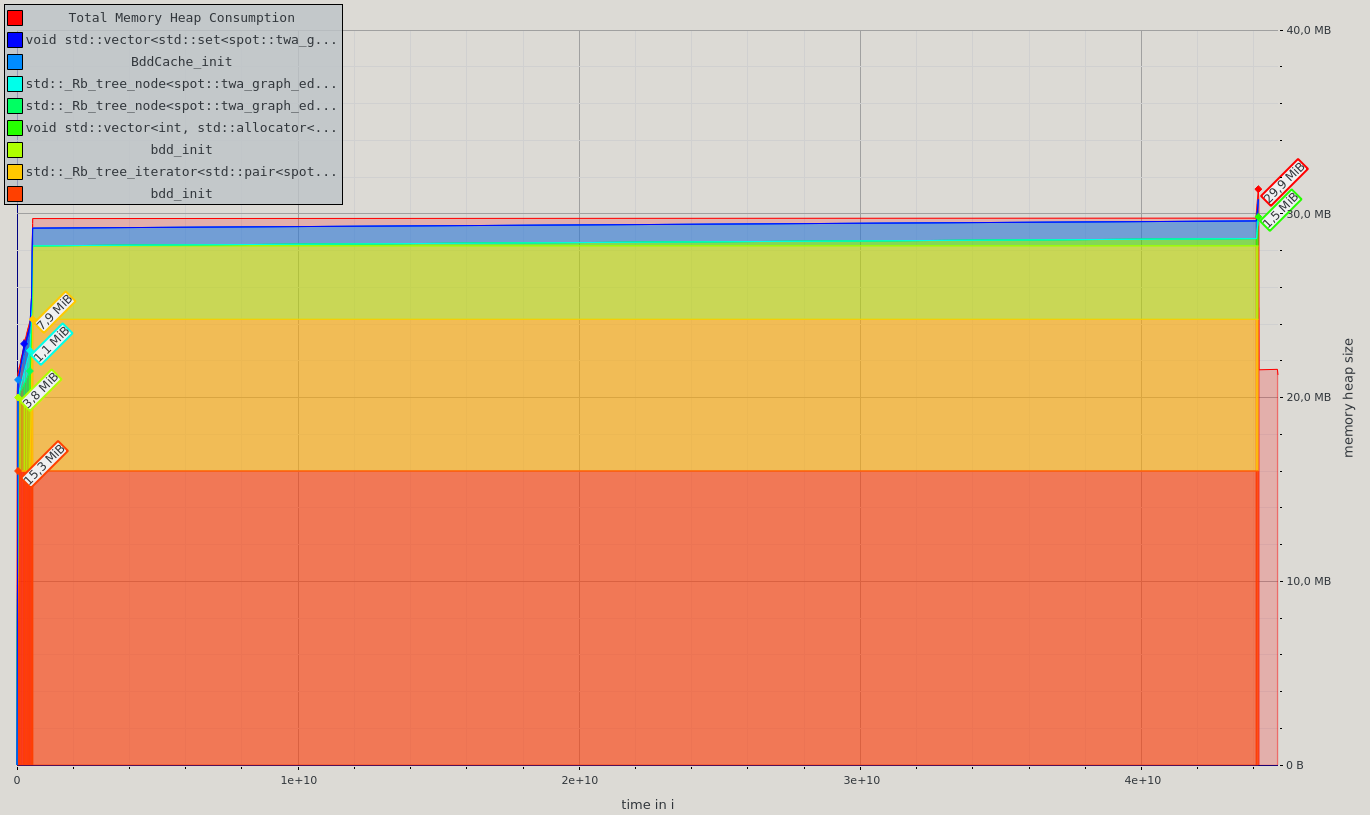
\includegraphics[scale=0.6]{img/memory_before.png}
 \caption{Memory heap consumption before optimizations}
 \label{fig:memory_before}
\end{figure}

\subsection{After Optimizations}
\begin{figure}[H]
 \centering
 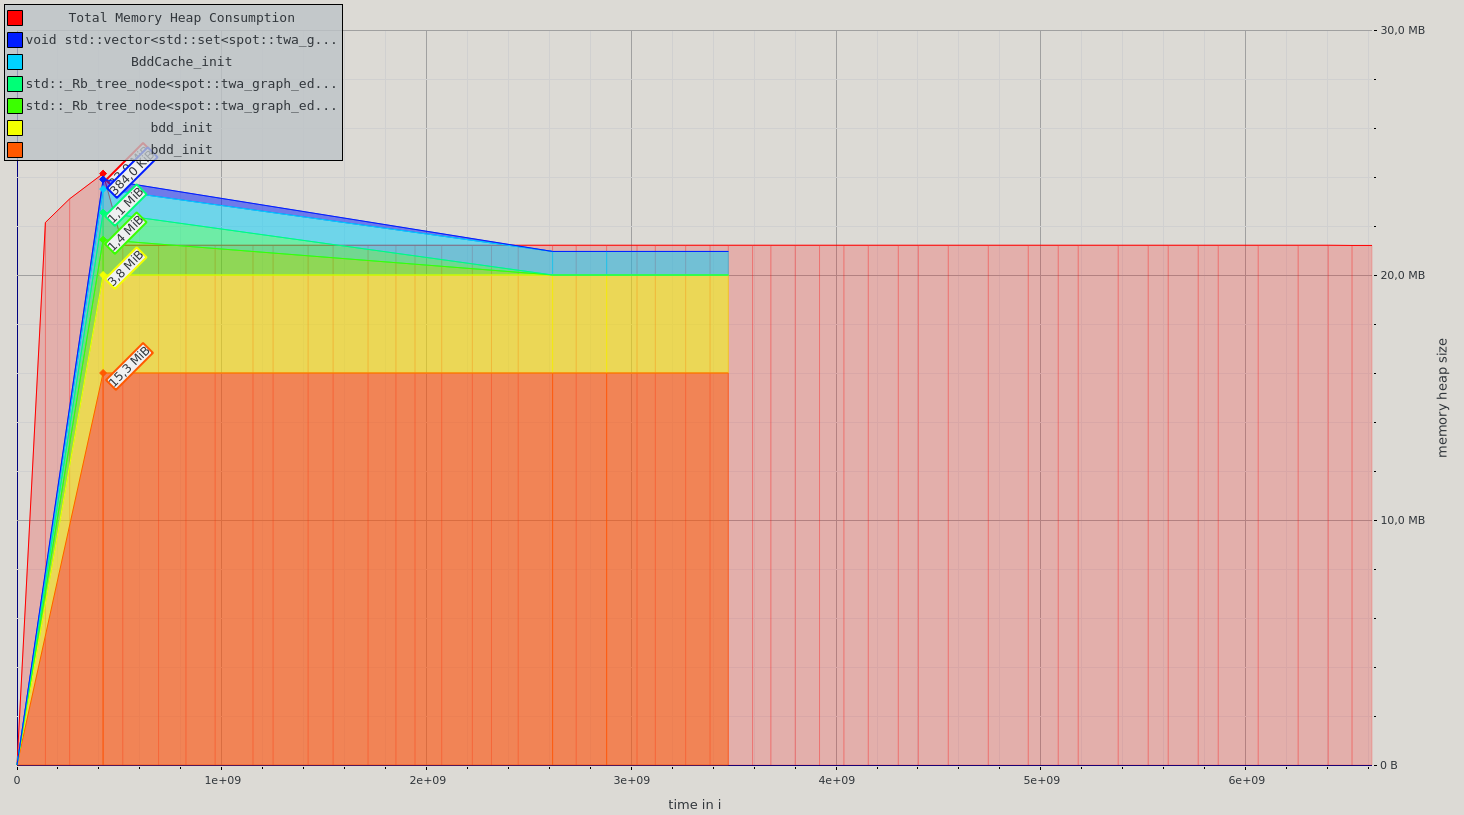
\includegraphics[scale=0.6]{img/memory_now.png}
 \caption{Memory heap consumption before optimizations}
 \label{fig:memory_now}
\end{figure}

\end{landscape}